\documentclass[11pt, oneside]{article}   	% use "amsart" instead of "article" for AMSLaTeX format
\usepackage{geometry}                		% See geom\dagetry.pdf to learn the layout options. There are lots.
\geometry{a4paper}                   		% ... or a4paper or a5paper or ... 
%\geometry{landscape}                		% Activate for for rotated page geometry
%\usepackage[parfill]{parskip}    		% Activate to begin paragraphs with an empty line rather than an indent
\usepackage{graphicx}				% Use pdf, png, jpg, or eps§ with pdflatex; use eps in DVI mode
\usepackage{array}							% TeX will automatically convert eps --> pdf in pdflatex		
\usepackage{amssymb}
\usepackage{cite}
\usepackage[final]{fixme}
\usepackage{pdfpages}
\usepackage{tabularx}
\usepackage{fancyheadings}
\usepackage{lastpage}
\usepackage{tikz}
\usetikzlibrary{shapes,arrows}
\usepackage{float}
\usepackage{hyperref}
\usepackage{url}

\parskip 6pt % 1pt = 0.351 mm
\parindent 0pt

%\title{Requirement Engineering Process in AMIDST}
%\author{The handsome AMIDST guys et. al.}
%\date{Latest version, \today}							% Activate to display a given date or no date

\pagestyle{fancy}
\lhead{\tiny FP7-ICT 619209 / AMIDST}
\chead{\tiny Page {\thepage} of \pageref{LastPage} \\}
\rhead{\tiny Public}
\renewcommand{\footrulewidth}{0.4pt}
\cfoot{}

\newcommand{\drop}[1]{}


\begin{document}

%\maketitle
%
%\begin{abstract}
%\end{abstract}
%



% Table of contents
\tableofcontents

\newpage

% Document History

\section*{Document history}

\begin{table}[htbp]
  \centering
  \begin{tabularx}{\linewidth}{|p{17mm}|p{17mm}|X|X|}\hline
    {\bf Version} & {\bf Date} & {\bf Author (Unit)} & {\bf Description} \\ \hline \hline
    v0.3 & 1/9 2014 &  & First draft finished  \\ \hline
\hline
  \end{tabularx}
\end{table}

\newpage


% Document History

\section{Executive summary}


 
\newpage

%\section{Introduction}

Even though the number of algorithms designed for learning on streaming data is increasing, there is still not a unified and well accepted way for evaluating them.  This is because testing and evaluating algorithms that are designed to work on streaming data are more difficult those designed to work on static data.  There are both statistical and computational reasons for this.  

Static data is data, where each instance can be assumed to be identically and independently distributed i.i.d.  On streaming data, one can often not assume that data instances are i.i.d.  Moreover, the algorithms are often designed to weight measurements that are close to the actual time step higher than measurements that are further back.  On streaming data, we must therefore assume that data are generated from underlying distributions that are time dependent and also that the algorithms themselves are time dependent.  

Computational challenges are related to the fact that the data come from an open-ended data stream, conceptually infinitely long, which imposes practical challenges related to restrictions on cpu-time and memory allocation.  

Various error measures related to stream data has been proposed in the papers of Gama et. al. \cite{Gam09}, \cite{Gam09_2}, \cite{Gam12}.  A loss function is typically related to the penalty of misclassifications on classification problems or residuals in regression models.  The holdout error is basically the average loss on a holdout dataset of fixed size.  The predictive sequential, or \emph{prequential} error is defined as the average loss function up to time step $i$, where $i$ is the current time step.  Moreover, it was also suggested to use a prequental error measure, which involved a forgetting factor such as using a time window or fading factors.  In paper \cite{Gam12}, convergence towards the Bayes error was shown for all these performance measures provided that the learners are consistent and data are i.i.d.  Moreover, it was shown that if data was allowed to drift over time, meaning that samples are only locally i.i.d, then the prequental error measures with forgetting mechanisms were favourable.

\todo{Relate to other work on streaming data as well.}

The applications that are covered in this report have different characteristics than the applications discussed in \cite{Gam12}.  Some problem will be evaluated on a holdout dataset assuming i.i.d and a stationary algorithm.  Other problems can not assume i.i.d on a local scale, but stationarity can be assumed on a larger time scale.  

In this paper we will establish formal procedures for testing and evaluating the developed models and algorithms. This includes specification what metrics are relevant to use to quantify the ability of the AMIDST system, such as relevant formalization of loss functions, maximum response-times, memory limits and output format.  The paper will also include 
considerations about what quantitative improvements AMIDST should obtain over state of the art.

In section \ref{sec:methodology}, AMIDST relevant methodologies for evaluation of both batch and streaming algorithms are identified and discussed.  This section forms the foundation of the subsequent sections, where the exact evaluation routines for each use case provider is given. These sections contains a description of the requirements related to evaluation as described in Delivery 1.2, a short description of the algorithms and the data and finally methods for evaluating predictive and runtime performances.  Section \ref{sec:conclusion} concludes the report.


%\quote{\emph{Task description: In this task we will establish formal procedures for testing and evaluating the
%    developed models and algorithms. This includes specification of maximum response-times, output format,
%    relevant formalization of loss functions, investigations into what metrics are relevant to use to quantify
%    the ability of the AMIDST system, and considerations about what quantitative improvements AMIDST should
%    obtain over state of the art.}}
%
%
%From Helge's slides at the WP 3 kickoff meeting:
%\begin{itemize}
%\item Massive datasets: find relevant techniques, ensure scalability, etc.
%\item Online evaluation of streams: find relevant techniques, ensure scalability, define behavior in changing environment, etc.
%\item Significance of results, e.g., considering changing environment vs. ``reproducability'', distribution for test-statistic, significance levels/sizes of test-sets, etc.
%\end{itemize}


\section{Preliminaries}\label{Section:Preliminaries}

%BN, OOBN, Dynamic BN.
%Preliminaries for the temporal series data analysis: correlograms, partial correlograms. %Preliminaries for the AMIDST models.

\section{Preliminary models}
\label{Section:PreliminaryModels}
\subsection{Daimler models}
\label{Section:DaimlerModels}


%\subsubsection{Introduction}

Daimler use-case is based on two application scenarios \cite{Fer14}: i) early recognition of a lane change manoeuvre; and ii) earlier prediction of the need for a lane change based on relative dynamics between two vehicles driving in the same lane at different speeds. 

The first scenario has been previously addressed by Daimler \cite{kasper2012object}. The main result of this previous work was a static object-oriented Bayesian network (OOBN) \cite{koller1997object} able to detect a manoeuvre 0.6 seconds before execution. The goal now is to enhance the prediction horizon for manoeuvre recognition by at least 1-2 seconds before execution to further improve the quality of the on-board adaptive cruise control. As we will explain later, this improvement is expected to be achieved by introducing a dynamic extension of the previously proposed static OOBN model. We basically consider such a dynamic extension for two main reasons: First, although with a limit prediction horizon, the static OOBN model has proven to be very robust for this task and it is considered as the gold-standard solution in Daimler. Second, the developed models in AMIDST project are expected to be integrated in an electronic control unit (ECU) \cite{Fer14}, so that the advances already made for the static model \cite{Weidl2014} could be exploited during the integration in the ECU of their dynamic counterparts. 

\subsubsection{Early recognition of a lane change manoeuvre}
\label{Section:Daimler:EarlyRecognition}

The basic settings of this application scenario are as follows: Let us suppose we are driving our car, referred to as EGO vehicle, in a highway. EGO vehicle is equipped with a video camera, radar, and some on-board sensors. Using the data provided by these sensors, the challenge consists in making an early recognition of a manoeuvre either by the EGO or any other relevant car in the traffic scene referred to as Object vehicle (OBJ). In total, the system is expected to recognise the following set of manoeuvres (a visual description of them is given below in Figure \ref{Figure:DaimlerManeuvers}):

\begin{enumerate}
\item \textbf{OBJ-CutIn}: A vehicle is moving to the lane where the EGO vehicle is placed.
\item \textbf{OBJ-CutOut}:  A vehicle that was driving in front of the EGO is leaving the EGO's lane.
\item \textbf{OBJ-Follow}: There is no lane change. The EGO is driving and there is another vehicle in front.
\item \textbf{LANE-Follow}: There is no lane change. The EGO is driving and there is no other vehicle in front.
\item \textbf{EGO-CutIn}: The EGO vehicle is moving right-direction to a new lane already occupied by another vehicle. 
\item \textbf{EGO-CutOut}: The EGO vehicle is leaving left-direction the lane where it was driving.
\end{enumerate}

\begin{figure}
\begin{center}
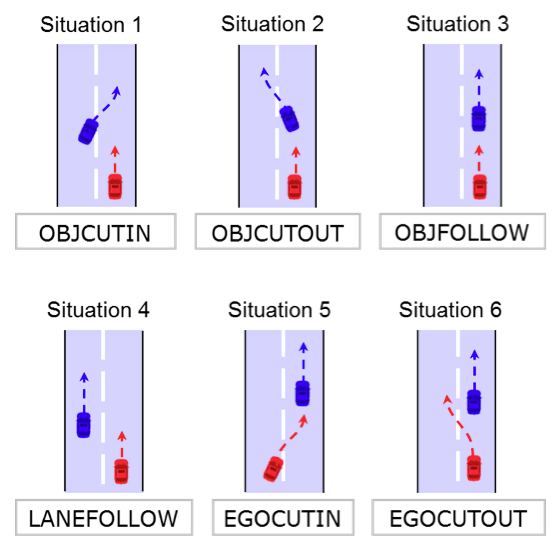
\includegraphics[scale=0.4]{./figures/DaimlerManeuvers}
\caption{\label{Figure:DaimlerManeuvers}The different manoeuvres to be identified by the AMIDST system. Red blocks represent the EGO vehicle while blue ones represent the Objet vehicle.}
\end{center}
\end{figure}

Instead of working directly with the raw data from the video, radar, and on-board sensors, the current manoeuvre recognition system uses the so-called ``object data'', which contains ``high level'' representations or features describing the traffic scene such as EGO's speed, distance between EGO and another vehicle in front, etc.  

\begin{figure}
\begin{center}
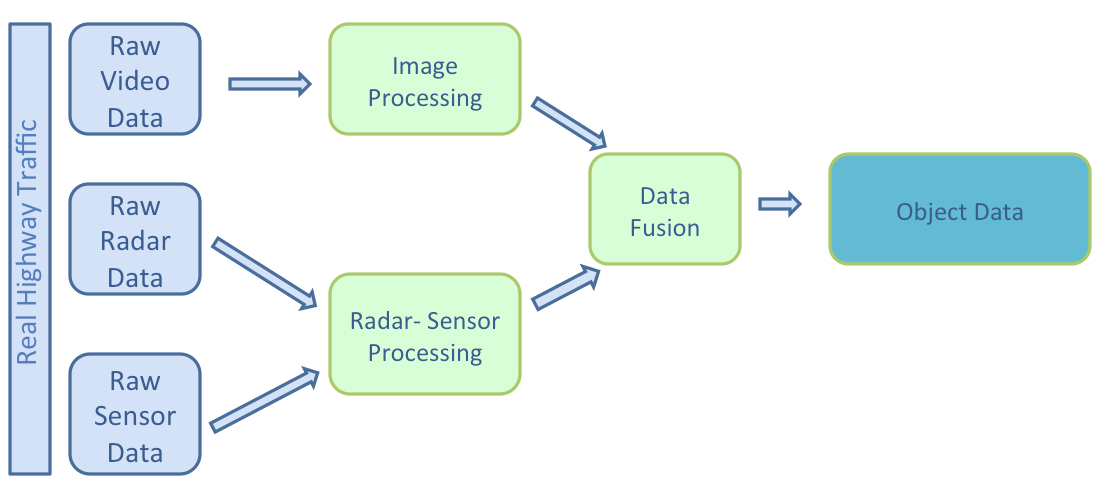
\includegraphics[scale=0.35]{./figures/DaimlerDataFlow}
\caption{\label{Figure:DaimlerDataFlow} Daimler's data flow.}
\end{center}
\end{figure}

Figure \ref{Figure:DaimlerDataFlow} contains a visual description of the current data flow used to create the ``object data''.  First, the raw data coming from the video, radar, and sensors are preprocessed. Then, the preprocessed data is merged, and the high-level or ``object data'' describing the traffic scene is obtained. 

As commented above, using the resulting ``object data'', Daimler has developed a probabilistic graphical model \cite{kasper2012object} which is able to recognize an ongoing manoeuvre around 0.6 seconds before it really takes place.  This probabilistic approach is based on modelling the problem in different abstraction layers. 


%The sensor data is modelled in the first layer. Using this layer, a new layer is created on top with the goal of detecting a lane change behaviour. The detection of a lane change behaviour allows the system to model the lane change manoeuvre in a higher layer. Finally, with this information, the system is able to identify the kind of driving manoeuvre which is taking place between a pair of vehicles. 
%
%
%
%\begin{figure}
%\begin{center}
%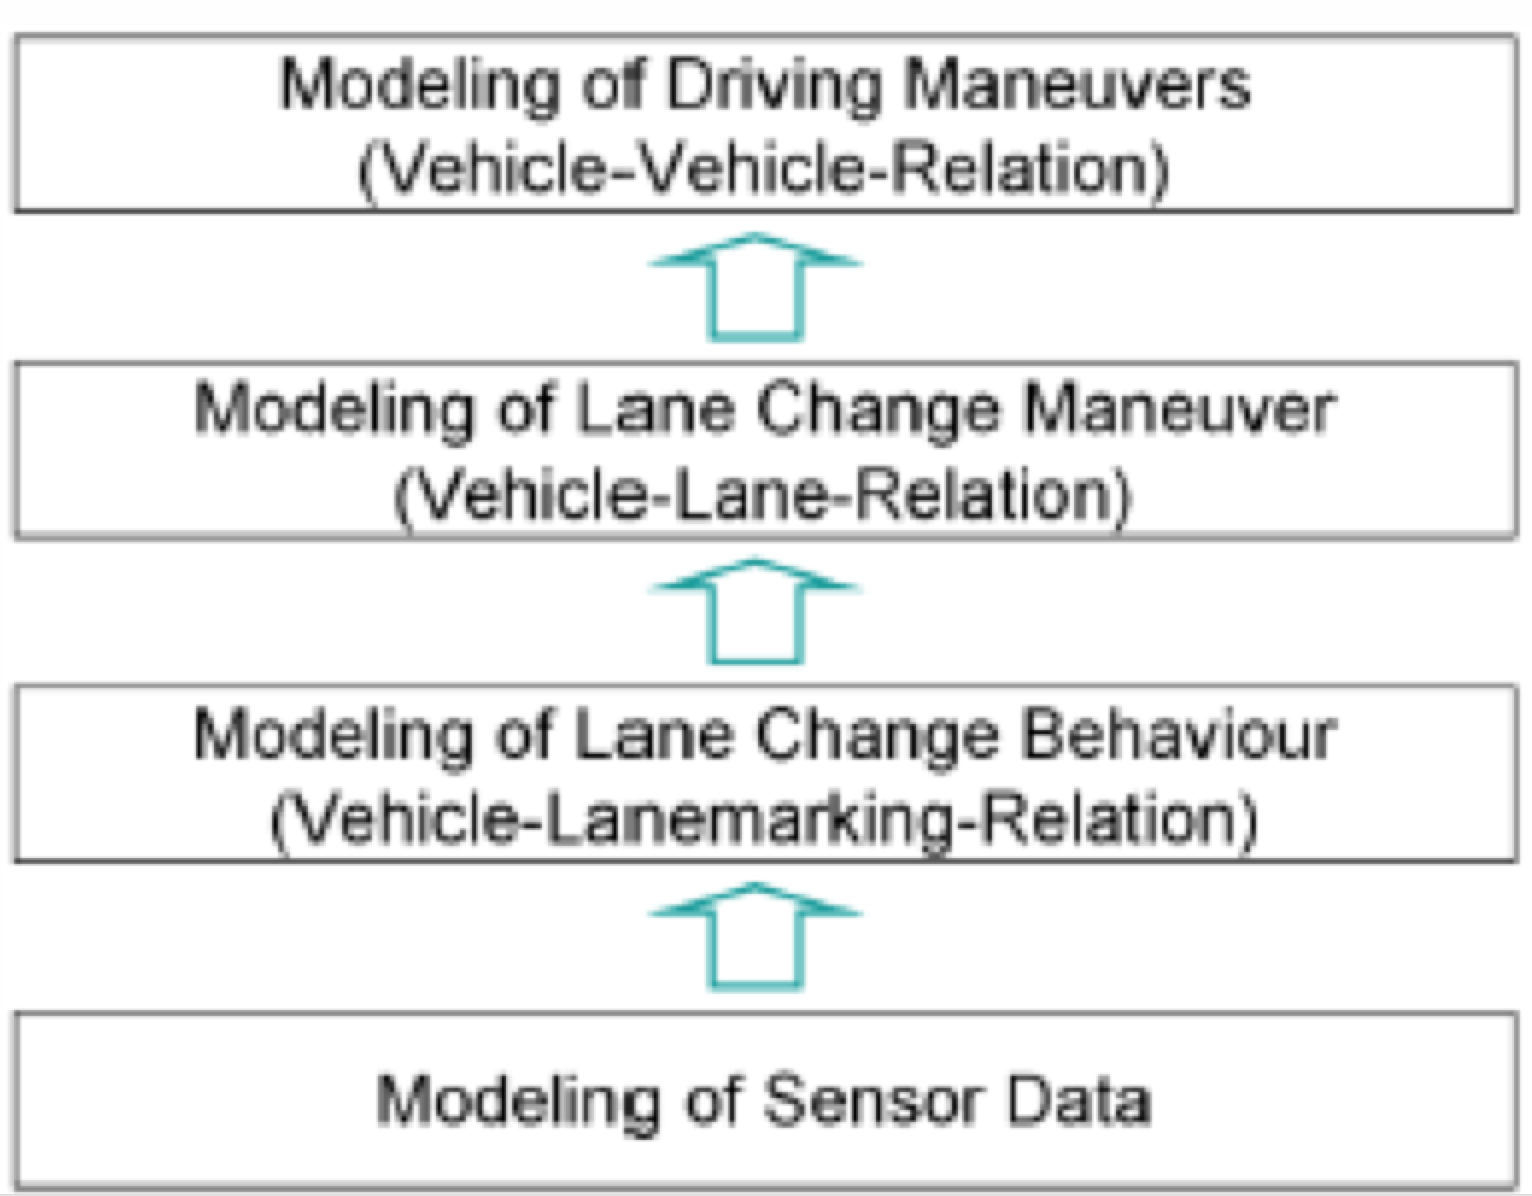
\includegraphics[scale=0.58]{./figures/DaimlerHierarchicalModelling}
%\caption{\label{Figure:DaimlerHierarchicalModelling} Hierarchical layers for the recognition of driving manoeuvres.}
%\end{center}
%\end{figure}

\subsubsection*{Static OOBN model}

The model described here was presented in \cite{kasper2012object} as an object-oriented Bayesian network (OOBN) \cite{koller1997object} for addressing the problem of early recognition of a lane change manoeuvre (application scenario 1).  This model works with the so-called ``object data''. This data mainly consists of a set of measured and/or computed signals or situation-features denoted by $S$ (e.g. EGO speed, EGO lateral velocity, speed of a car in-front, etc., see \cite{kasper2012object} for further details) describing the traffic scene. The situation features used for manoeuvre recognition are structured along three main dimensions: lateral evidence (LE), trajectory (TRAJ), and occupancy schedule grid (OCCGRID).  A visual description is given in Figure \ref{Figure:DaimlerSituationFeatures}. They are referred to as the three possible hypotheses of a lane change manoeuvre: 1) LE hypothesis considers the lateral offset and the lateral velocity of a car and accounts for its lateral movement; 2) TRAJ hypothesis accounts for the evidence about a car's trajectory by using the measures of the car angle and the estimated time to crossing the line; and 3) OCCGRID hypothesis allows to identify if a car surroundings are going to be occupied by some other vehicle in the traffic scene. 

\begin{figure}
\begin{center}
\begin{tabular}{ccc}
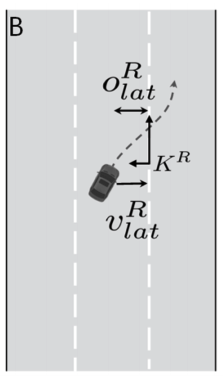
\includegraphics[scale=0.5]{./figures/DaimlerLEHipothesis} &

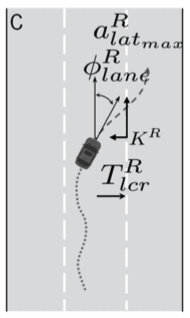
\includegraphics[scale=0.5]{./figures/DaimlerTRAJHipothesis} &

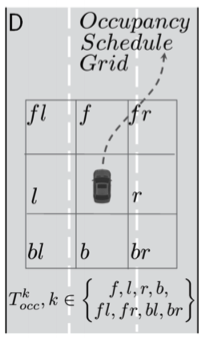
\includegraphics[scale=0.5]{./figures/DaimlerOCCGRIDHipothesis} \\

Lateral evidence & Trajectory & Occupancy grid \\
\end{tabular}
\caption{\label{Figure:DaimlerSituationFeatures} The three main dimensions of the situation features \cite{kasper2012object}.}
\end{center}
\end{figure}

%The whole modelling is structured in hierarchical layers as detailed in Figure \ref{Figure:DaimlerHierarchicalModelling} and it has been previously implemented \cite{kasper2012object} using an object-%oriented Bayesian network (OOBN) \cite{koller1997object}. 
%Even using this high-level features, the modelling problem is very complex. 
%At the same time, the problem contain a lot of structure and can be divided in simpler and similar sub-problems. For example, when deciding whether there is evidence or not that a car is performing a %lateral movement to the right, we can employ two situation-features such as the lateral velocity to the right and the lateral offset w.r.t. the right lane marking of this vehicle to make this decision. But %we will find a quite similar problem when deciding about the lateral movement evidence of the EGO car or any other car, when the only difference that will use another situation-features (e.g. the right %lateral velocity of the EGO) .

The general structure of this OOBN model consists of a number of abstraction levels as detailed in Figure \ref{Figure:DaimlerOOBNAbstraction}: 

\begin{description}
\item[Class sensor measurement:]  This class represents objects at the lowest level of the OOBN. It models the so-called \textit{measured data} which are  the observations characterising a situation. They are acquired from sensors and computations (see Figure \ref{Figure:DaimlerDataFlow}). The structure is the common one found in a standard Kalman filter model to account for sensor noise or fault: S\_MEAS refers to the sensor-reading value, S\_REAL refers to the real value, and S\_SIGMA refers to the uncertainty in the measurements. In this way, the sensor-reading of a measured variable (S\_MEAS) is conditionally dependent on random changes in the real value under measurement (S\_REAL) and sensor noise/fault (S\_SIGMA). In Daimler, the observations of the measured value S\_MEAS and the uncertainty of the measurement S\_SIGMA are given in the object data. 

\item[Class hypothesis:] This class pertains to a higher level and directly depends on the real values S\_REAL obtained in the previous class. In fact, the real sensor values are used to evaluate the different possible hypotheses namely LE, TRAJ and OCCGRID. 

\item[Class event:] This class is at the top level of the modelling. It allows to model high-level Hypothesis/Event based on low-level hypotheses ($Hypothesis_1, \ldots, Hypothesis_n$) in a recursive way. This class also includes the event variable representing the possible traffic manoeuvres of the own and neighbour vehicles. 
\end{description}

\begin{figure}
\begin{center}
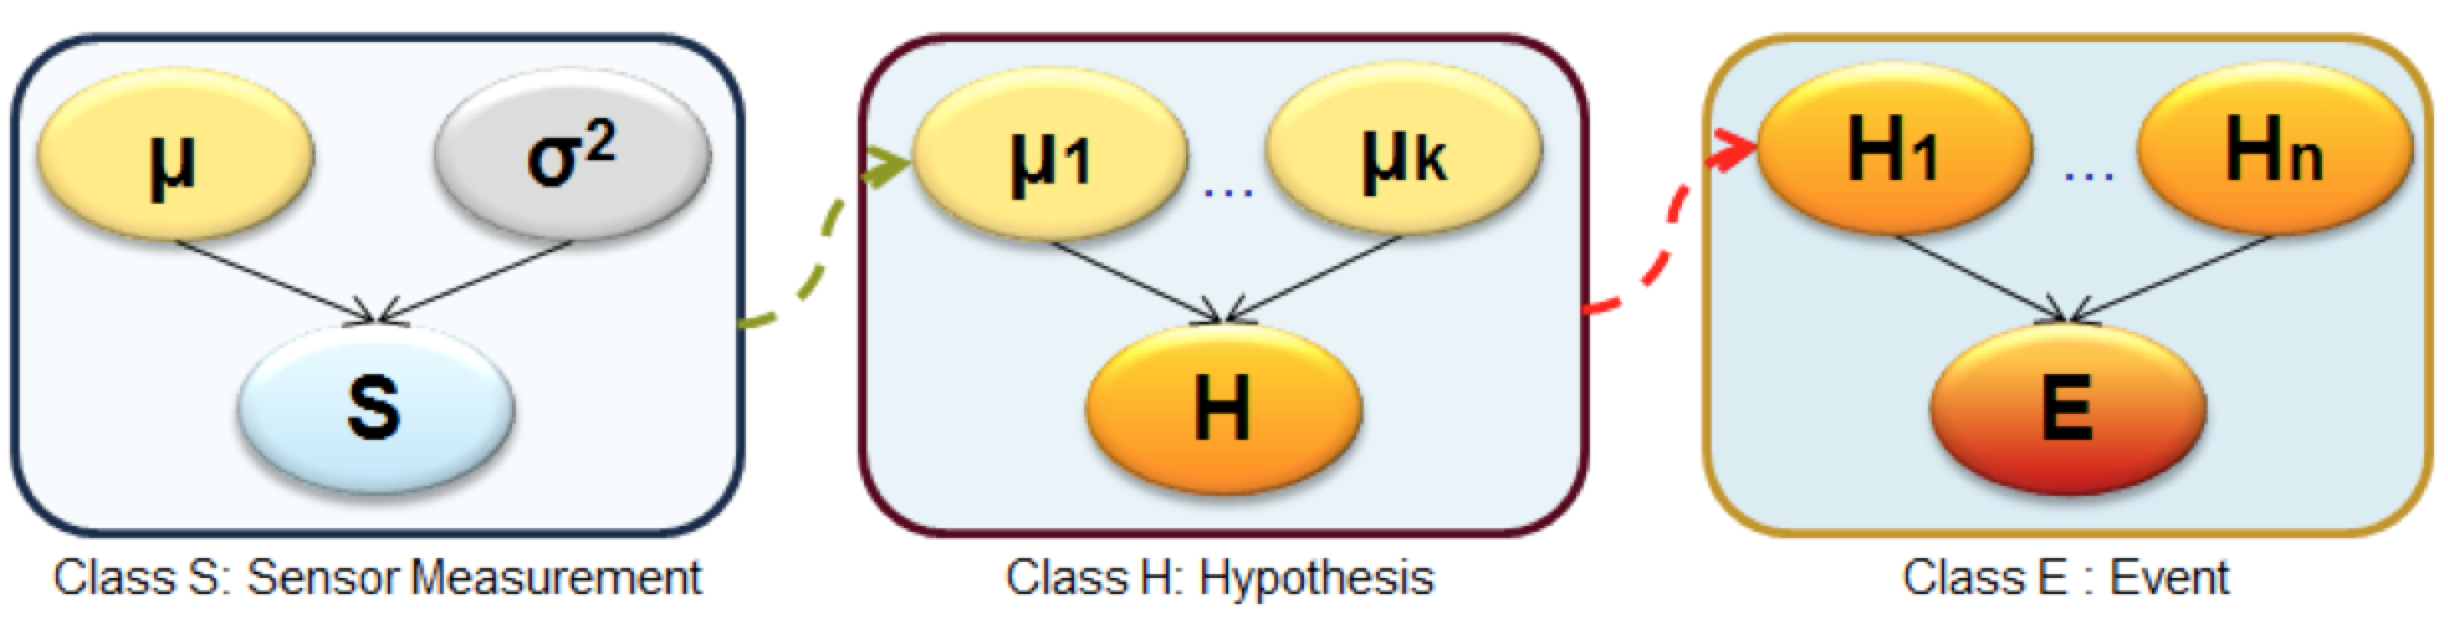
\includegraphics[scale=0.58]{./figures/DaimlerOOBNAbstraction}
\caption{\label{Figure:DaimlerOOBNAbstraction} Static-OOBN model for the prediction of an event (manoeuvre) \cite{Weidl2014}.}
\end{center}
\end{figure}

Finally, Figure \ref{Figure:DaimlerLE} shows a concrete fragment of the static OOBN model related to the LE hypothesis modelling. As it can be seen, LE hypothesis depends on the lateral offset to a lane marking, O\_LAT\_REAL, as well as on the lateral velocity, V\_LAT\_REAL, of the car. Both measures are estimated from their measured values, O\_LAT\_MEAS and V\_LAT\_MEAS, respectively, and from the estimated uncertainty of the measurements,O\_LAT\_SIGMA and V\_LAT\_SIGMA. This OOBN fragment is used to model the growing probability for LE to cross the lane marking, based on the vehicle coming closer to the lane marking and the increase of its lateral velocity.

\begin{figure}
\begin{center}
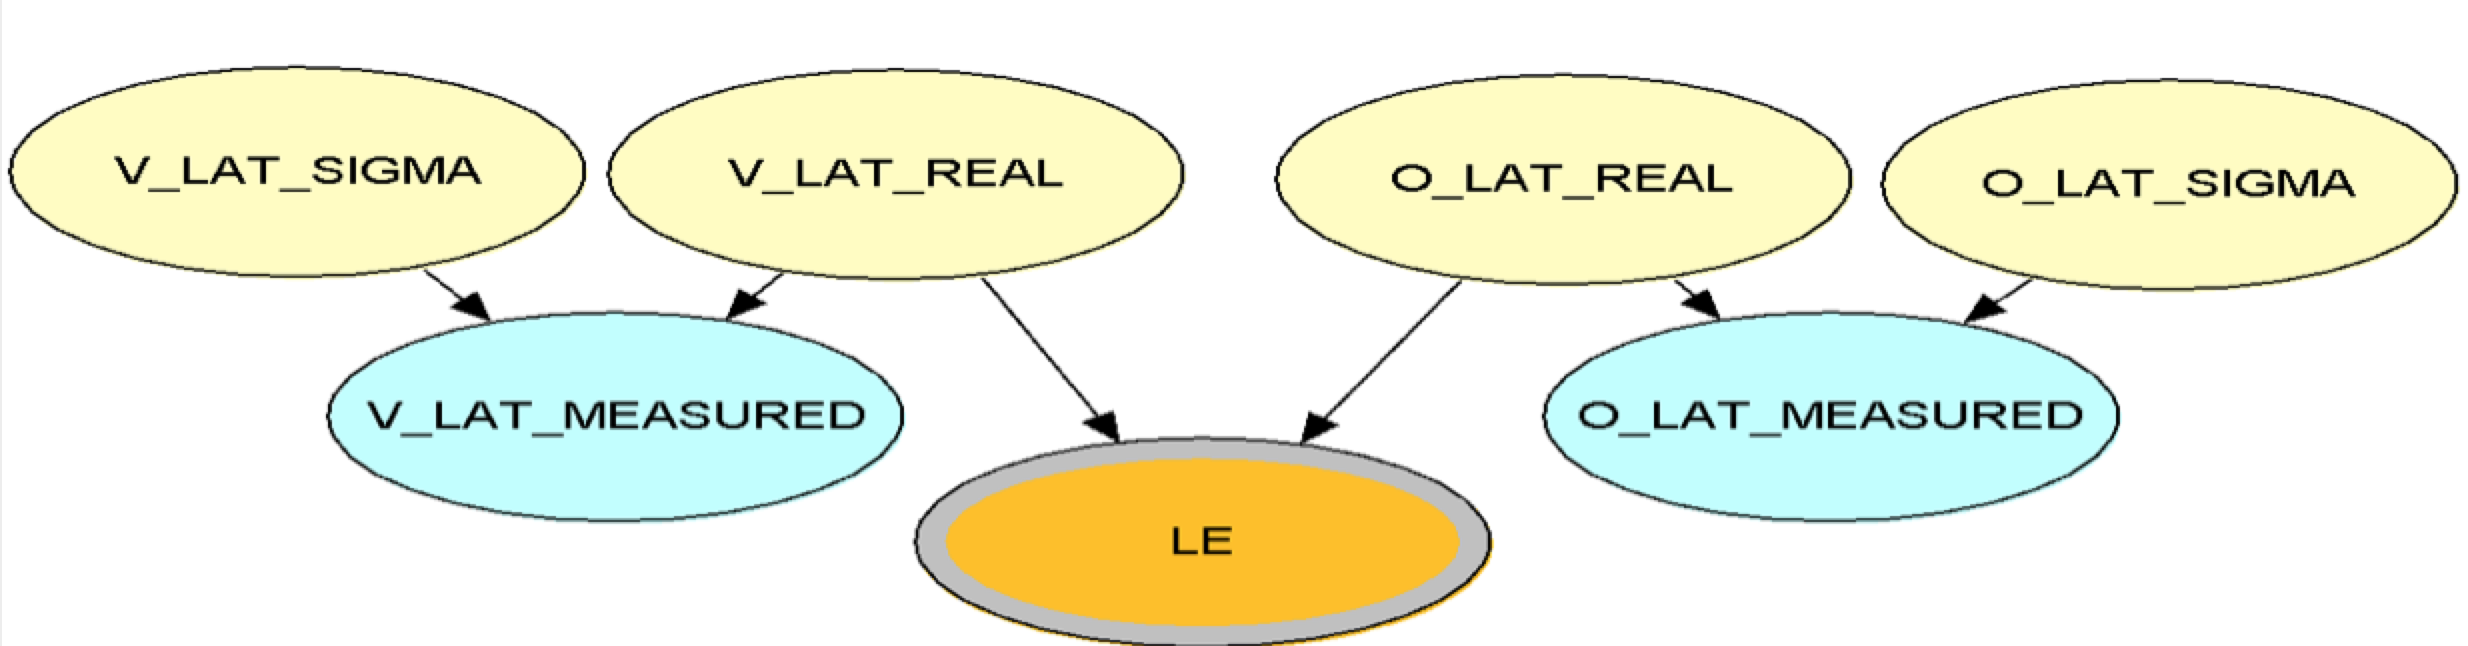
\includegraphics[scale=0.58]{./figures/DaimlerLE}
\caption{\label{Figure:DaimlerLE} Static OOBN fragment for the lateral evidence hypothesis.}
\end{center}
\end{figure}


These models contain both continuous and discrete variables. They were parametrized using the CLG framework \cite{JensenNielsen2007,lauritzen1996graphical} for continuous children with continuous parents and multinomial distributions for discrete children with discrete parents. In these models we also have the case of discrete children with continuous parents (i.e. low-level hypothesis depending of S\_REAL variables) that were initially parametrized by a logistic function. However, as discussed in Section \ref{Section:Preliminaries}, this modelling has significant impact when making inference. A possible solution used in \cite{kasper2012object} is to discretize S\_REAL variables. In this case, because S\_MEAS, S\_SIGMA are always observed their potentials can be collapsed/combined with the potential of the respective discretized S\_REAL variables. And, therefore, all the inferences in this probabilistic model can be made by only using discrete potentials \cite{nielsen2009bayesian}.


\subsubsection*{The dynamic-OOBN model}\label{Section:DaimlerDynamic}

The above described static OOBN is able to detect a manoeuvre $0.6$ seconds before execution. As detailed in the DoW \cite{Fer14}, the goal is to enhance the prediction of manoeuvre recognition to at least $1-2$ seconds (max.\ $4-5$ seconds) before the actual lane marking crossing. Moreover, this early detection of the manoeuvre should not be at the expense of the prediction accuracy. As specified in Daimler's DoW \cite{Fer14}, the area under the ROC curve (AUC) should be greater than 0.96 for 1 second and greater than 0.9 for 2 seconds.

Figure \ref{Figure:daimlerTPlot} shows an example of the performance and limitations of the current static-OOBN model. Two randomly selected sequences, namely seq1 and seq2, where the behaviour of two cars, EGO and OBJ is considered. 

\begin{figure}[ht!]
\begin{center}
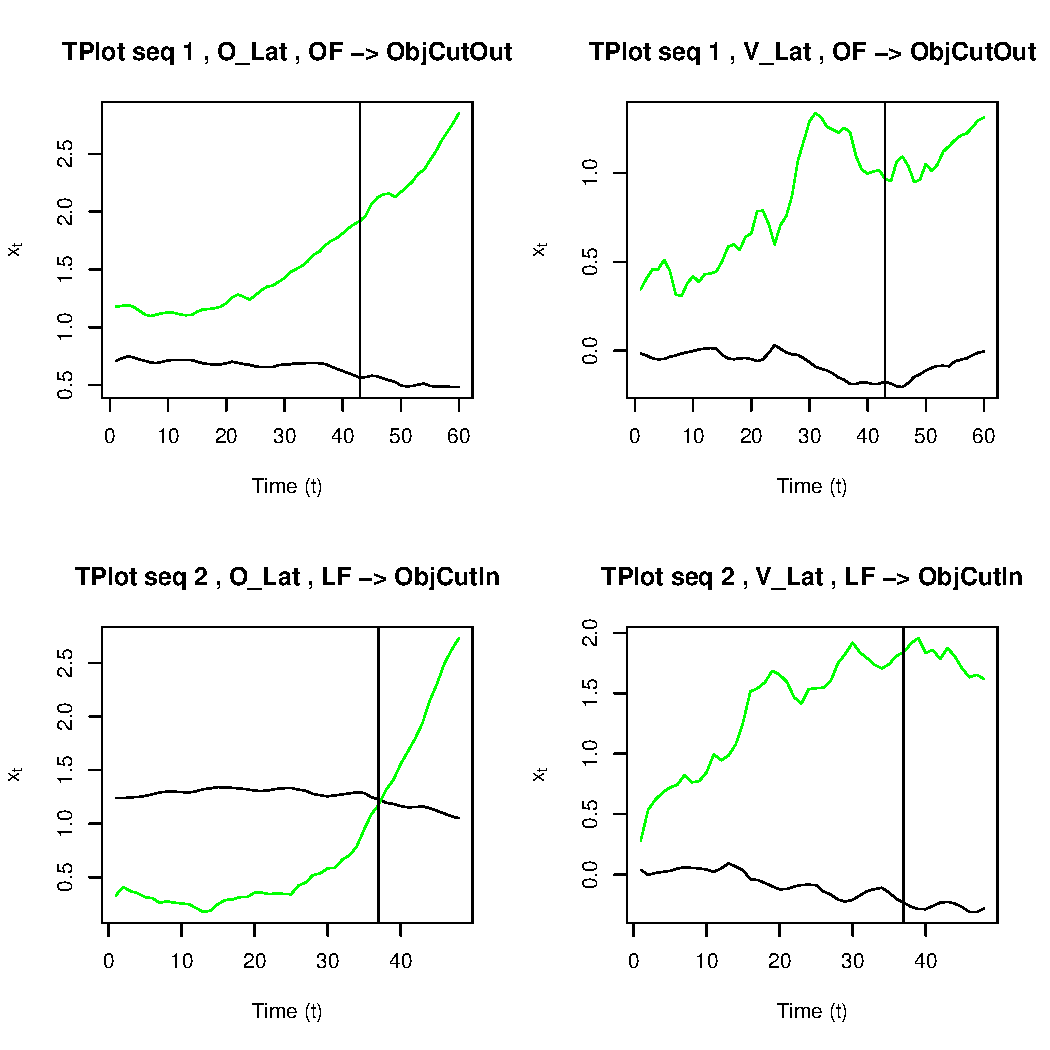
\includegraphics[scale=0.65]{./figures/DaimlerLE_EGO_L_LE_OBJ_R_OBJCut.pdf}
\caption{\label{Figure:daimlerTPlot}Time plots of the lateral velocity (V\_Lat) and the lateral offset (O\_Lat) for EGO (black curves) and OBJ (green curves) in two randomly selected sequences of an ObjCutOut (seq 1) and an ObjCutIn (seq 2). The x-axis corresponds to the different time-steps and the y-axis to the lateral offset on the left-hand side graphs and lateral velocity on the right-hand side graphs.}
\end{center}
\end{figure}

In these figures, we plot the evolution of different time-steps for lateral offset (O\_Lat) and lateral velocity (V\_Lat) to a lane marking in ongoing OBJ-CutOut and OBJ-CutIn manoeuvres. In each figure, the vertical black bar indicates the moment in which the manoeuvre has been recognised by the current static OOBN model. The manoeuvre is finished at the end of the series, which coincides with the actual moment of changed lane. The black curve corresponds to the lateral offset and lateral velocity of the EGO car, which is just following the lane (LF), while the green curve corresponds to the values of the OBJ car performing the OBJ-CutOut/OBJ-CutIn manoeuvres. As expected for lane follow (LF), the lateral velocity of the EGO fluctuates around zero (i.e., EGO car is just driving inside its lane) and the lateral offset of the lane marking is almost constant all the time. However, when we look at the lane change behaviour of the OBJ car (green curves), we easily see a different behaviour. Firstly, we observe that the lateral velocity is much  higher, indicating a lateral movement. Similarly, we also observe how the lateral offset steadily increases, what clearly indicates that the OBJ car is leaving its current lane in both manoeuvres. 


Although the manoeuvre is clearly identified before it completes in both considered sequences, it is desired to predict it \textit{further} in advance. Looking at the evolution of lateral offset and velocity in Figure \ref{Figure:daimlerTPlot}, we could argue that the detection of the manoeuvre can be performed earlier (i.e., when the lateral offset and lateral velocity starts to increase more dramatically and consistently for \textit{several} time-steps). This is one of the basic pieces of evidence that motivates the development of the dynamic version of the static-OOBN model \cite{Weidl2014}. 


\begin{figure}[ht!]
  \centering
    \begin{tabular}{cc}
    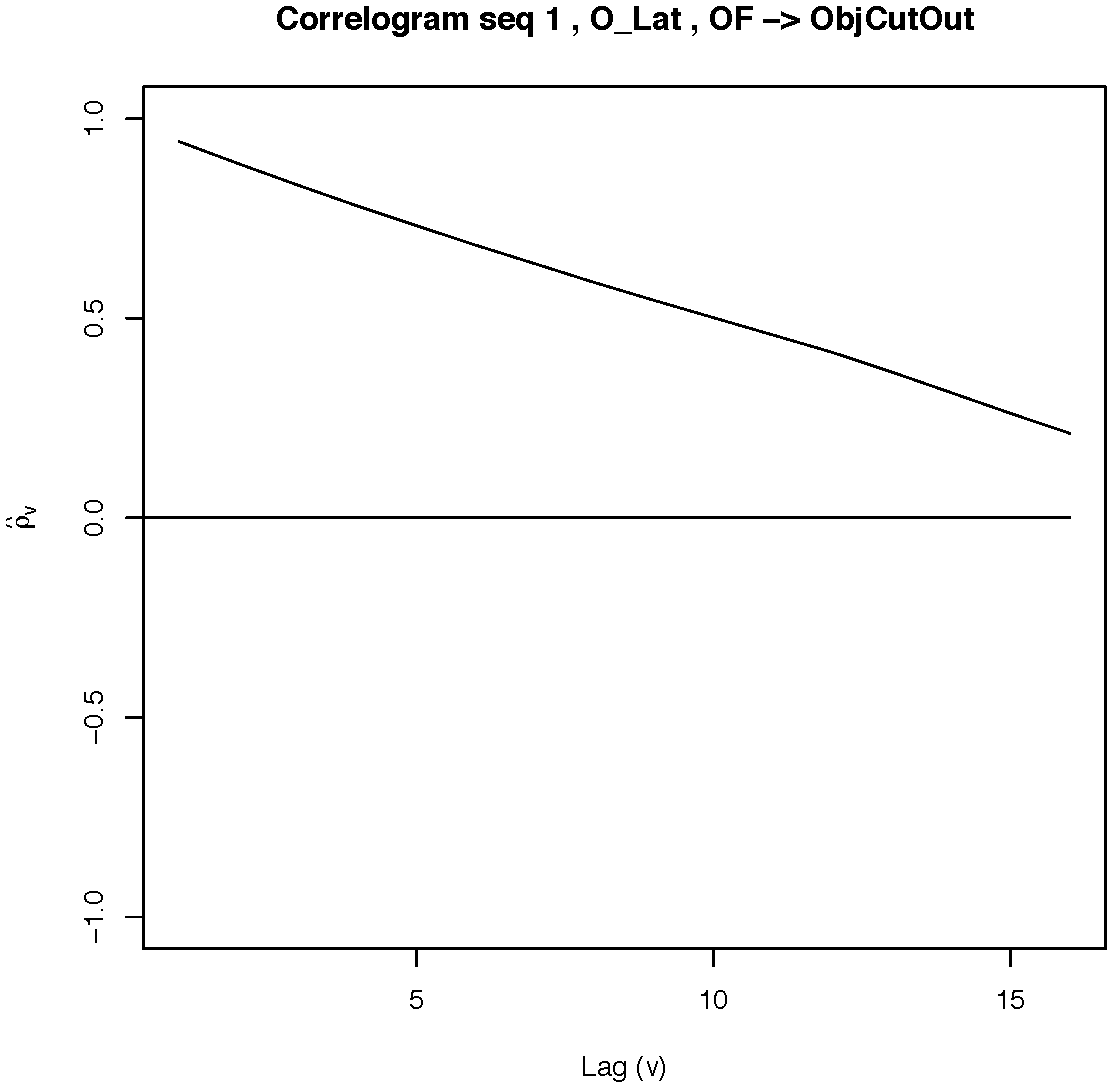
\includegraphics[width=60mm]{figures/DaimlerCorrOBJ_R15Offs.pdf}&
    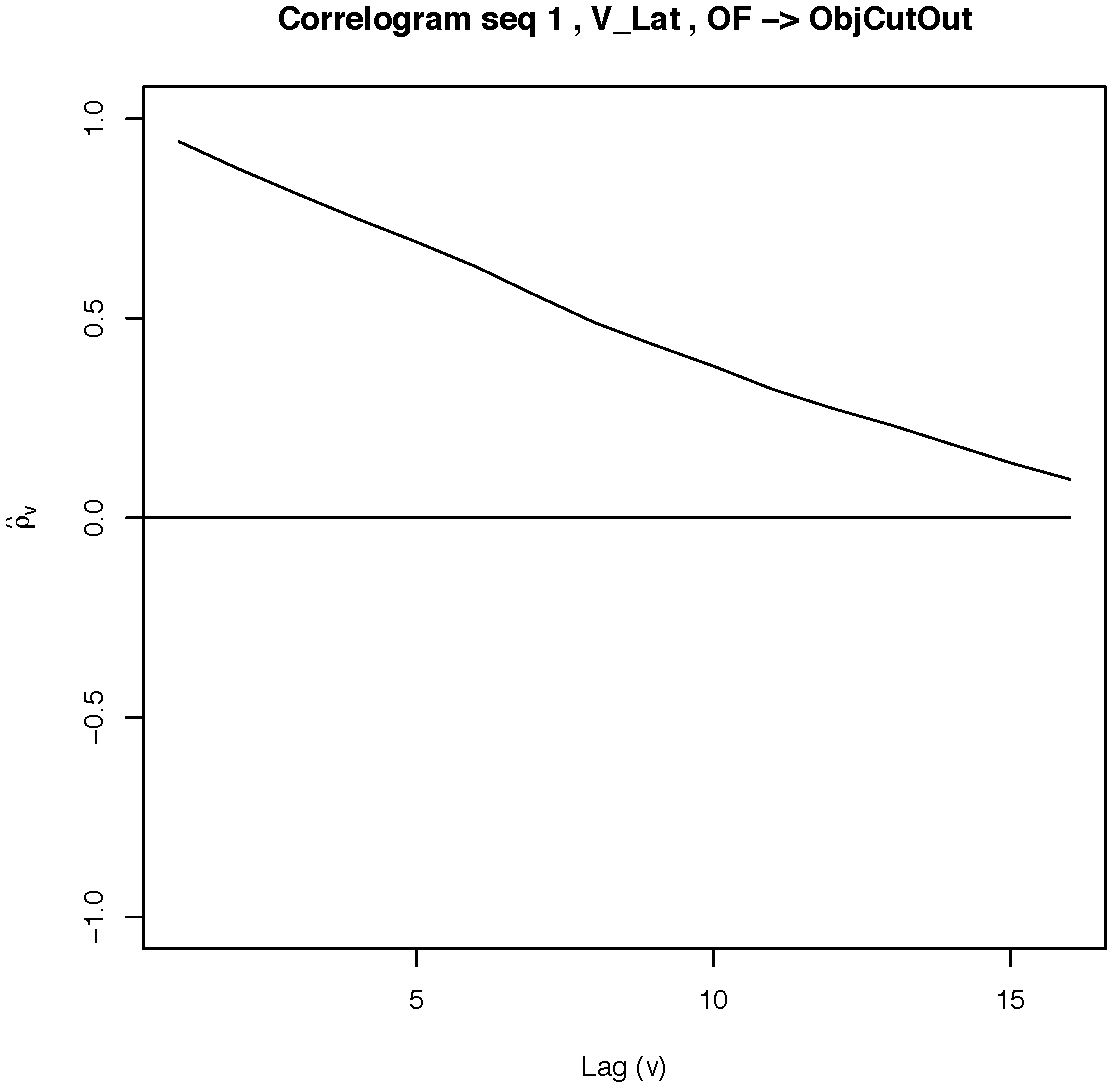
\includegraphics[width=60mm]{figures/DaimlerCorrOBJ_R15Vel.pdf}\\
  \end{tabular}
    \caption{\label{Figure:daimlerCorrel}Correlograms for lateral velocity and offset. The x-axis represents the lag $v$ or time difference, and the y-axis represents the sample autocorrelation coefficient of lag $v$, denoted by $\hat{\rho_v}$, i.e., the correlation between variables at times $t$ and $t+v$ (see Section \ref{Section:Preliminaries} for more details).}
\end{figure}

In any case, let us note, that the prediction horizon for manoeuvre recognition is going to be limited in order to avoid false positives (i.e. recognizing a lane change manoeuvre when the driver was just performing some random lateral movement).  In case of a false positive, such as an erroneously OBJ-CutIn for instance, the adaptive cruise control would react with an unnecessary break, so they ought to be avoided. It is then required to find a good balance between the rate of false positives and false negatives. 

An additional piece of evidence that motivates the use of dynamic models appears when we look at the sample correlograms for lateral velocity and offset (that is, the correlation of the data with lagged values of themselves) plotted in Figure \ref{Figure:daimlerCorrel}. There we can see a strong temporal dependency (the correlation coefficients are high) for the two variables when we consider a \textit{small} number of time-steps between the temporal observations. Hence, the use of a dynamic model to make predictions about the evolution of the lateral velocity and lateral offset in a near future seems to be reasonable according to this analysis. Moreover, our main assumption is that the use of dynamic Bayesian network models (see Section \ref{Section:Preliminaries}) will allow us to build a more accurate and reliable system for manoeuvre recognition. 

As explained in Section \ref{Section:Preliminaries}, the dynamic extension involves copies of the static OOBN for different number of time steps in the time window. Figure \ref{Figure:daimlerLEdyn} shows an example for the LE hypothesis, where the nodes for O\_LAT\_REAL and V\_LAT\_REAL are temporal clones defining the belief state between consecutive time steps, and hence creating a first order Markov process. This model has been proposed in \cite{Weidl2014} by some of the AMIDST partners. The first order assumption is a standard assumption in this kind of models and helps to simplify the posterior inference and learning process. Fortunately, if we build a partial correlogram as the ones plotted in Figure \ref{Figure:daimlerPartialCorrel}, we can see that this assumption seems reasonable, because the influence of the lateral offset at time $t-1$ on the lateral offset at time $t+1$ given the lateral offset at time $t$ is close to null (i.e., the value at $v=2$ for the lag is close to null in Figure \ref{Figure:daimlerPartialCorrel}). Note that the same reasoning applies also to the lateral velocity.

\begin{figure}[ht!]
\begin{center}
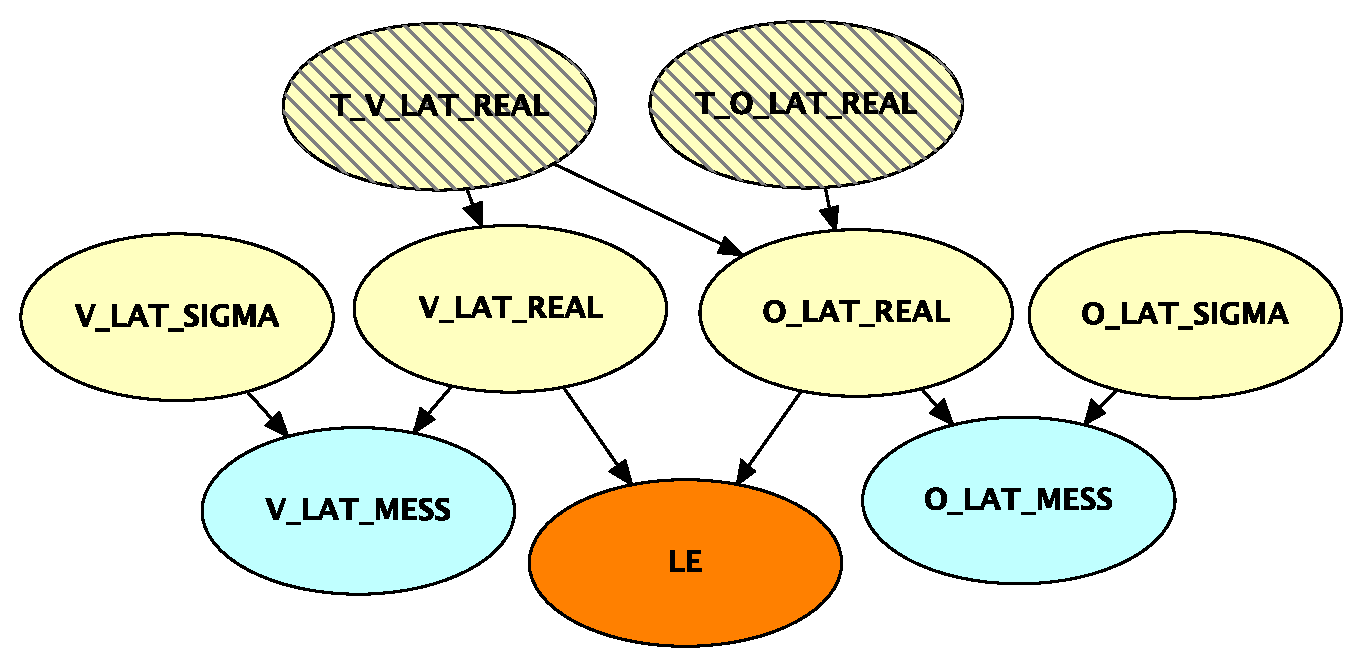
\includegraphics[scale=0.48]{./figures/DaimlerLEdyn}
\end{center}
\caption{\label{Figure:daimlerLEdyn}Daimler dynamic OOBN fragment for LE hypothesis.}
\end{figure}

\begin{figure}[ht!]
  \centering
    \begin{tabular}{cc}
        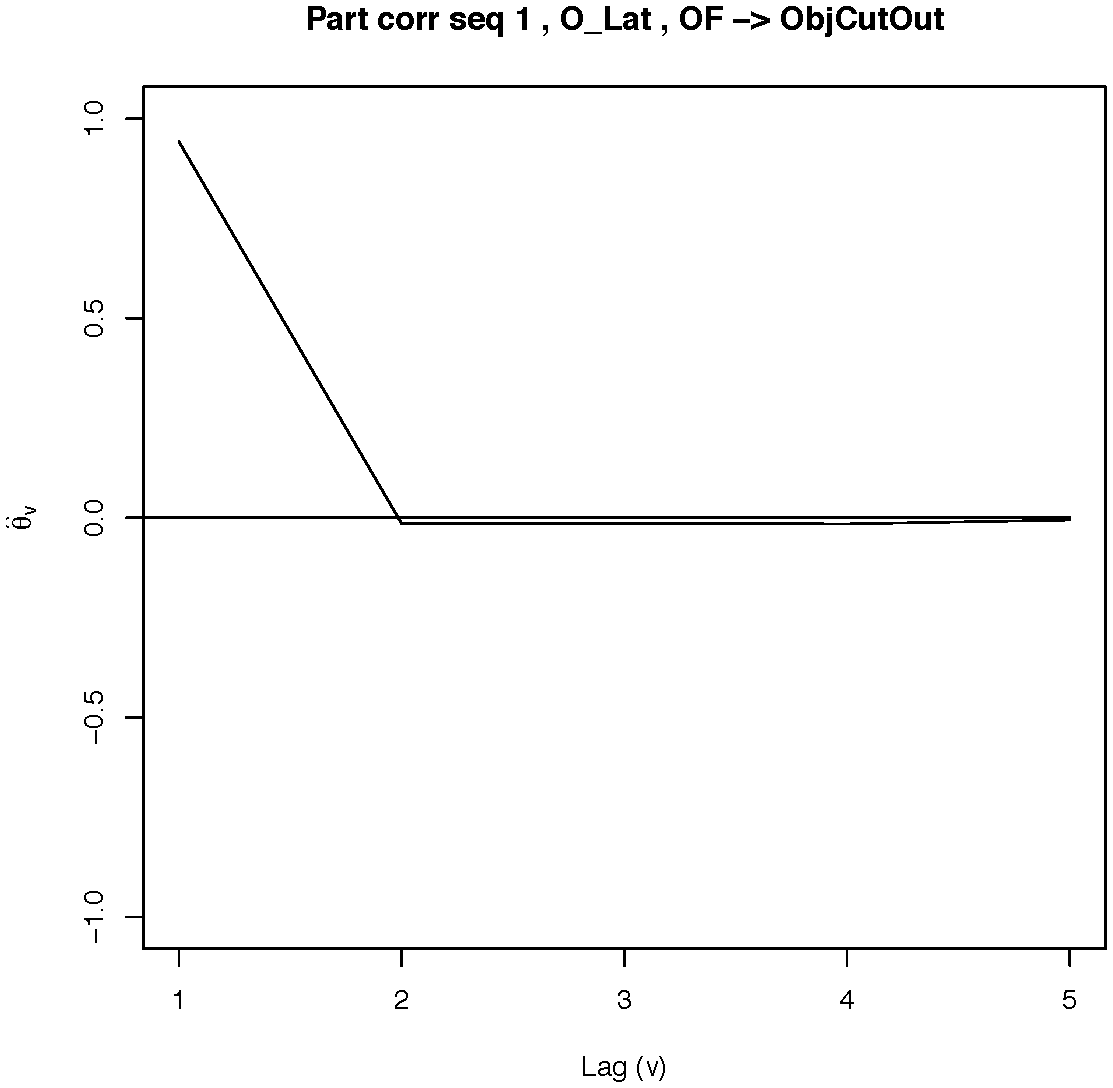
\includegraphics[width=60mm]{figures/DaimlerPcorrOBJ_R5Offs.pdf}&
    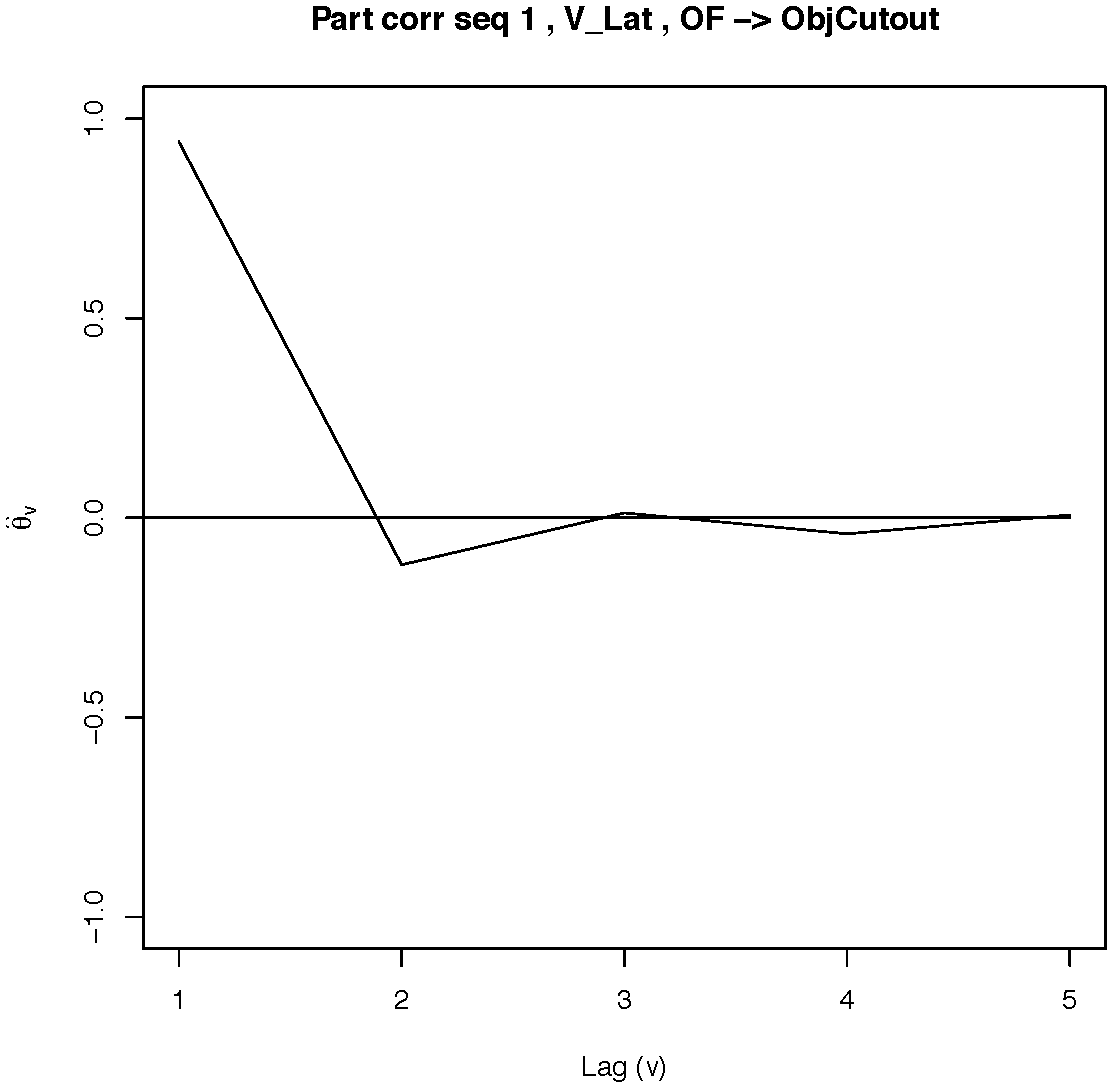
\includegraphics[width=60mm]{figures/DaimlerPcorrOBJ_R5Vel.pdf}\\
  \end{tabular}
    \caption{\label{Figure:daimlerPartialCorrel}Partial correlograms for lateral velocity and offset. The x-axis represents the lag $v$ or time difference, and the y-axis represents the partial autocorrelation coefficient of lag $v$, denoted by $\ddot{\theta_v}$, i.e., the correlation between variables at times $t$ and $t+v$ after having removed the common linear effect of the data in between (see Section \ref{Section:Preliminaries} for more details).}
\end{figure}

As described in \cite{Weidl2014}, the proposed DBN aims to incorporate the trend of change for the real values, where their physical relations are represented as causal dependencies between the time-steps $dt$. For instance, in Figure \ref{Figure:daimlerLEdyn}, the transition function of O\_LAT\_REAL at time $t$, denoted as $O(t)$, is modelled as a Gaussian distribution. Its mean is affected by $O(t-1)$, and by V\_LAT\_REAL at time $t-1$, denoted as $V(t-1)$. Therefore, we have:

\begin{equation}
O(t) =O(t-1) +V(t-1)dt +\epsilon
\end{equation}

where $\epsilon$ denotes a white noise $\mathcal{N}(0,\sigma^2)$ which is assumed to be small. In order to corroborate the validity of this distributional assumption, we also analysed the hypothesis $O(t) - O(t-1) = \Delta O = V(t-1)dt +\epsilon$ on our data. Figure \ref{Figure:daimlerVvsOffs} shows the time and bivariate contour plots for $V(t-1)$ and $\Delta O$ for a randomly selected sequence (i.e., Seq 7) of an OBJ-CutOut manoeuvre. Both plots clearly prove that the assumption of a linear relationship with Gaussian noise might not be very far from reality.

The avid reader may have also noticed that these approaches do not take acceleration into account, i.e., they assume that it is constant at all times. From time plots corresponding to velocity in Figure \ref{Figure:daimlerTPlot}, we can easily observe that this is an unrealistic assumption. A more detailed analysis about the possible future inclusion of acceleration in the dynamic models is included below in Section \ref{subsubsection:daimlerfuture}, where future models are discussed.

\begin{figure}[ht!]
  \centering
  \setlength{\tabcolsep}{0.05pt}
  \renewcommand{\arraystretch}{0.02}
    \begin{tabular}{cc}
    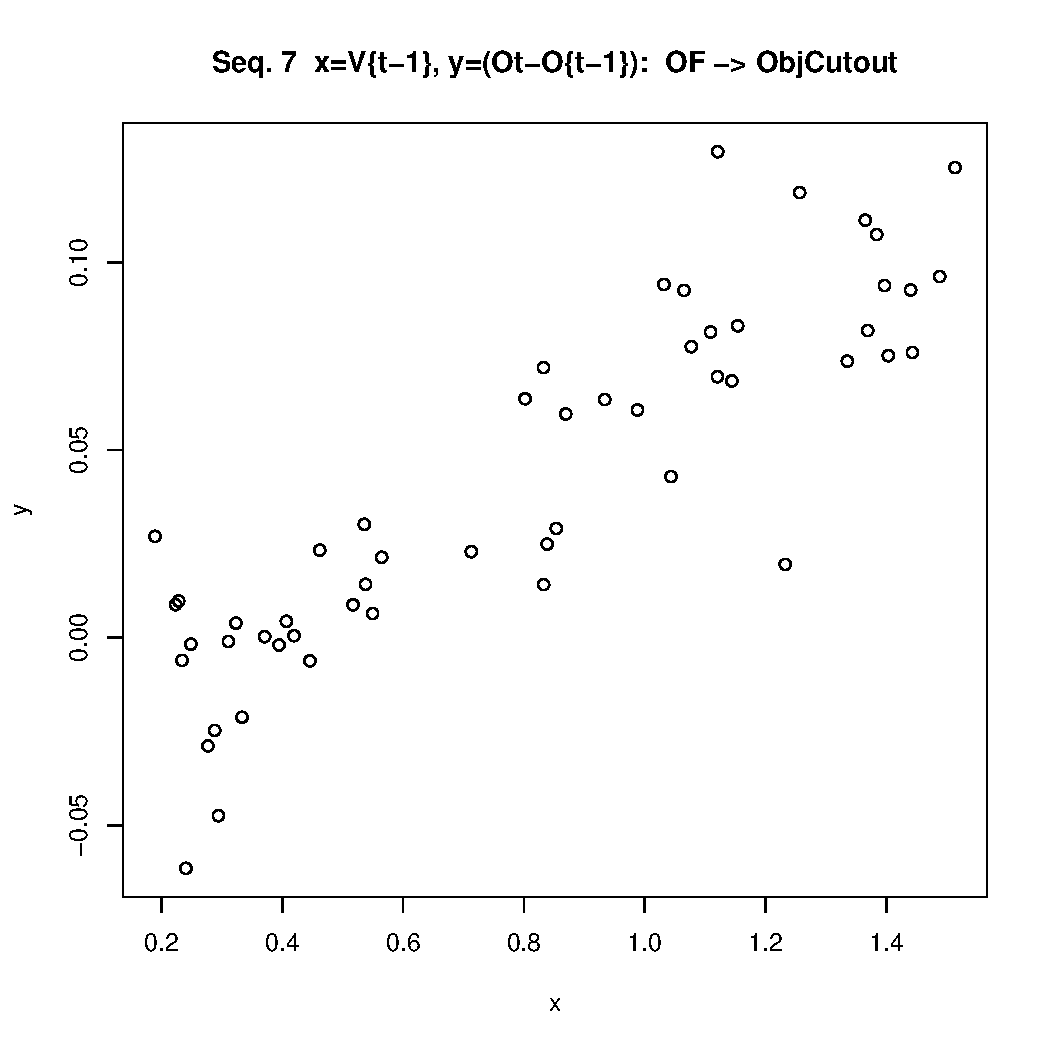
\includegraphics[width=60mm]{figures/DaimlerOBJplotSerie7.pdf}&
    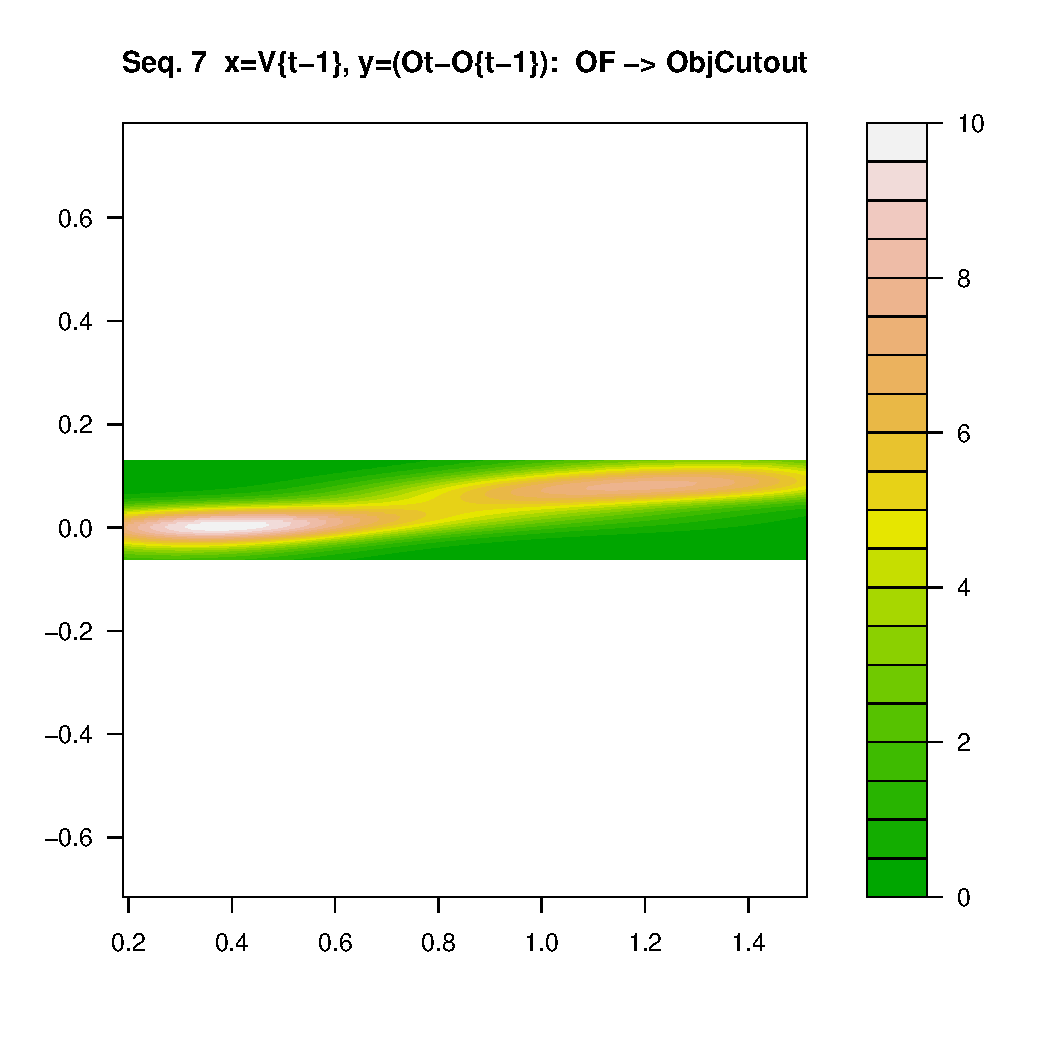
\includegraphics[width=60mm]{figures/DaimlerOBJcontourSerie7.pdf}\\
  \end{tabular}
      \caption{ \label{Figure:daimlerVvsOffs}Time and contour plots attesting the linear correlation between $V(t-1)$ vs $O(t) - O(t-1)$.}
\end{figure}

Finally, Figure \ref{Figure:daimlerLEdynGeneric} presents a rough overview of the final structure of the dynamic OOBN\footnote{Full details can not be provided for confidentiality reasons, but will be included in the confidential Deliverable 6.1.}. It illustrates how the temporal connection is only made on the top nodes (i.e., S\_REAL) involving the situation-features in consecutive time steps\footnote{Although for the sake of clarity in the representation the sensor measurement structure is only shown for S\_REAL$_1$, this is identical for all sensor variables.}. The final event or manoeuvre prediction is then determined by the combination of all possible hypotheses ($Hypothesis_1, \ldots, Hypothesis_n$). There exist hypotheses at the top level that correspond to each of the sensor measurements, and then other different layers of hypotheses that combine the different outcomes till the final event, forming a polytree structure. %and the position of the OBJ with respect to the EGO car.

Similarly to the static OOBN, if we modelled V\_LAT\_REAL and O\_LAT\_REAL as continuous variables, the conditional probability distribution of the LE hypotheses given the V\_LAT\_REAL and O\_LAT\_REAL variables would not fall in the conditional linear Gaussian family \cite{JensenNielsen2007}, because we would have discrete children with continuous parents. Once again, the pursued approach to deal with this problem is the discretization of the V\_LAT\_REAL and O\_LAT\_REAL variables (hence, they are represented with a green color in Figure \ref{Figure:daimlerLEdynGeneric}). Since the remaining continuous variables S\_MEAS and S\_SIGMA are always observed, all the inferences can be implemented only over discrete potentials.

\begin{figure}[ht!]
\begin{center}
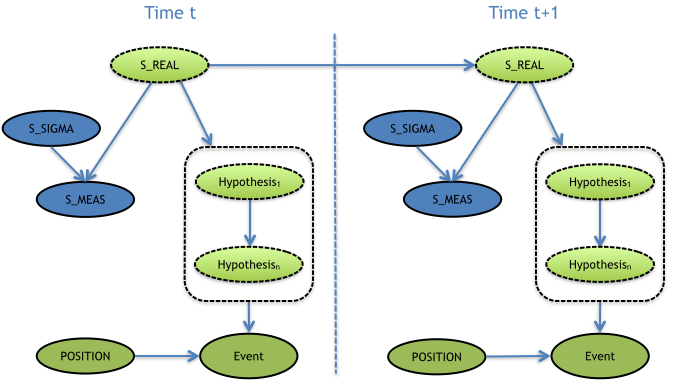
\includegraphics[scale=0.49]{./figures/DaimlerLEdynGeneric}
\end{center}
\caption{\label{Figure:daimlerLEdynGeneric}Daimler dynamic OOBN model with several hypotheses. Although for the sake of clarity in the representation the sensor measurement structure (i.e. S\_MEAS and S\_SIGMA) is only shown for S\_REAL$_1$, this is identical for all sensor variables. S\_REAL variables are plotted in green color to highlight that they are discretized, because otherwise we would have a model with continuous parents and discrete children.}
\end{figure}

%A DBN induces a number of constraints on the compilation of the network into a computational structure. One constraint relates to transferring the belief state from one time slice to the next where the belief state is the probability distribution over the variables shared by neighbouring time slices. In general, the belief state is transferred as a joint distribution. We have imposed limitations in our dynamic model so that the next state depends only on the current state, and not on the sequence of events that preceded it, i.e. first order Markov model. Although in principle this might seem as a strong limitation, we have reasons to believe that this property might hold in our data. Fig. \ref{Figure:daimlerCorrel} displays, at the top, the sample correlograms for lateral velocity and offset, that is, the correlation of the data with lagged values of themselfves. The partial correlogram (bottom figures) is used to remove the common linear effect of the data in between samples. In our example, for both variables, the correolograms take some time to decay to zero, while the partial correlograms are large for lag one and then small of all other lags. This indicates that the correlation between non consecutive samples is due to the common relationship of these samples and the samples in between \cite{Newton:1988}.

%--------------------------------------------------------------------------------------------------------------------
\subsubsection{Earlier prediction of the need for a lane change based on relative dynamics}
%--------------------------------------------------------------------------------------------------------------------

Earlier prediction of manoeuvre intentions could be achieved before any development of the trend for lateral evidence has been observed. A first indication of possible lane change intention could be detected through the relative dynamics between one vehicle (e.g., EGO) and the vehicles in front of it on the same lane. For instance, if a vehicle is driving slowly in front of the EGO vehicle on the same lane, this may indicate a need for a lane change. In fact, in order to continue its safe driving, the EGO vehicle should either break and reduce its speed to the speed of the vehicle in front, or alternatively, change to the adjacent lane, if the neighbour lane is free and no other vehicle is approaching with a higher speed. 

A continued safe manoeuvre (of type ``lane follow'' or ``lane change'') is modelled by estimating the time to collision (TTC) with a vehicle in front (on the same lane) or eventually with an approaching vehicle (on the neighbour lane). For a safe manoeuvre, TTC should be higher than $1$ second, either when the EGO vehicle wants to change to the neighbour lane or needs to break to ensure safe driving on the same lane. We assume that using this approach will further enhance the prediction horizon for manoeuvre recognition (up to $5$ seconds).

Similarly to the models described in Figure \ref{Figure:daimlerLEdyn}, a new dynamic OOBN is defined with the hypothesis ``relative dynamics'' (REL\_DYN), as shown in Figure \ref{Figure:daimlerreldyn}.  Due to confidentiality reasons, we can not give at this stage of the project further details about this model (full details will be given in the confidential Deliverable 6.1.).

%We can see however that this model have the same general structure that the dynamic models proposed for the previous application scenario. 
% any type of data analysis that supports this hypothesis.
 
\begin{figure}[ht!]
\begin{center}
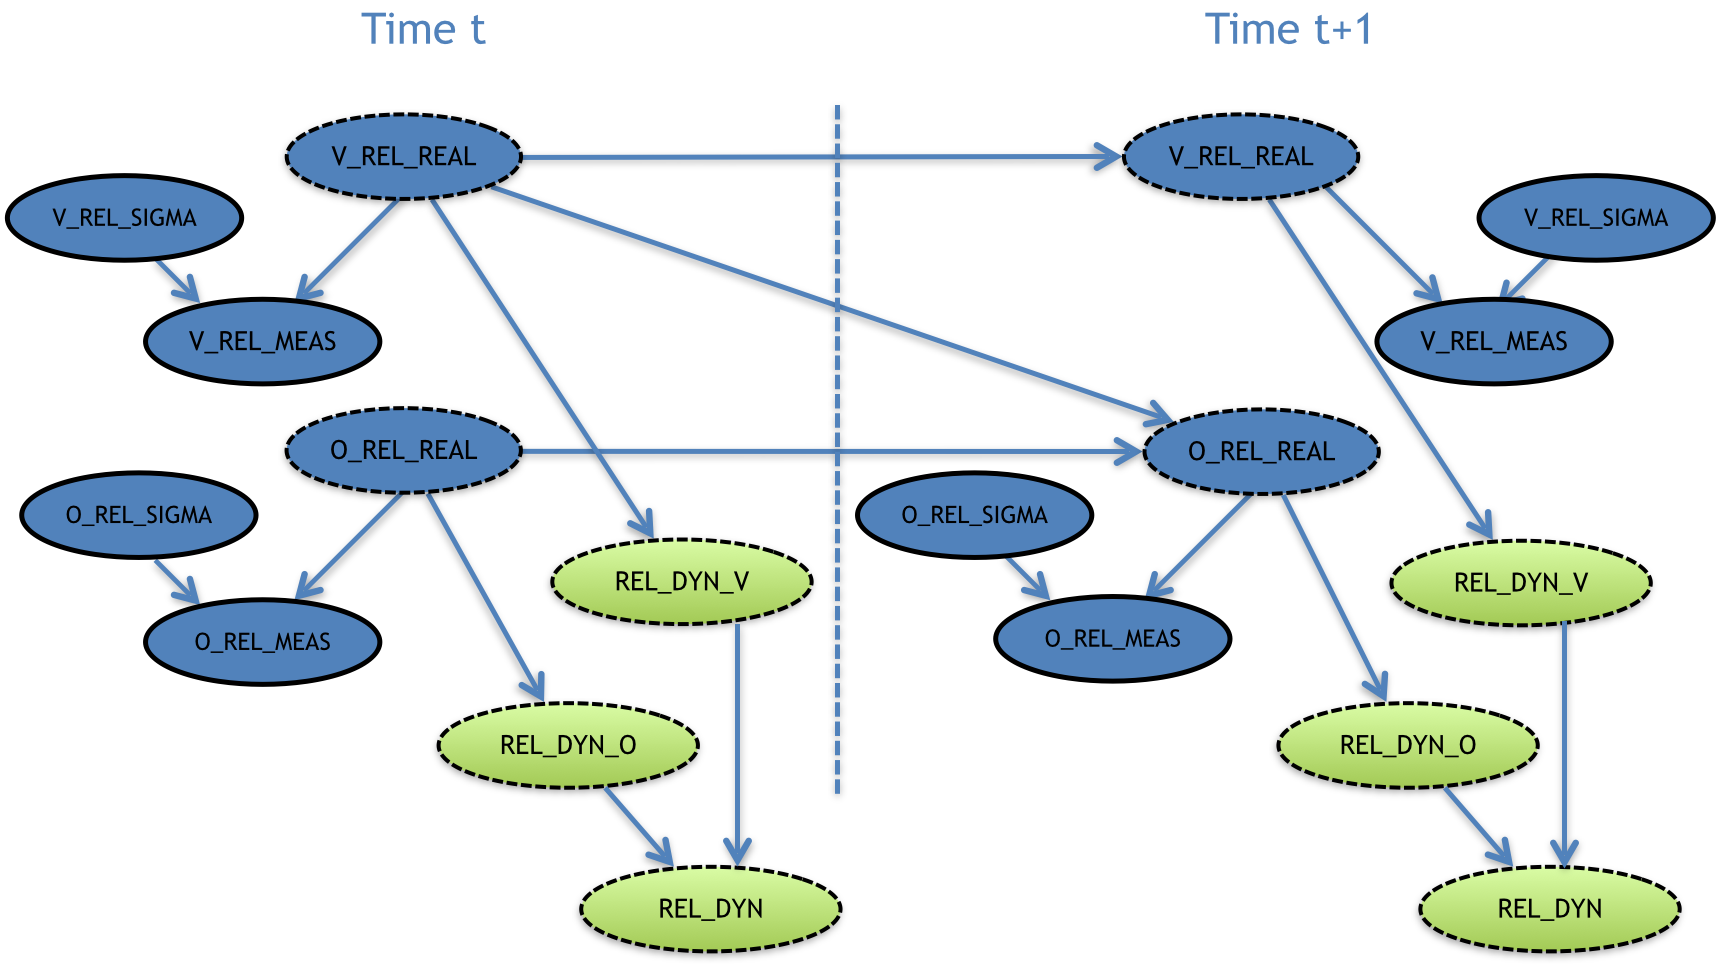
\includegraphics[scale=0.48]{./figures/Daimlerreldyn.png}
\end{center}
\caption{\label{Figure:daimlerreldyn}Daimler dynamic OOBN model with relative dynamics. V\_REL\_REAL and O\_REL\_REAL refer to the relative velocity and relative distance between the EGO and the car in front, respectively. The other variables with \_MEAS and \_SIGMA suffixes refer to the measured values and the uncertainty of the measurements, respectively, as commented in the previous section for other sensor readings.}
\end{figure}


%This BN fragment  models the hypothesis REL\_DYN with 3 states Left/Follow/RIGHT, utilising the independency assumption for the discrete variables V\_REL\_MEASSURED and X\_REL\_MEASSURED.
%
%If we compare the structure of this network with that of Figure \ref{Figure:daimlerLEdyn}, we can observe two additional nodes:  REL\_DYN\_V\_REL\_OBJ and REL\_DYN\_X\_REL\_OBJ. They are the results of a modelling trick to simplify the EM-learning of parameters from data for the static BN fragment.
%
%\textcolor{red}{Note that the new REL\_DYN hypothesis introduced would require two instances in the OOBN, one for the relative dynamics of the EGO with the OBJ in front, and another one for the OBJ and another OBJ in front of it. Each REL\_DYN would indicate if the EGO and the OBJ cars are going to turn right, left or continue straight.}
%

%--------------------------------------------------------------------------------------------------------------------
\subsubsection{Discussion and future models}\label{subsubsection:daimlerfuture}
%--------------------------------------------------------------------------------------------------------------------

The above included proposals are preliminary models designed in line with the expert knowledge facilitated by Daimler. They all try to balance a good level of expressiveness and efficiency during inference. However, in any case, they should only be seen as first proposals that might be modified/adapted in the future if they do not meet the efficiency and accuracy targets specified in the requirements \cite{Fer14}. 

For application scenario 1 (see Section \ref{Section:Daimler:EarlyRecognition}), we envision, for example, the possibility of considering not only the temporal dependences between consecutive time steps for the sensor measurements but also, or instead, consider the temporal links between hypotheses at consecutive time-steps (i.e., adding in Figure \ref{Figure:daimlerLEdynGeneric} temporal links between hypotheses nodes at different time-steps). It seems natural, for instance, that the probability of the EGO lateral evidence would be higher given its lateral evidence at the previous time-step. The same applies for the remaining hypotheses, such as TRAJ, OCCGRID, and the final hypothesis or event that identifies the type of manoeuvre. However, adding these type of dependences would greatly increase the complexity of inference in the resulting dynamic OOBN, because the total number of dependencies will be much higher over time. As described in D1.2 \cite{Fer14}, models in this case are subject to very strong constraints in terms of computational efficiency, so we should be very cautions at this respect. 

Another possible extension is to consider an extra hidden variable to model the acceleration in the dynamic OOBN model. We believe that assuming that lateral velocity varies according to a constant acceleration can lead to inaccuracies. Figure \ref{Figure:daimlerVel} (a) shows the behaviour of lateral velocity (V\_Lat) for a randomly selected sequence which corresponds to an EGO-CutIn manoeuvre. At the beginning of the sequence, acceleration is close to zero, however, approximately between time-steps 30 and 50, a higher acceleration value should be taken into account. The contour plot on Figure \ref{Figure:daimlerVel} (b) shows a large density of points around lower and higher values of $V$ where the acceleration is constant, but just isolated points in between. Hence, we think that the dynamic model could benefit from an extra hidden variable to represent acceleration (A\_Lat) as displayed in Figure \ref{Figure:tempDynAccel}. The following equation would be then considered for velocity at consecutive time steps: %(SIGMA and MEAS. variables have been left out for simplicity). 

\begin{equation}
V(t) =V(t-1) +A(t-1)dt +\epsilon
\end{equation}

\noindent where $A(t-1)$ denotes the acceleration at time step $t-1$ and $\epsilon$ is a white noise. In this model, acceleration is assumed to be almost constant between two consecutive time steps, i.e., $A(t) = A(t-1) + \epsilon$. 

\begin{figure}[ht!]
  \centering
  \setlength{\tabcolsep}{0.05pt}
  \renewcommand{\arraystretch}{0.02}
    \begin{tabular}{cc}
    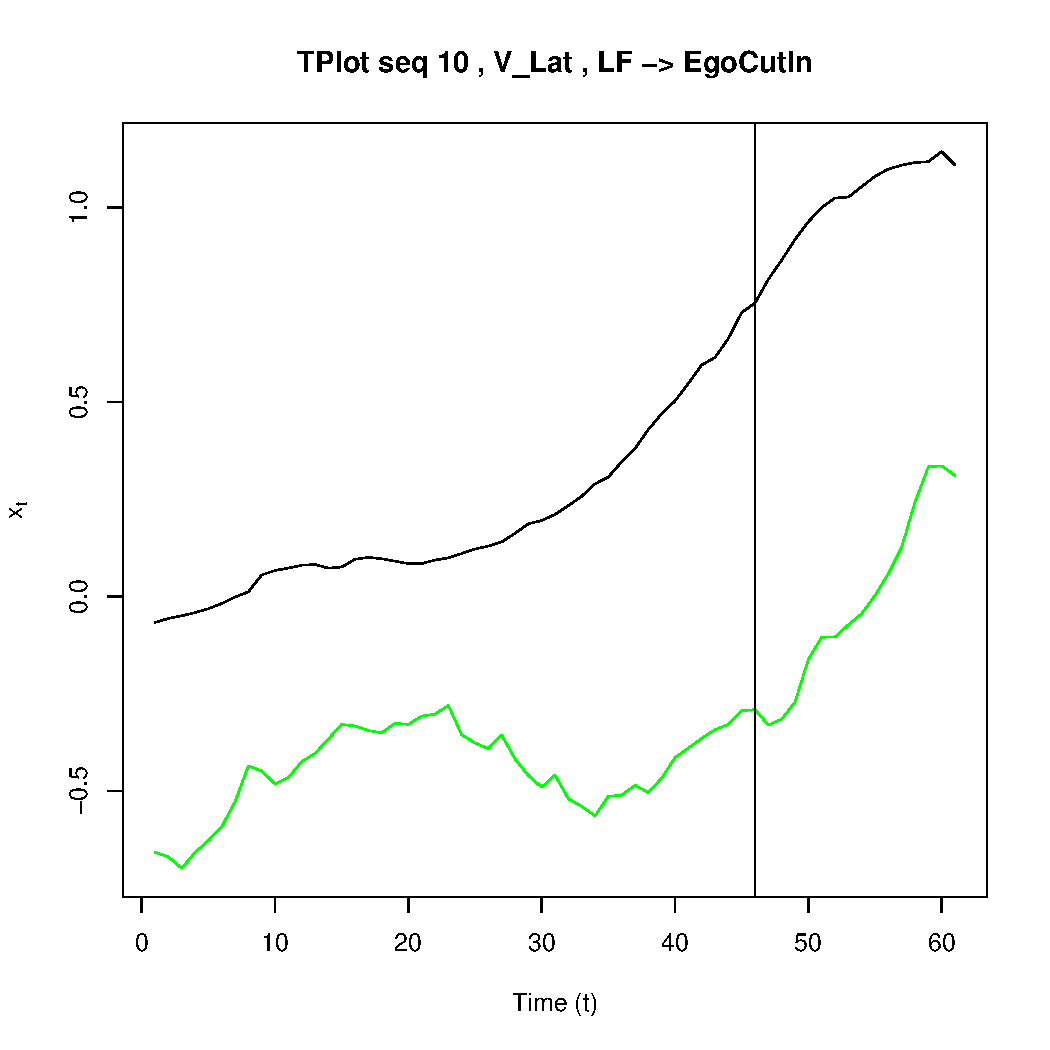
\includegraphics[width=60mm]{figures/DaimlerLE_EGO_L_LE_OBJ_R_EGOCutInVel.pdf}&
    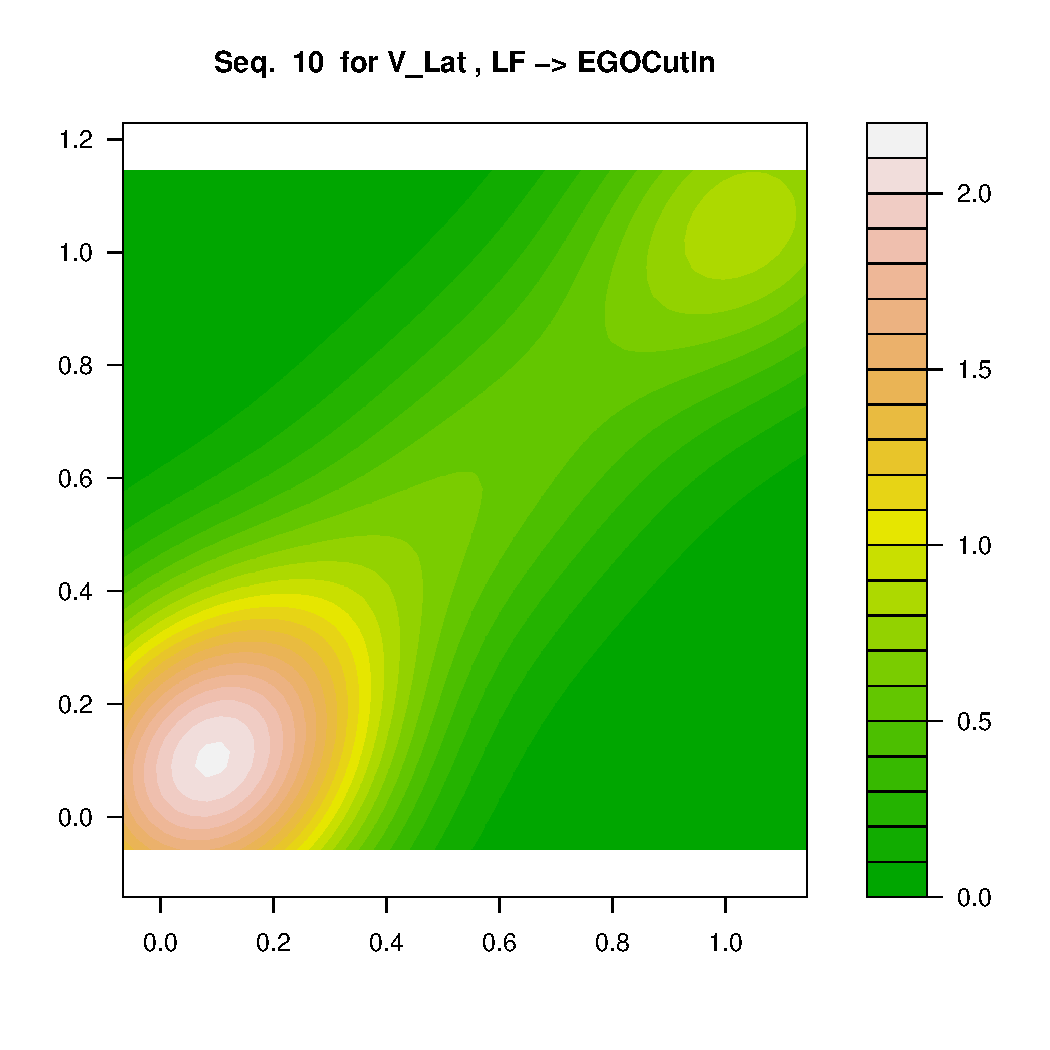
\includegraphics[width=60mm]{figures/DaimlerBivariate_temporal_analysisEGO_LVel.pdf}\\
  \end{tabular}
      \caption{ \label{Figure:daimlerVel}Time and contour plots for $V(t)$ versus $V(t-1)$ showing that modelling the acceleration should be considered to capture the variations in the data.}
\end{figure}

\begin{figure}[ht!]
\begin{center}
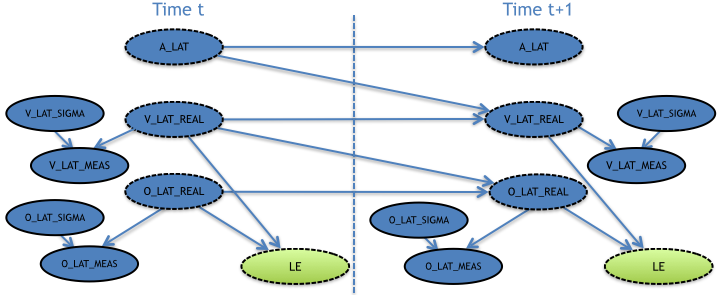
\includegraphics[scale=0.48]{./figures/DaimlertempDynAccel}
\end{center}
\caption{\label{Figure:tempDynAccel}Daimler dynamic OOBN fragment for the LE hypothesis with a hidden node for acceleration (A\_Lat).}
\end{figure}

%!TEX root = D2.1_AMIDSTModellingFramework.tex

\newpage
\newpage
\newcommand{\X}{\mathbf{X}}
\newcommand{\Y}{\mathbf{Y}}
\newcommand{\Z}{\mathbf{Z}}

\subsection{CajaMar Models}
\label{Section:CajaMarModels}

\subsubsection{Introduction}

There are two tasks to be solved for Cajamar's use case (see D1.2 and DoW). The main one is
the estimation of the \emph{probability of default}, defined as the probability that a
credit operation will end up in default within two years. The secondary task consists in obtaining 
good customer profiles in terms of risk, so that marketing campaigns can be
specifically targeted to these low risk customers. 

%%%%%%%%%%%%%%%%%%%%%%%%%%%%%%%%%%%%
\subsubsection{Predicting probability of default}
\label{SubSection:Predicting}
%%%%%%%%%%%%%%%%%%%%%%%%%%%%%%%%%%%%

%---------------------------------------------------------------------------------------------
\subsubsection*{Introduction of the problem} 

In any commercial bank, every time a customer applies for a loan, the bank experts evaluate the customer's risk profile before making their decision. 

At Cajamar, this risk evaluation protocol is implemented by evaluating whether the client is going to default or not within the following two years. When a client is labelled as defaulter, he/she will remain defaulter in the database at least two more years, so the client will become non-defaulter again when everything has been paid appropriately during the last 2 years. 

The problem of predicting the customer risk of default is currently addressed at Cajamar by an automatic supervised classification model (i.e. a logistic regression). It takes information about the recent financial activity of a customer, as well as information about recent past paying behaviour provided by other Spanish financial institutions. Finally, using this information, predictions about the probability that the client will default during the following two years are made. The methodology currently employed does not assume dependence structure among the variables and current predictions are made using only a set of $27$ variables out of more than $1000$ available. Updates in risk predictions are made on a monthly basis, whereas the predictive model is only updated after several years. These low update frequencies are partly due to limitations in the available commercial software and the computing resources.

The objective is to daily update the risk of default for every customer of the bank. This daily evaluation will be made by creating two data sets: the model training data set and the model evaluation data set (see Use Case 1 in D1.2). How these data sets are created gives us some insights about the nature of this risk prediction problem.  Figure~\ref{Figure:CajaMarTimeLine} show how the evaluation and training datasets are generated within a time-line. The current time is denoted as $t$ and the time $2$ years back as $k$, i.e., $k=t-2$ years. 

\begin{figure}[htbp]
\centering
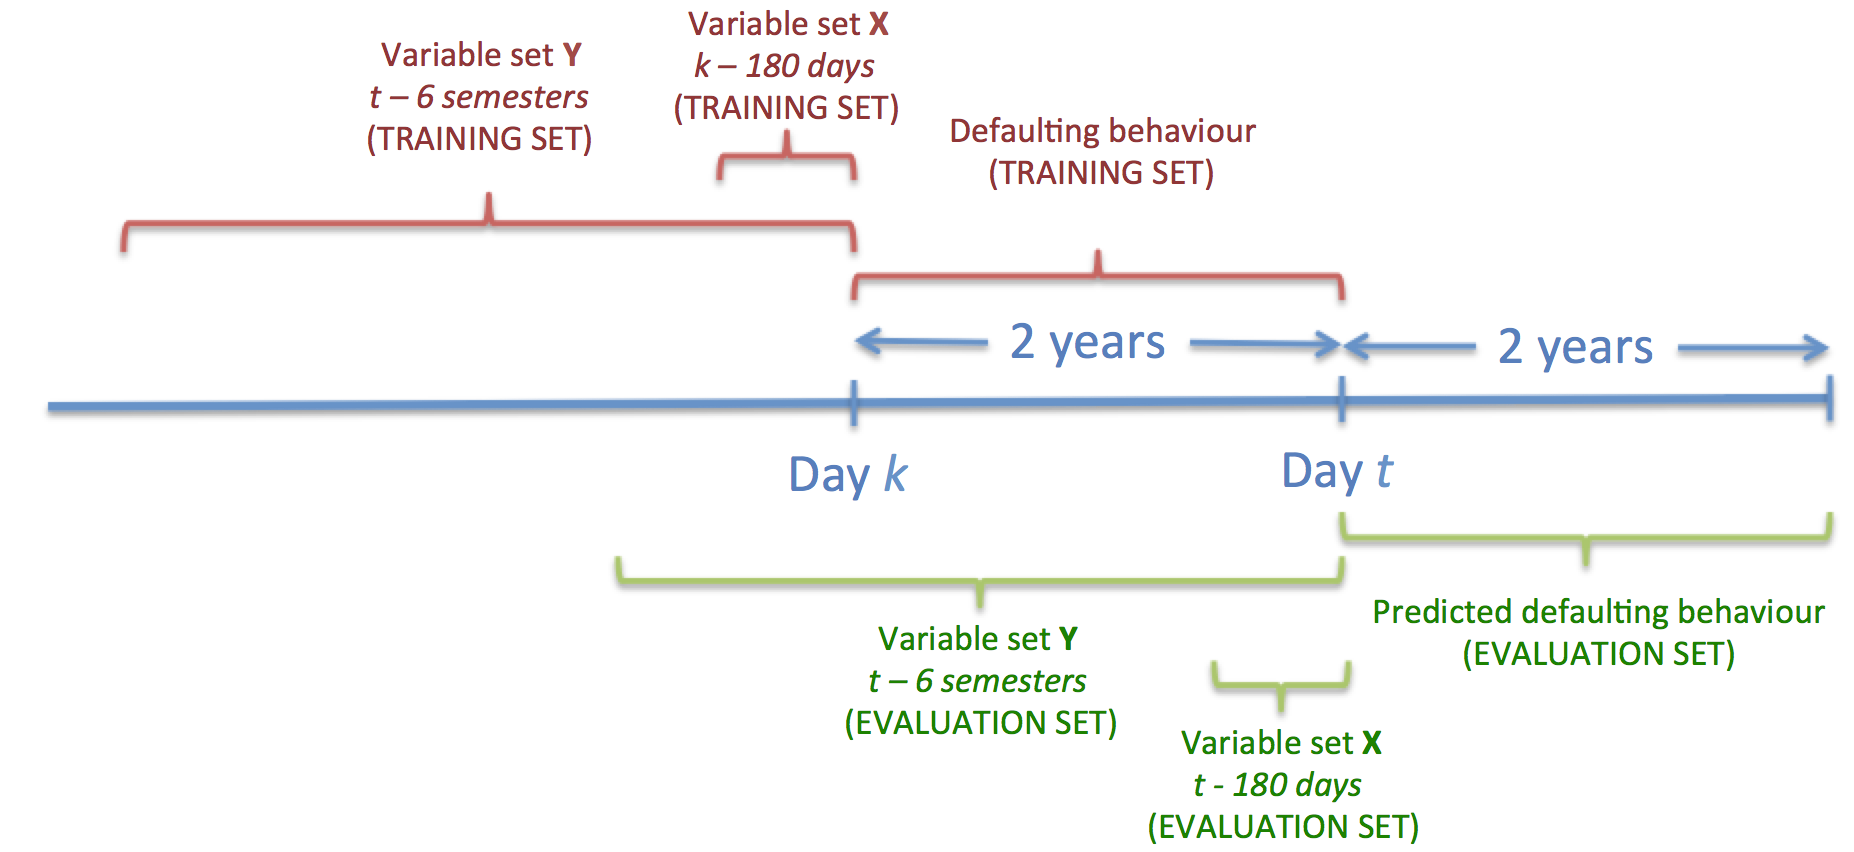
\includegraphics[scale=0.4]{figures/CajaMarTimeLine}
\caption{\label{Figure:CajaMarTimeLine}Time-line showing how the evaluation and training data sets are generated.}
\end{figure}

\begin{itemize}
\item \textbf{Model Evaluation Data Set:} The evaluation data set is created at time $t$. This data set contains a record for every client to be evaluated. Note that, data about the predicted defaulting behavior is still missing at time $t$ when conforming the evaluation dataset. It will be obtained after performing inference on the model. As in any standard evaluation data set in supervised classification settings, each record will contain the values of the predictors variables for this customer. The predicting variables refers to the financial activity and the paying behaviour of the customers in a recent past, and their socio-demographic data. 

The recent {\bf financial activity} of a customer refers to attributes such as ``account balance'', ``number of credit card operations'', etc. in the last 180 days\footnote{This limit is fixed by the Bank of Spain}. These attributes usually change daily for a customer, so they are encoded by introducing a set of variables for each attribute, one for each day back from current time $t$. Hence, the financial activity of a customer is specified by a number of variables equals to 180 times the number of predictors. 

In the case of {\bf past paying behaviour}, the attributes refers to variables such as payments inside Cajamar (loans, mortgages, credits, etc.). A record of the last 36 months divided by semester is considered when building the evaluation data set. So, a number of variables equals to $6$ times the number of attributes referring to the paying behaviour are used in this case. Moreover, some other static variables with information about payments to other financial institutions or companies (phone and electricity bill, public bodies, etc.) is included in this group of variables.

The dataset for the evaluation of customers is detailed in Table~\ref{tab:EvaluationDataset}. Note that there exist another group of variables denoted as $\Z$ (mainly sociodemographic variables) that are not replicated over time as they remains fixed. 
%The data included in both data sets regarding these variables refer to time $t$.


\begin{table}[htbp]
\centering
\begin{tabular}{c|ccc|ccc|c}
	&\multicolumn{3}{c|}{Days} & \multicolumn{3}{c|}{Semester} \\
     Time $t$              & $\X^{(t-180)}$ & $\ldots$ & $\X^{(t-1)} $ & $\Y^{(t-6)}$  & $\ldots$ & $\Y^{(t-1)} $ & $\Z$  \\  
\hline
Client$_1$  &                                                  &              &                     &                               &                     &        \\ 
$\vdots$      &                                                 &               &                     &                                &                     &      \\ 
Client$_n$  &                                                &               &                     &                                &                     &     \\ 
\end{tabular}
\caption{Evaluation dataset at time $t$. Attributes for financial activity, paying behavior and sociodemographic information are denoted as $\X$, $\Y$ and $\Z$, respectively.}
\label{tab:EvaluationDataset} 
\end{table}

In conclusion, the idea is to take each of the records (i.e. customers) of this data set and compute the probability of defaulting within the following two years. Finally, the risk table in the system is updated (see Table~\ref{tab:riskTable}).

\begin{figure}[h]
\centering
\begin{tabular}{c|ccc|ccc|c}
     Time $t$  & Risk of defaulting \\  
\hline
Client$_1$  &    $r_1$  \\ 
$\vdots$      &   $\vdots$   \\ 
Client$_n$  &   $r_n$  \\ 
\end{tabular} 
\caption{Table containing the risk of defaulting for every client.}
\label{tab:riskTable}
\end{figure}


If at some point the probability of defaulting of some customers rises above some predefined threshold, the bank considers taking preventive actions to reduce the chances of defaulting by the customer.

\item \textbf{Model Training Data Set:}  The training data set is built in the same way as the evaluation data set. They contain the same set of predictive variables plus the \emph{Defaulter} variable. The main difference is they refer to different time points. The predictive variables in the evaluation data set are built from time $t$ (current time) backward, whereas the ones in the training data set are built from time $k$ (2 years before $t$) backward. The dataset for training/updating the model is detailed in Table~\ref{tab:TrainingDataset}.
\begin{table}[h]
\centering
\begin{tabular}{c|ccc|ccc|c|c}
	&\multicolumn{3}{c|}{Days} & \multicolumn{3}{c|}{Semester} & \\
     Time $t$              & $\X^{(k-180)}$ & $\ldots$ & $\X^{(k-1)} $ & $\Y^{(k-6)}$  & $\ldots$ & $\Y^{(k-1)} $ & $\Z$ & Defaulter$^{(t)}$\\  
\hline
Client$_1$  &                                                  &              &                     &                               &                     &        &  \\ 
$\vdots$      &                                                 &               &                     &                                &                     &       & \\ 
Client$_n$  &                                                &               &                     &                                &                     &     & \\ 
\end{tabular} 
\caption{Training dataset at time $t$ with $k=t - 2$ years.  The notation is the same as in Table~\ref{tab:EvaluationDataset}.}
\label{tab:TrainingDataset} 
\end{table}

Unlike the evaluation data set, each record contains a class label indicating if this customer is defaulter o non-defaulter as predicting variables data are prepared in such a way that information about defaulting behavior is available at time $t$. To decide if a customer is defaulter or not, we look at the data 2 years back from current time $t$. If during these two years there are not any evidence of defaulting and the client's payments (at Cajamar and other financial institutions) has gone as expected, the client is labelled as non-defaulter. Otherwise, it is labelled as defaulter.

\end{itemize}

Next, we propose two modeling solutions for the risk prediction problem.



\subsubsection*{Static Model} 

In this first approach we do not explicitly consider some of the dynamics of the problem: we do not model that a customer can be non-defaulter and defaulter at different moments in time (e.g. one customer can be creditworthy and, after some time, go bankrupt due to unemployment). Instead, we consider a static prediction model where given the financial behaviour of the client over a recent past, it predicts whether the client will default or not within the next 2 years. Similarly to what it is done in the current Cajamar approach. 

Figure \ref{Figure:CajaMarStatic} shows the general structure of this static model. The payment variables are grouped by semesters whilst the financial activity variables by day. Note that past sociodemographic information are not necessary as it does not change frequently.
%For the sake of simplicity, for now on and in the graphical models depicted, we do not explicitly show the variables that refer to monthly information during the last 36 months. 

\begin{figure}[htbp]
  \centering
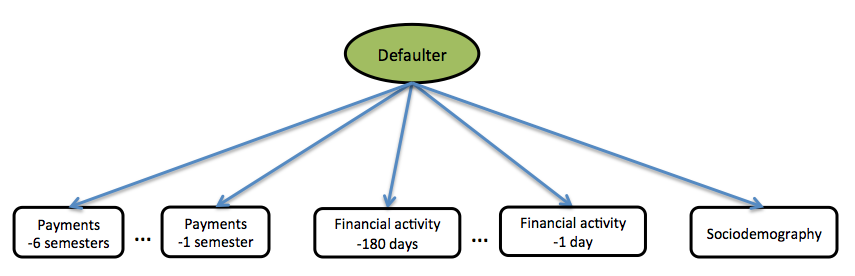
\includegraphics[scale=0.5]{./figures/CajaMarModel0}
\caption{\label{Figure:CajaMarStatic}Global structure of the static model. Each white box represents a set of variables for a particular time. The green node on top is the class variable \emph{Defaulter} that represents the probability that a customer will default within the next two years. } 
\label{fig:static}
\end{figure}

Expert knowledge from the bank point out that predicting variables are expected to be related so they might be connected within each box (e.g. according to a tree structure and, globally, conforming a TAN). 




%Figure~\ref{fig:CajaMarBayesianNetwork} shows a Bayesian network structure learnt from customers data that have been aggregated from different times, e.g., 180 times for financial activities \textcolor{red}{(We think it has no influence to get more dependences in the network structure)}
%To computationally simplify this learning in this preliminary overview,  \textcolor{blue}{only data correspond to one day?} are considered, meaning that the number of cases for learning has been considerably reduced. 
%Looking at the structure is evident that indeed there exist dependences between some of the variables\footnote{For confidentially reasons variable names are not shown}. The structure has been learnt using the R package \texttt{bnlearn}~\cite{Scu10, Nag13}.
%
%\begin{figure}[htbp]
%  \centering
%    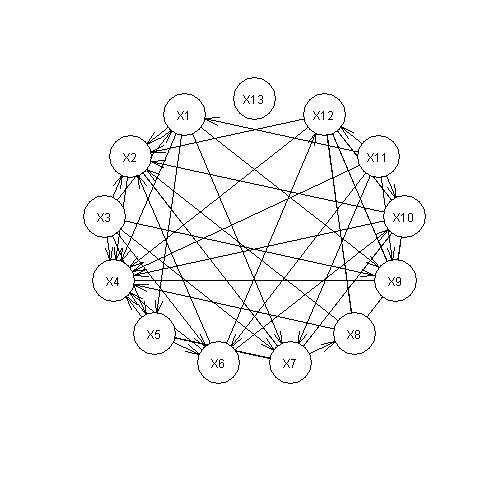
\includegraphics[width=70mm]{figures/CajaMarBayesianNetwork}
%    \vspace{-1cm}
%    \caption{Bayesian network structure learnt from 13 variables randomly chosen from the whole set of variables.}
%    \label{fig:CajaMarBayesianNetwork}
%\end{figure}


%
%
%\begin{figure}[htbp]
%  \centering
%    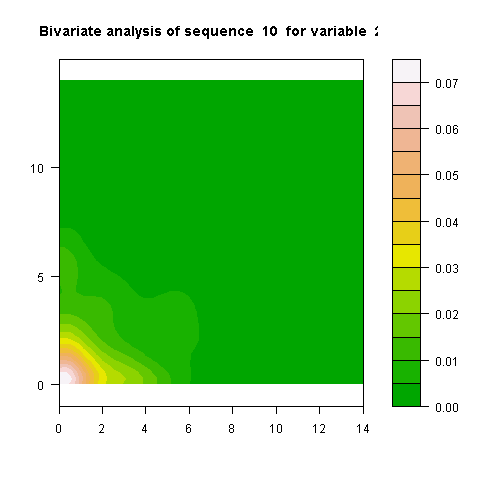
\includegraphics[width=70mm]{figures/CajaMarbv4}
%    \caption{Contour plot with (ideally) strong linear correlation between two variables \textcolor{blue}{(maybe class-conditioned?).}}
%    \label{fig:CajamarContourPlot}
%\end{figure}



%Figure \ref{fig:CajamarContourPlot} shows the contour bivariate plot for two variables, showing a clear linear relationship between them. 
Moreover, it may happen that one variable is even a replica of the other or contain quite similar information
%This might even indicate that one variable is just a replica of the other or contain quite similar information, 
and their joint contribution will not only make learning and inference computationally more expensive, but it could lead to poorer performance. This would contribute to support the need to explore suitable feature selection techniques as specified in Use Case 2 of Cajamar's Requirement analysis\cite{Fer14b} .



It is also of major interest to analyse the type of density probability distributions to use in the proposed model. Figures \ref{Figure:cajamarMixt} shows the density histogram for the values of one continuos attribute for defaulters and non-defaulters respectively. The density curves represent a credible approximation using mixture of Gaussian distributions, which is the case for most of the other predictive attributes. Note that for defaulters, the values of the \emph{end-of-day balance} are overall lower compared to those corresponding to non-defaulters.

\begin{figure}[htbp]
  \centering
    \begin{tabular}{cc}
    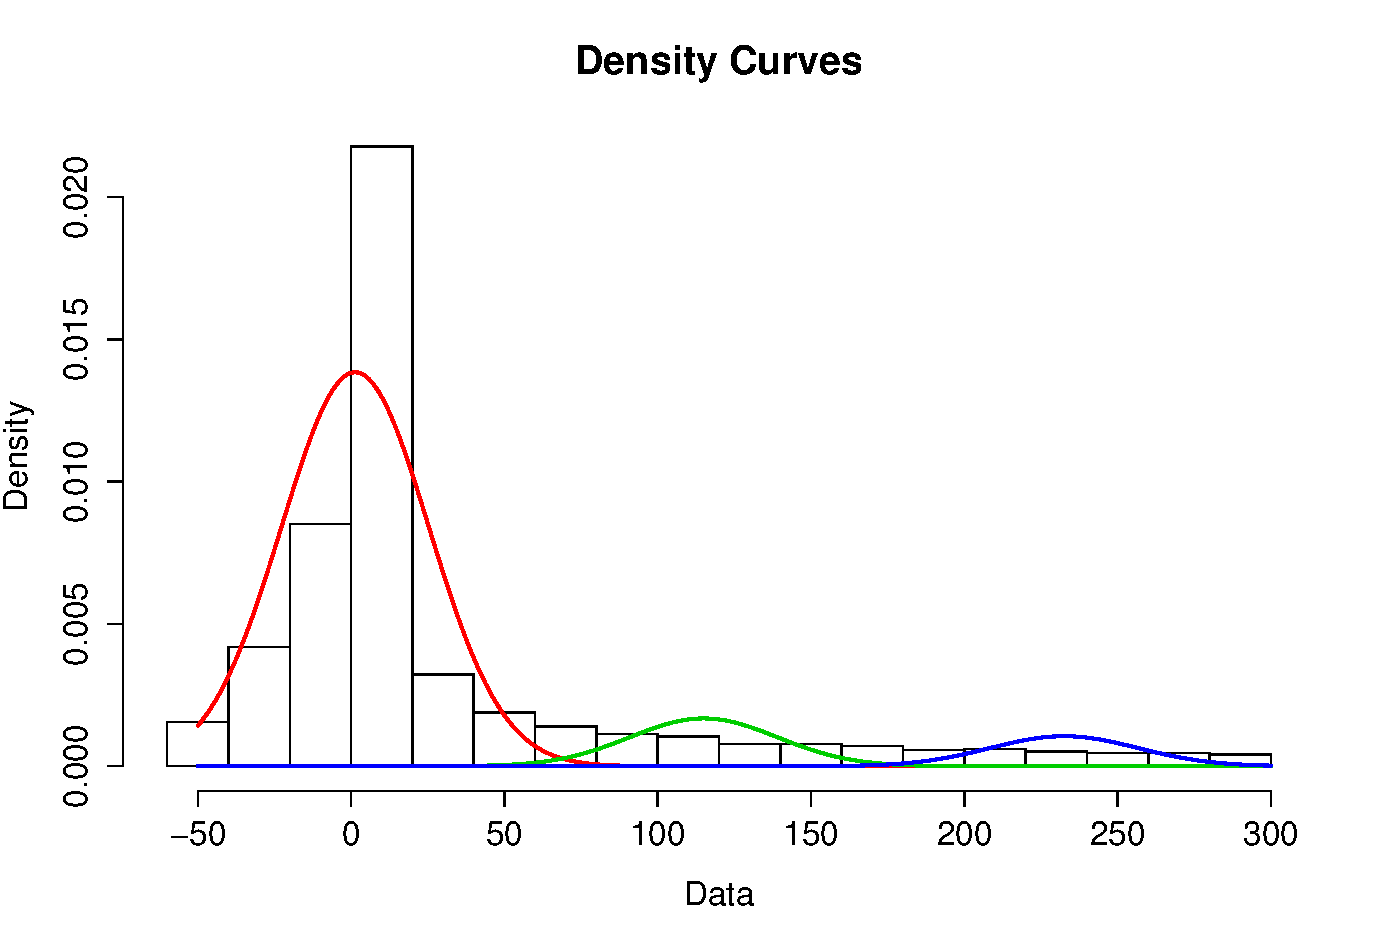
\includegraphics[width=70mm]{figures/CajaMarmixtureBalanceDef}&
    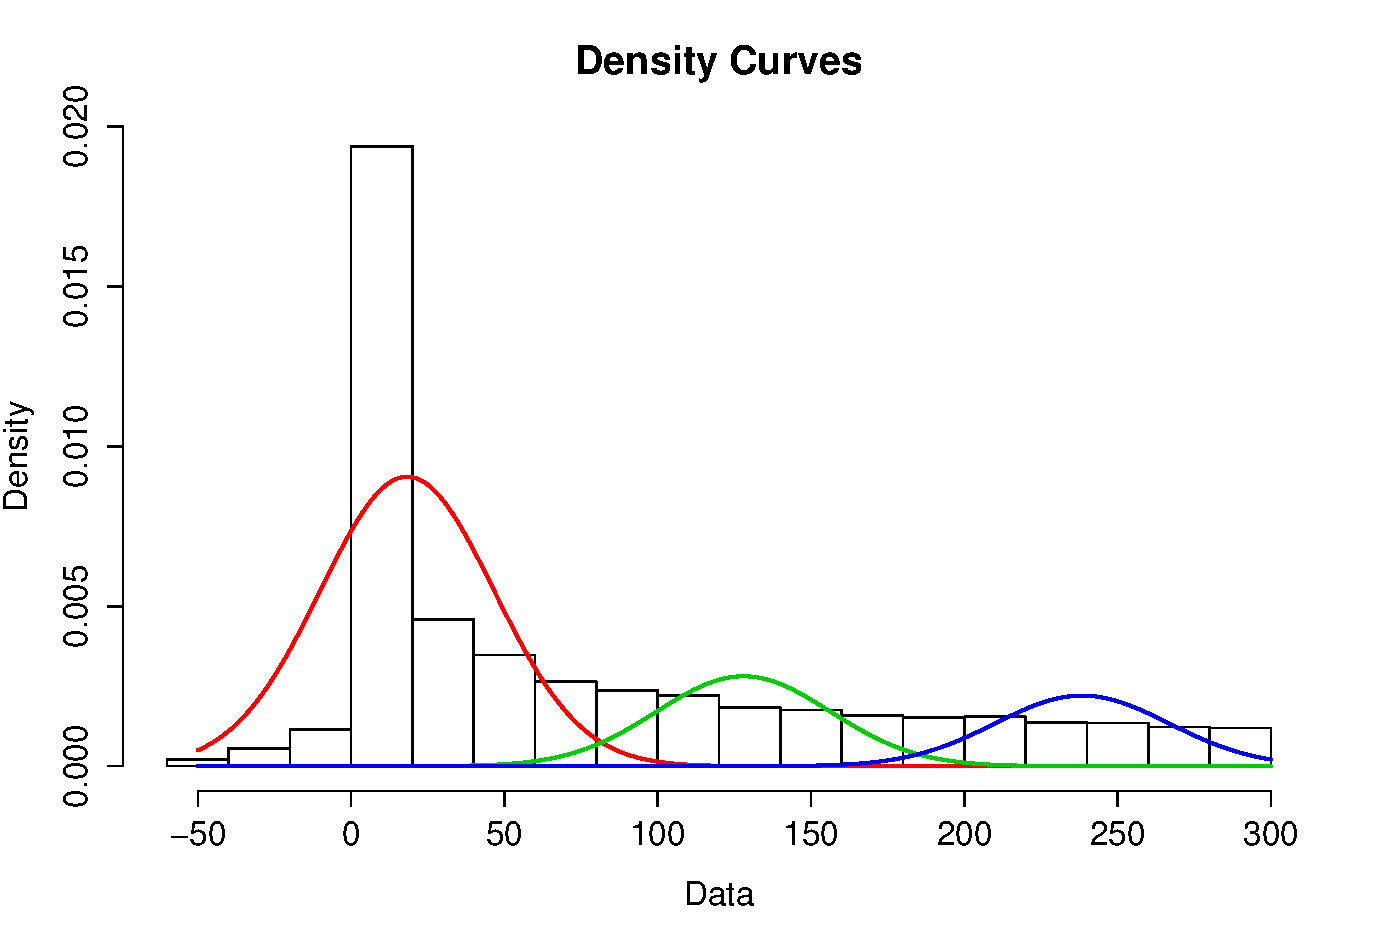
\includegraphics[width=70mm]{figures/CajaMarmixtureBalanceNonDef}\\
  \end{tabular}
    \caption{\label{Figure:cajamarMixt}Mixture of Gaussian approximation of one predicting variables conditioned to defaulter (left) and non-defaulter (right) value of the class variable.}
\end{figure}

There exist however discrete (non-ordinal) predictive attributes which impose a limitation in the structure of the Conditional Gaussian network, since discrete attributes cannot have continuous parents. This might not be a problem for the semi-naive Bayesian network to be considered, and it is certainly not a problem for naive Bayes. Nonetheless, if this limitation were found to be problematic, then other probability distributions families will be explored, such as Mixture of Truncated Basis Functions~\cite{Lan12}, which can cope with any generic model structure. 

In summary, the process of building this static model consists of the following steps:

\begin{enumerate}
\item Using a set of SQL queries over the main relational dataset, a single flat table containing the information for training the model (see Table~\ref{tab:TrainingDataset}) is constructed every day. Note that, for instance, for variables related to financial activities, training data between two consecutive days $t$ and $t+1$ only differ in the new data arriving at day $t+1$ and obviating the data from 180 days ago at day $t$. Similar idea is applied for the paying behaviour variables.
\item Update the existing Bayesian network classifier with the new data.  Although relationships are more common between variables within each box, dependences among variables in different boxes are also allowed. 
\item Construct a single flat table with latest information about customers (evaluation dataset) in order to compute the latest risk profiles. This dataset was depicted in Table~\ref{tab:EvaluationDataset}.
\item Update the risk in Table~\ref{tab:riskTable} for every customer by propagating each record from the evaluation dataset in the static classifier obtained in Step 2. 
\end{enumerate}


%\begin{figure}[ht]
%\begin{center}
%\begin{tikzpicture}[->,>=stealth,shorten >=1pt,auto,node distance=2cm,semithick,
%        amarillo/.style={fill=yellow,rectangle,draw},
%        rojo/.style={fill=red,rectangle,draw,rounded corners}]
%        \node[green] (default) {Default};
%        \node (dot) [below of=default] {$\cdots$};
%        \node[amarillo] (tran1) [left of=dot] {Day -180};
%        \node[amarillo] (tran180) [right of=dot] {Day -1};
%        \draw (default) to (tran1);
%        \draw (default) to (tran180);
%\end{tikzpicture}
%\end{center}
%\caption{\label{Figure:CajaMarStatic}Global structure of the static model. Each yellow box represents a set of variables measures during the same day.
%The variables within a box can be connected (according to a tree structure and, globally, conforming a TAN).}
%\label{fig:static}
%\end{figure}
%---------------------------------------------------------------------------------------------



%\begin{figure}[ht]
%\begin{center}
%\begin{tikzpicture}[->,>=stealth,shorten >=1pt,auto,node distance=3cm,semithick,
%        amarillo/.style={fill=yellow,rectangle,draw},
%        rojo/.style={fill=red,rectangle,draw,rounded corners}]
%        \node[rojo] (default1) {Default -180};
%        \node[amarillo] (tran1) [below of=default1] {Day -180};
%        \node[rojo] (default2) [right of=default1] {Default -179};
%        \node[amarillo] (tran2) [below of=default2] {Day -179};
%        \node (dot) [right of=tran2] {$\cdots$};
%        \node (blank) [above of=dot] {$~~$};
%        \node[amarillo] (tran180) [right of=dot] {Day -1};
%        \node[rojo] (default180) [above of=tran180] {Default -1};
%        \draw (default1) to (tran1);
%        \draw (default2) to (tran2);
%        \draw (default180) to (tran180);
%        \draw (default1) to [bend left=45] (default2);
%        \draw (default2) to [bend left=45] (blank);
%        \draw (blank) to [bend left=45] (default180);
%        \draw (tran1) to [bend right=45] (tran2);
%        \draw (tran2) to [bend right=45] (dot);
%        \draw (dot) to [bend right=45] (tran180);
%\end{tikzpicture}
%\end{center}
%\caption{Global structure of the dynamic model. Each yellow box represents a set of variables measures during the same day.
%The variables within a box can be connected (according to a tree structure and, globally, conforming a TAN) as well as variables between two consecutive days. Red box refer to the possibility that 
%client is defaulter and are temporal connected.}
%\label{fig:global_temp}
%\end{figure}
%---------------------------------------------------------------------------------------------


%---------------------------------------------------------------------------------------------
\subsubsection*{Dynamic Model} 

In this second approach, we will consider the dynamic structure of the problem because the behaviour of the customers evolves over time (e.g. the account balance is continuously changing from one month to another, also the incomes, ...)  as well as the label as a defaulter or non-defaulter customer (e.g. customers can be creditworthy and, after some time, go bankrupt because they have lost their job). 


%\textcolor{red}{Analysing some of the data, we can actually see that if a customer was a defaulter at day $t$, the probability of being a defaulter at day $t+1$ changes from $p$ (prior probability in the static model) to $p'$ (transition probability in the dynamic model). The reason for this dramatic change is that once a client is a defaulter, he/she will be a defaulter for some time, and the static model is unable to represent this effect. }\textcolor{red}{ And the way we have defined the problem it actually does not matter much, does it? ANTONIO: I DON'T REALLY UNDERSTAND THIS PARAGRAPH} 




%\begin{figure}[ht]
%\begin{center}
%\begin{tikzpicture}
%  \node[circle,fill=yellow,draw, minimum size=1.1cm] (Xt1) at (1,1) {$X_{t-1}$};
%  \node[circle,fill=yellow,draw, minimum size=1.1cm] (Xt) at (5,1) {$X_t$};
%  \node[circle,fill=green,draw, minimum size=1.1cm] (avg) at (3,3) {$\bar{X}_t$};
%  \node[circle,fill=cyan,draw, minimum size=1.1cm] (ind) at (3,-2) {$\delta_{X_t}$};
%  \node[circle,fill=red,draw, minimum size=1.1cm] (D) at (5,5) {$D_t$};
%  \node[circle,fill=red,draw, minimum size=1.1cm] (Dt1) at (1,5) {$D_{t-1}$};
%  
%  \node at (0,3) {$\cdots$};
%  \node at (6,3) {$\cdots$};
%  
%  \draw[->] (Dt1) to (Xt1);
%  \draw[->] (Dt1) to (D);
%  \draw[->] (D) to (Xt);
%  \draw[->] (D) to (avg);
%  \draw[->] (Xt1) to (Xt);
%  \draw[->] (avg) to (Xt);
%  \draw[->] (ind) to (Xt);
%  
%  
%  
%\end{tikzpicture}
%\end{center}
%\caption{Basic component of the structure of the dynamic model.}
%\label{fig:component}
%\end{figure}




Figure~\ref{fig:global_temp} represents the global idea of the proposed temporal model. It can be compactly represented by a dynamic Bayesian network made of components as the one displayed in 
Figure~\ref{fig:component}. $D_t$ represents the class variable at time slice $t$ (i.e. defaulting or non-defaulting client). Each feature variable at time $t$, denoted as $X_t$, is linked to the same variable at time $t+1$, $X_{t+1}$. Although this is a reasonable assumption for most of the variables, this first Markov order relationship however might prove insufficient for some of the variables.

$\bar{X}_{t-1}$ and $\bar{X}_{t}$ represents memory variables at time $t$ and $t+1$ respectively. The inclusion of these type of variable might be necessary when we have evidence that first order Markov relationships does not hold and we need to account for information coming from the past. This evidence could be obtained for a partial correlogram.

Figure~\ref{fig:CajamarPartialCorrelograms} show a correlogram for a continuous predictive variable. The correlogram drop to almost zero for a lag equal to $2$, making a first Markov order assumption reasonable. However, a higher order could also rise from data, meaning that even earlier samples still could have an influence on the current sample given the previous one. 
%However, the right correlogram takes more time to drop to zero, which might indicate that 
To avoid building complex dynamic models with high Markov order, and to mitigate this effect,  a \emph{memory variable}, $\bar{X}_t$, has been included. For instance, a memory variable representing the average value during the last $180$ days could capture these dependences. Another reason to include these memory variables is that, even though they are computed from others, they provide information that might be disperse in the data and hardly can be captured with other variables as a whole. 

\begin{figure}[htbp]
\begin{center}
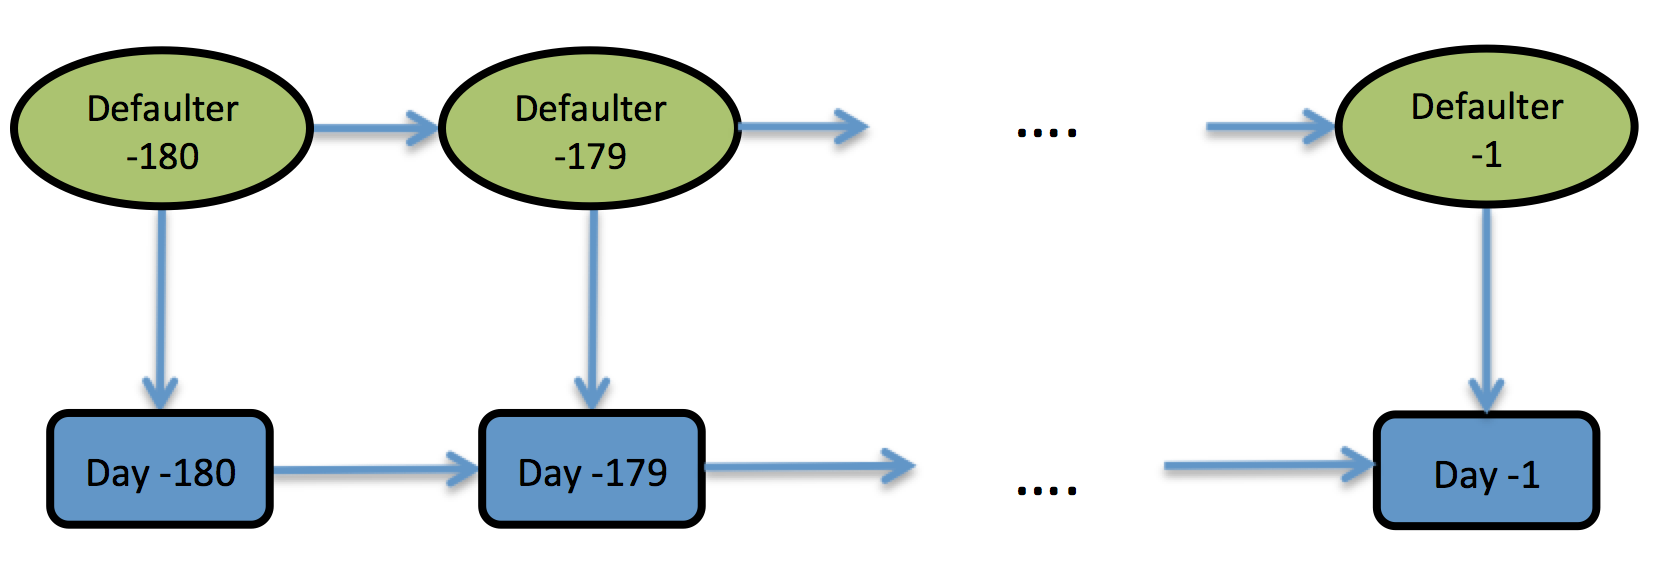
\includegraphics[scale=0.45]{./figures/CajaMarModel1}
\caption{Global structure of the dynamic model. Each blue box represents a set of variables measures during the same day.
The variables within a box can be connected as well as variables between two consecutive days representing the same attribute. For the ease of presentation past paying behaviour and sociodemographic variables are omitted from now on.}
\label{fig:global_temp}
\end{center}
\end{figure}

\begin{figure}[htbp]
\begin{center}
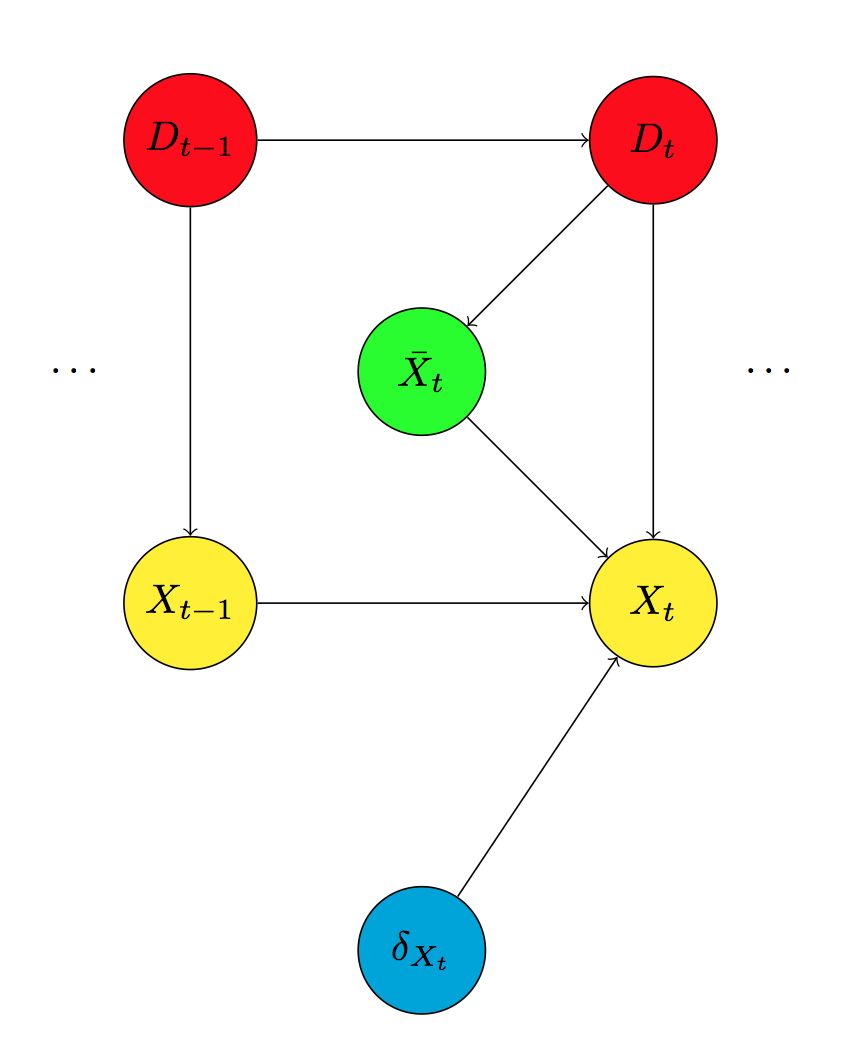
\includegraphics[scale=0.45]{./figures/CajaMarModel2}
\caption{Basic component of the structure of the dynamic model.}
\label{fig:component}
\end{center}
\end{figure}

\begin{figure}[htbp]
  \centering
   \begin{tabular}{cc}    
       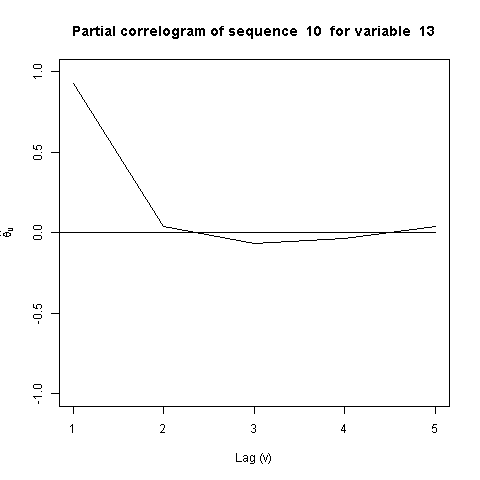
\includegraphics[width=70mm]{figures/CajamarPartialCorrelogram} &
        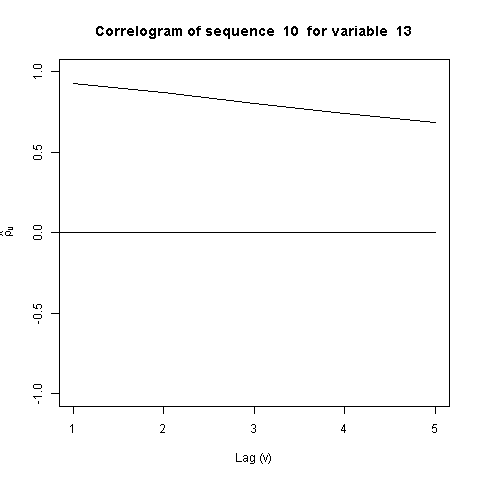
\includegraphics[width=70mm]{figures/CajamarCorrelogram}
    \end{tabular}
     \caption{\label{fig:CajamarCorrelogramsAndPartial} Partial correlogram and correlogram for a variable. A first order Markov assumption seems reasonable to capture dependences over time.}
\end{figure}


Finally, an indicator variable $\delta_{X_t}$ may be included if the variable contains 0 values many times. This is the case for every day payments made by credit card or the historical monthly outstanding amount on the account for instance, whose value can be equal to zero for a large number of days for most customers. For example, Figure \ref{fig:CajamarZeroes} (left) displays the histogram of a variable including all values, and Figure \ref{fig:CajamarZeroes} (right) when the zero values are not considered. Note that the fitted density when the zeroes are discarded are extremely more representative that including zeroes. This result undoubtedly justifies the use of this indicator variable.

\begin{figure}[h]
  \centering
    \begin{tabular}{cc}    
       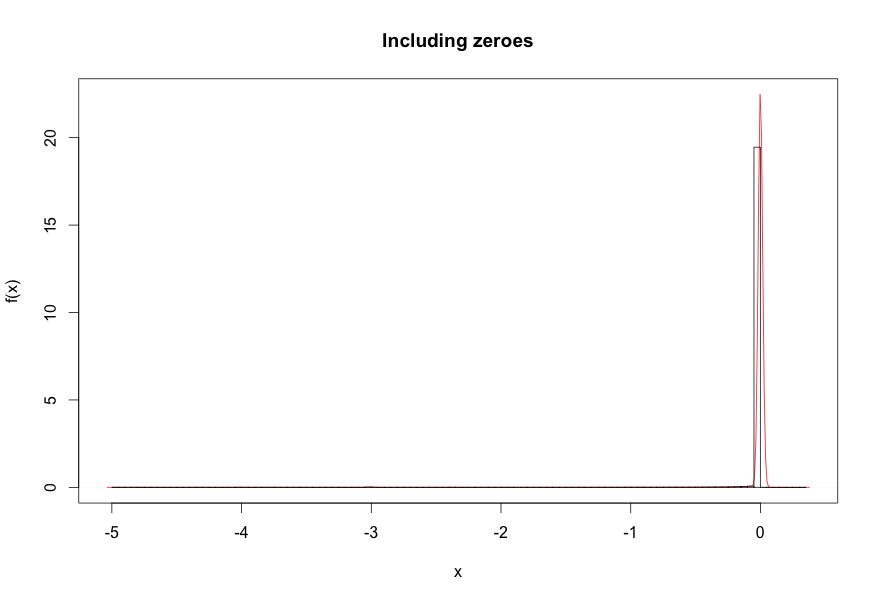
\includegraphics[width=70mm]{figures/with_zeroes}&
       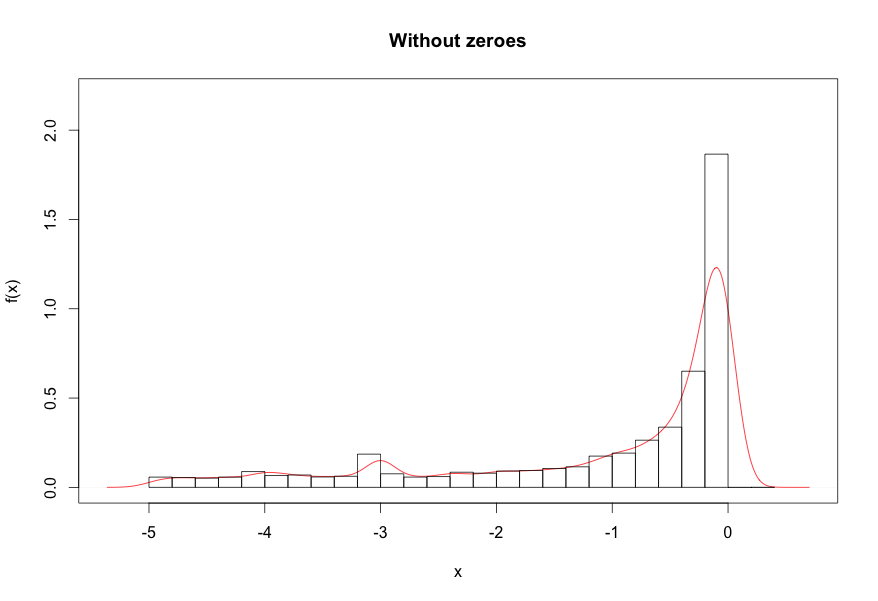
\includegraphics[width=70mm]{figures/without_zeroes}
    \end{tabular}
    \caption{\label{fig:CajamarZeroes}Data histograms and fitted densities for the same variable including zeroes (left) and discarding them (right).}
\end{figure}

On the other hand, there exist some variables that, even though some dependences over time would expected, they do not display any type of dynamic behaviour. This is for instance the case for variables whose correllograms in Figure \ref{fig:cajamarCorr} show values very close to zero for all lags. These variables are hence not linked through consecutive time steps in the dynamic model and are represented by $Y_{t+1}$ in Figure \ref{fig:component} together with sociodemographic variables.

\begin{figure}[h]
  \centering
    \begin{tabular}{cc}
    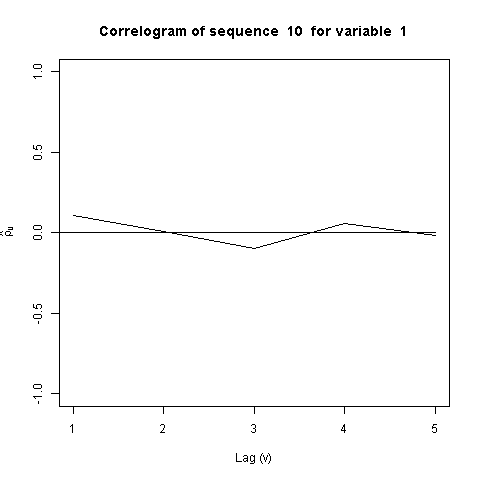
\includegraphics[width=70mm]{figures/CajaMarcrl1}&
     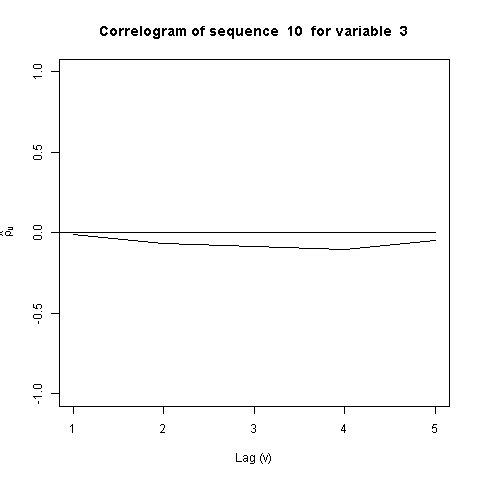
\includegraphics[width=70mm]{figures/CajaMarcrl3}\\
  \end{tabular}
    \caption{\label{fig:cajamarCorr}Correllogram for two variables. No temporal dynamic is shown.}
\end{figure}

In summary, the process of building this dynamic model from the original relational database 
is exactly the same as for the static model.

%%%%%%%%%%%%%%%%%%%%%%%%%%%%%%%%%%%%
\subsubsection{Low risk profile extraction}
%%%%%%%%%%%%%%%%%%%%%%%%%%%%%%%%%%%%
\subsubsection*{Introduction of the problem}

The marketing department at Cajamar periodically launches marketing campaigns for the recruitment of new products by customers (i.e. a new credit card, an insurance, ...). The success of these campaigns depends greatly on the client group to which the campaign has finally targeted. It is also crucial to reduce as much as possible unnecessary expenses focused on non-potential customers. 

For this purpose, the marketing group proceeds as follows. First, they filter the customers using their own marketing models and also, in collaboration with the risk department, select a subset of predictors considered relevant to be part of the final profile (mainly sociodemographic variables). For example, the age of a client is a relevant predictor when designing campaigns to attract customers for a death insurance. 

After obtaining this first group of customers for the campaign and determining the set of relevant attributes, the model proposed in Section~\ref{SubSection:Predicting} will be used to identify the profiles of the less risky clients using the most probable explanations (MPE) method (\emph{defaulter} variable is evidenced to \emph{No}) . Thus, the target customers previously filtered can be now grouped and ranked using these profiles.


\subsubsection*{Static model}
\label{sec:StaticModel}

As pointed out before, mainly sociodemographic variables will determine the customer profiles used in the campaigns. These variables are mostly static as they do not change frequently over time (e.g. marital status, sex, type of job, ...). However, to enhance the analysis a number of  variables changing over time will be included, although due to complexity reasons we should reduce this number as much as possible to make the profile extraction problem feasible.
The structure for the static model proposed in the profile extraction is the same as for predicting the risk of defaulting (see Fig.~\ref{fig:CajaMarModel0}) but with a considerable reduction in the number of predictors used. 

%\begin{figure}[h]
%\centering
%%\begin{tikzpicture}[->,>=stealth,shorten >=1pt,auto,node distance=2cm,semithick,
%%        azul/.style={fill=cyan,rectangle,draw},
%%        verde/.style={fill=green,ellipse,draw}]
%%        \node[verde] (default) {Default};
%%        \node[azul] (predictors) [below of=default] {Predictors};
%%        \draw (default) to (predictors);
%%\end{tikzpicture}
%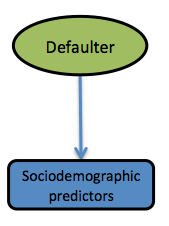
\includegraphics[width=35mm]{figures/CajamarProfileExtractionBN}
%\caption{Static Bayesian network for the profile extraction. The predicting variables can be connected to conform an augmented Bayesian classifier.}
%\label{fig:StaticBNProfile}
%\end{figure}



%---------------------------------------------------------------------------------------------

%
%Note that past information about the variables are not considered for this problem as it was for predicting the probability of defaulting in Section~\ref{SubSection:Predicting}. In this model the latest information about the variables are considered instead.

For the profile extraction, the model not necessarily must have a classifier structure but it can have a general structure instead. However, what is desirable is to avoid using a NB structure for this task. The reason is that once the \emph{defaulter} variable is evidenced to \emph{No}, the predictors become independent and the analysis would be poorer (MPE in this case would correspond to the maximum probability value for each variable individually).



\subsubsection*{Dynamic model}

As mentioned in Section~\ref{sec:StaticModel} the profile extraction problem mainly uses sociodemographic variables but in practice it might happen that variables related to financial activities or paying behaviour are required to be included in this model.  For instance, it could be of interest to include in a profile the tendency of a variable, i.e., the balance of a customer in the last days. For these reasons we should consider the modelling of a dynamic version for the profile extraction. 

The model for the profile extraction is the same as the one depicted in Figure~\ref{fig:component} but, as for the static approach, with a considerable reduction in the number of predictors. 

%\subsubsection*{Model Structure}
%
%From a probabilistic modelling point of view, Caja-Mar faces two different problems [][]: the prediction of the risk of defaulting of a customer in the next two years; and the extraction of profiles of ``desirable'' prospective customers. 
%
%The risk prediction problem has been modelled as supervised dynamic prediction problem.  We are given a data base with a set of variables or predictors (some of them manually built by CajaMar's experts) describing the financial behaviour of the customers and, also, whether the customer is considered as defaulter and non defaulter according to CajaMar standards (i.e. a binary class variable). The dynamic component of the problem needs to be considered because the behaviour of the customers evolves over time (e.g. the account balance is continuously changing from month to another, the level of incomes, etc.)  as well as the labelling as defaulter or non-defaulter customer (e.g. one customer can be creditworthy and, but after some time, be in bankrupt for becoming unemployed). More specifically, the proposed model is expected to answer the following question: which is the probability that this customer will  default in some of his/her loans in two years? And this prediction has to be made only using the customer's behavior in the last 180 days \footnote{This limit is imposed by the Bank of Spain.}.
%
%The graphical structure of the dynamic probabilistic graphical model devised for this problem is given in Figure \ref{Figure:CajaMarModel1}.  The yellow square boxes ``Day -180'', ..., ``Day-1'' represents the temporal evolution of the predictor variables. The model only refers to 180 days because this is the imposed limit of days when making predictions. Similarly, the class variable ``default'' is assumed to evolve over time but with the relevant different that the default class sequence refers to a point in the time \textbf{two years later} than  the point in the time the daily predictor variables. 

\subsubsection{Discussion and future models}




% !TEX root = D2.1_AMIDSTModellingFramework.tex
\subsection{Verdande Models}
\label{Section:VerdandeModels}


%\subsubsection{Introduction}

As has been pointed out in Delivrable D1.2, three main tasks have to be addressed for Verdande Technology use case:

\begin{enumerate}

\item \textbf{Automatic detection of drill string vibrations and abnormal torque states} which aims to better diagnose the shape of the wellbore and the state of the equipment, make better decisions on how to manage the well, and thereby reduce the non-productive time. To this end, a probabilistic graphical model for erratic torque monitoring and detection will be used.


\item \textbf{Semi-automatic labelling}: Given unlabelled data streams collected over time from typical drilling conditions, semi-automatic labelleing aims to compute a normality score for each considered drilling situation, then label it as either "normal" or "abnormal". As previous task, a probabilistic graphical model will be used, taking into account of the temporal dynamics of the drilling process and continuously adapting to changes in the incoming streaming data. Semi-automatic labelling allows to reduce the non-productive time and improve as well the data quality.

\item \textbf{Automatic formation detection}: which aims to predict in real time the formation tops from the MWD (measurements while drilling) data using a probabilistic graphical model. Once again, this should be performed taking into account of the temporal dynamics of the drilling process and continuously adapting to changes in the incoming streaming data. The automatic formation detection is vital for dealing with several issues such as hole instability and vibrations, and also important for reducing the costs and the overall non-productive time.
\end{enumerate}

For all tasks, the model must deal with both continuous and discrete observed random variables. Moreover, the oil-well data to be used presents the following characteristics: 

\begin{itemize}

\item It has a dynamic structure consisting of \emph{long-term} patches (ranging from a couple of hundred observations and into the thousands). Inside a patch, the data is typically fairly \emph{stable} and with low noise, even if this is not always the case. Between the patches the data can vary a lot. A \emph{patch of data} typically corresponds to the implementation of one activity (like drilling, connection tripping in/out, etc.). Consequently, the models would be better designed locally inside each single patch.

\item Inside one activity, many of the attributes can be strongly correlated. The observed correlation between variables $X$ and $Y$ can either be instantaneous (i.e., corr($X_t, Y_t$) significant), or delayed to some extent (i.e., exposed through the correlation corr($X_t, Y_{t+k}$) for some fixed $k$).

\item Physical models can be used to understand why these correlations are there, but not to quantify them. In addition, sometimes the strength, and even the sign, of the correlation may change from well to well.

\end{itemize}



\subsubsection{Detection of drill string vibrations and abnormal torque states}\label{SubSection:DetectionTorque}

{\bf Sigve: Add some oil-lingo to explain why this is a problem worth looking at}




Two time-windows of torque-readings are given in Figure \ref{Figure:VTTorqueValues}; the uppermost plot traces the torque over a period of 25.000 observations, the other is zoomed in to cover only 500 observations. It is evident that the torque varies over time, and often drops to zero (in particular when the drill-bit is not rotating). Furthermore, we can see from the zoomed-in trace that the variance changes over time; this time-window commences with rapidly varying torque, before the variation is reduced. The goal is to extract passages where high variance in the observed torque cannot be explained by other drilling parameters. 
We will begin the following discussion by considering how to model the torque as a random variable developing over time, without thinking about vibration and the variable's relationship to other drilling parameters.   
Thereafter, a full model will be proposed.

\begin{figure}
\begin{center}
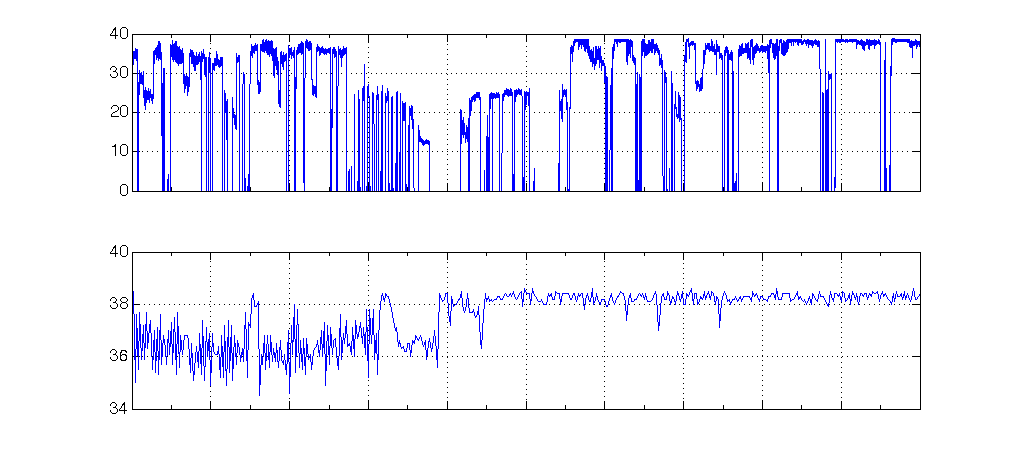
\includegraphics[scale=0.3]{./figures/VT_TRQ_values} 
\caption{\label{Figure:VTTorqueValues}  Measurements of TRQ.}
\end{center}
\end{figure}


The autocorrelation and partial autocorrelation of the torque can be seen in Figure \ref{Figure:VTTorqueAutoCorr}. It is clear that a significant autocorrelation exists, also at high lags. The figure goes up to $k=20$, where the correlation is still above .6; note that the only data from drilling (i.e., where the torque is positive and ``moving naturally'') have been included. A model capturing the time dynamic is therefore essential. Furthermore, the partial autocorrelation shows very significant contributions at lags 1 and 2, and also significant effects at lags 5--10.  

\begin{figure}
\begin{center}
\begin{tabular}{c@{}c}
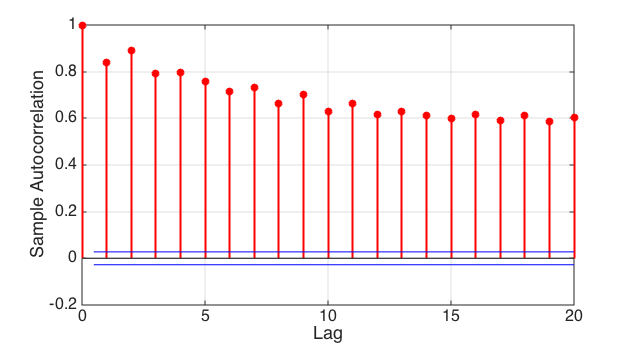
\includegraphics[scale=0.3]{./figures/VT_autoCorr_TRQ} &
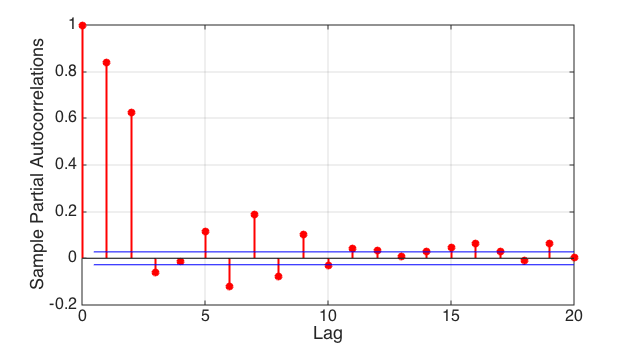
\includegraphics[scale=0.3]{./figures/VT_partialAutoCorr_TRQ}  \\
Autocorrelation & Partial autocorrelation
\end{tabular}
\caption{\label{Figure:VTTorqueAutoCorr}  Whatever.}
\end{center}
\end{figure}


To capture the dynamics of this variable, we propose a Kalman filter model, with a ``sufficiently rich'' latent variable space (that is, more than a single one-dimensional latent variable may be required to capture the partial autocorrelations in the data).  {\bf NEED TO SHOW FIGURE WITH THE KALMAN FILTER?}



Next, we consider how to model a torque sequence that also includes  abnormal torque measurements (those that are corrupted by vibrations). 
Our working assumption is that an abnormal torque signal is the result of a string vibration with higher frequency than the sampling frequency of the data. Thus, it will be observed as a white-noise signal superimposed on top of the ``true'' underlying torque signal. An abnormal torque regime will typically last for some unknown time significantly longer than one time step, thus we must create a model with the ability to choose a state that fits the observations best (normal or abnormal), and with a tendency to remain in a chosen state over time. This can be obtained by a switching Kalman Filter, where the switching variable (connected over time) is used to show which state one is in at a given time (normal or abnormal) and the transition model for the variable is used to capture the state remaining for some time. 

{\bf SHOW dBN?}

Preliminary results using this class of models, but without learning the parameters properly, and relying on an inference scheme that does not scale to the data-sizes we have available in the AMIDST project are shown in Figure \ref{Figure:VTEraticTorqueMarked}. The same subset of data used in Figure \ref{Figure:VTTorqueValues} is once again used, and the positions the system detects as having ``abnormal torque'' is highlighted along the $x$-axis. These annotations correlate well with what can be obtained by simple inspection of the time series with the human eye. Still, some undesired observations remain. For instance, the two  areas with small dips in the observed torque towards the end of the sequence can be explained by specific drilling activities going on ({\bf Sigve: I think this was a connection because (as far as I remember) ROP is zero here. Not really sure,though. Is it correct?}), and should not be marked as outliers. To understand that these observations are not abnormal, the context of the torque observation must be includes, which is what we turn to next.

\begin{figure}
\begin{center}
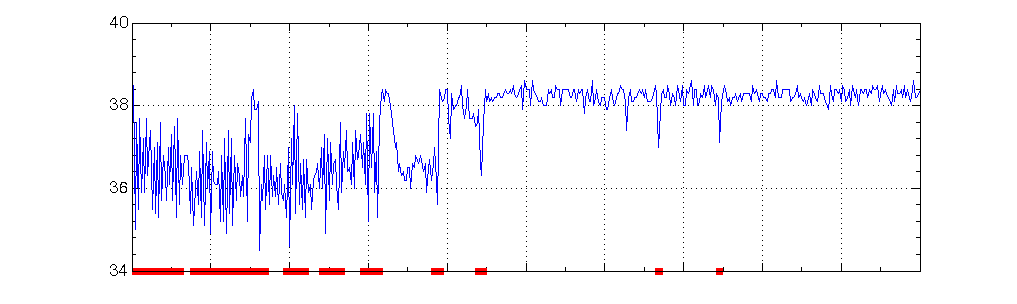
\includegraphics[scale=0.3]{./figures/VT_ErraticTRQ_marked} 
\caption{\label{Figure:VTEraticTorqueMarked}  Whatever.}
\end{center}
\end{figure}



{\bf Sigve: Say why ROP is the most relevant ``driver''-variable.}





To examine the relationship between ROP and TRQ further, we plot the joint density of (ROP$_t$, TRQ$_t$) and the sample correlation between ROP$_t$ and TRQ$_{t+k}$ in Figure \ref{Figure:VTTorqueRateOfPenetration}. We notice that even if a strong correlation is not apparent in the density plot, if can be seen as significant form the correlation plot, and should therefore be included in the model. We capture this through an \textit{input-output Kalman filter}, where the ``input'' at time $t$ is the rate of penetration at that point in time, the ``output'' of the Kalman filter is the (observed) torque readings, and where we have to sets of latent variables: $i)$ a discrete switching variable, which is used to signify which torque regime we are currently in, and $ii)$ a latent vector of continuous variables used to capture and model the natural behavior of the torque sequence over time. During inference, the posterior probability of the discrete latent variable at time $t$ can be used to detect whether or not the system experiences abnormal torque (that is not explained by the observed rate of penetration) over time. 

Further extensions to the model, where also other predictive variables are taken into account, will be considered at a later stage. The general model structure will, however, not be changed.


\begin{figure}
\begin{center}
\begin{tabular}{c@{}c}
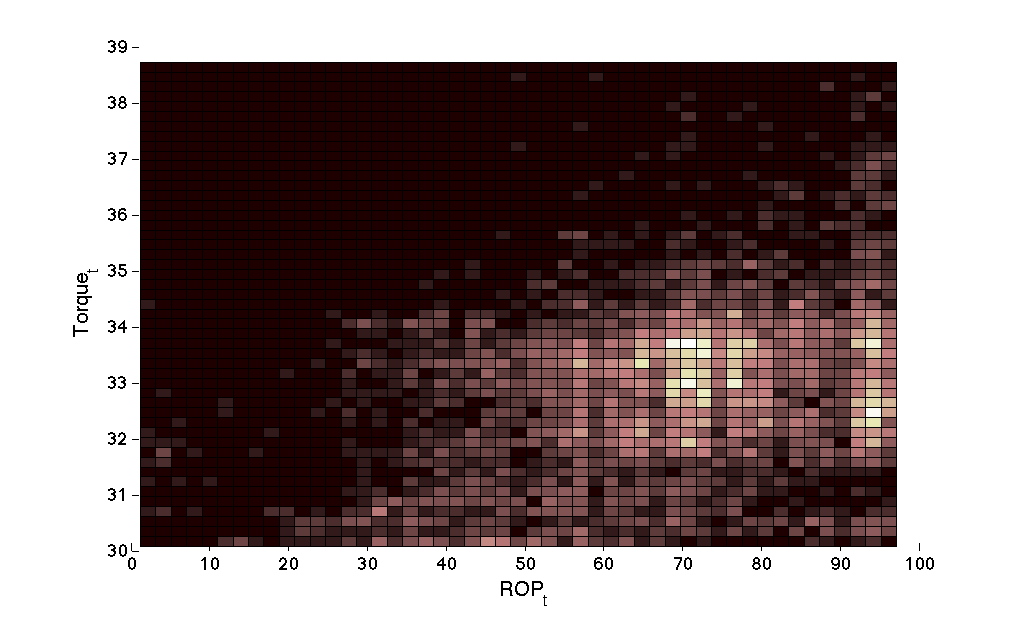
\includegraphics[scale=0.2]{./figures/VT_TRQ_ROP_density} &

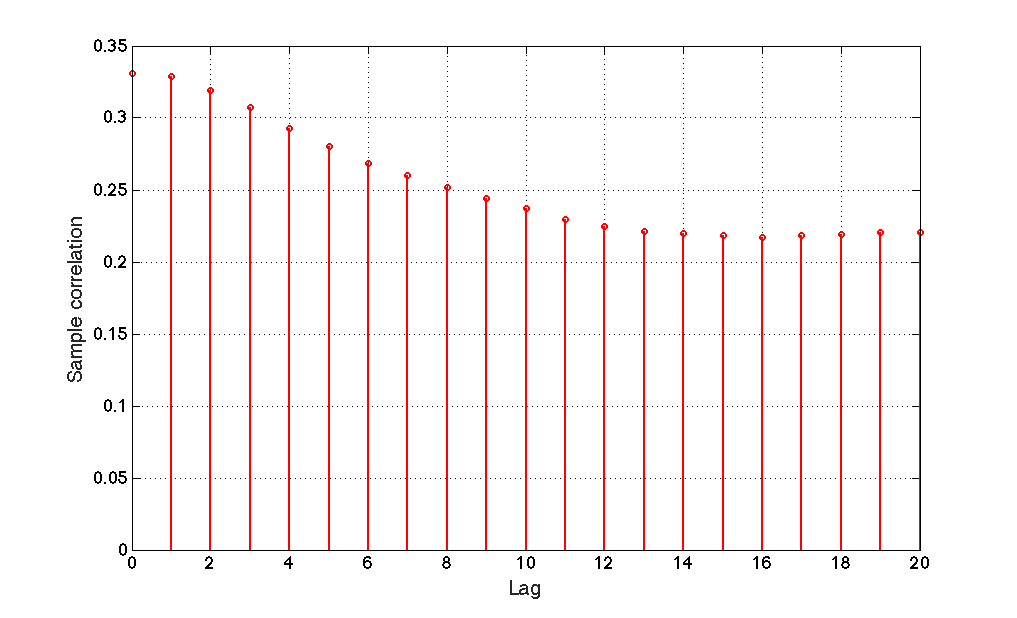
\includegraphics[scale=0.2]{./figures/VT_crossCorrTRQvsROP}  \\

\end{tabular}
\caption{\label{Figure:VTTorqueRateOfPenetration}  Whatever.}
\end{center}
\end{figure}






\subsubsection{Semi-automatic labelling}\label{SubSection:SemiAutomaticLabelling}

The main contribution from DrillEdge during operation is that it enables the driller to see in real time if the current situation is ``similar'' to previous situations that lead to undesired circumstances. 
If this is the case, remedial actions can be found to avoid undesired events. 
At the core of the analysis are historical examples of noteworthy episodes, ranging from clearly undesired events, for instance getting stuck, to more subtle indications of evolving problems, such as abnormal readings of hook-load. 
Verdande Technology has already extensive datasets (made available to the project from its beginning), where such episodes are identified. 
However, the definitions of the episodes are not always crisp, and domain experts can at times disagree about what is happening at a certain time. 
This can potentially lead to inconsistencies in the dataset, complicating both the automatic learning of models as well as the comparison with previous situations. 
Additionally, it can confuse the driller to be presented with information that he/she does not relate to or agree with.

Manually labelling new data sequences, or adapting the existing labelling to new definitions, can be a very time-consuming activity, and Verdande Technology therefore want to start looking into techniques for semi-automatic labelling.
This process is initiated by the system being fed with unlabelled data streams from typical drilling conditions. The system should adapt to this data, and recognise what is ``normal'', both with respect to auto-correlations of each variable over time, as well as the intricate relationships between variables. Simultaneously, sub-sequences that do not fit well with the normal data should be marked as ``abnormal''.
The abnormal sub-sequences can thereafter be examined more closely by drilling experts. It is desired that the process should be able to take back information from this examination, and update the reasoning if the sequences marked as abnormal were not correctly labelled. The benefit of the automatic tagging is that more time can be spent on scrutinizing the ``interesting'' parts of the drilling logs, and less time on the ``normal'' parts. 
This implies the potential for further reduction in non-productive time. Specifically, the goal is to provide a ``normality'' score for historical logs to facilitate semi-automatic detection of abnormal situations. The calculations should be efficient enough to run in real time if so desired.

Drilling is performed in phases, where different activities are conducted in sequence. For instance, one can only drill the well (increase the length of the well-bore) after having transported the drill-bit to the bottom of the well (that is, performed a ``tripping-in'' activity). Similarly, a long drilling sequence is split up into smaller sequences, where each subsequence is initiated by a ``connection'' activity, where the length of the drill-string is increased.
The division of the drilling log into subsequences containing only a single activity is done automatically by Verdande Technology's Drill Edge system. 
Therefore, the AMIDST system will be fed sequences where a single activity is conducted. 
The behaviour during each of these sequences  is fairly consistent if the process runs smoothly, and the relationships between variables can be established (e.g., the amount of mud transported into the drill-string will, after stabilization, be strongly indicative of the amount of mud coming out after circulating through the well string). 

Some of the variables in the data set are used to monitor quantities that are set externally by the drilling crew (examples include ``weight-on-bit'', ``rotations-per-minute'' and ``mud-flow-in''). Other variables, like ``torque'', ``rate-of-penetration'' and ``mud-flow-out'' can be understood as  (possibly delayed) responses to the input from the geology. The cause $\rightarrow$ response relationships are mostly unknown, but some qualitative understanding exists. {\bf Sigve: Is that correct? Can you give an example?}

The measurements are continuous, but not necessarily Gaussian. We therefore propose to use an input-output Kalman filter with Gaussian mixtures at the leaves to model a data stream from a single subsequence. The normality-index for an observation ${\bm e}_t$ at time $t$ given the observations up until $t$, ${\bm e}_{1:t-1}$ will be calculated as the log conditional likelihood,  $\ell_t := \log f\left({\bm e}_t|{\bm e}_{1:t-1}\right)$. By monitoring  $\ell_t$ over time, significant departures from its ``typical behaviour'' will be noted, and marked as potential irregularities.

{\bf Do we need to show the input-output-KF? What about the structure of the analysis for the $\ell_t$-terms?}


\subsubsection{Automatic formation detection}\label{SubSection:DetectionFormation}


In many drilling operations, a precise recognition of a formation change can be vital for cost savings. 
For instance, it is important to cement the casing in the correct formation, to manage the formation pressures as well as correctly identifying the top and the bottom of an oil reservoir. 
Additionally, accurate knowledge of the formation allows the drilling crew to optimise drilling parameters and better diagnose the condition of the bit. 
Knowing the formation is also an important input in how to deal with symptoms such as improper hole-cleaning, hole-instability and vibration issues. 
A proper formation detection is therefore an important piece in the puzzle for reducing the overall non-productive time.

Before the well is drilled, a chart with the expected formation tops is available from the well plan. The chart is based on seismic data and drilling data from neighbouring wells and contains the best guesses on which depths the various formation tops are located. Since it is uncertain where the formation tops are, an uncertainty interval is associated with every formation top. This is called the lithology chart.

In practice, the prediction of the formation tops is refined by a human, who interprets  {\em measurement while drilling} (MWD) data, and aligns this with the lithology chart as the well is being drilled. 
The MWD data measures petrophysical properties of the rock such as gamma radiation, sonic speed and electrical resistivity. 
Often, shifts in these graphs happen when the formation is changing. We will therefore formulate the formation detection problem as change-point detection in a multivariate data stream. 
Indications of change-points (shifts) are to be compared with the prior belief to specifically locate the changes. 

The prior information, giving the expected locations (depths, in meters) of formation change, together with a degree of certainty (in terms of a standard deviation) is the point of departure for this model. Let us assume that there the drilling crew a priori expects  to see $N$ changes in formation. 
This information may be erroneous, as any number of additional formation-changes (that were not expected in advance) may also occur in the ground, e.g., if a one a priori expected formation of sandstone for 100 meters, later realizing that this sediment was split into two by a small layer of shale {\bf SIGVE: Is this meaningful? I'm just inventing a story here, and do not know what shales is :-)}.
The observation data is encoded wrt.\ \textit{time}, and but will be used with an encoding wrt.\ \textit{depth} in this application to have it aligned with the prior information at hand. The data may not necessarily be equally spaced (e.g., two neighbouring observations may be separated by 3mm, while the two next are separated by only 2mm). 
 

Again, we think in terms of an input-output Kalman-filter, but this time the latent variables will have a predefined structure:
\begin{itemize}

\item The input variable at time $t$, Depth$_t$, is the dept of the bit at that time.

\item The next chain of variables are \textit{counting-variables}, denoted FormationNo$_t$. The variable has two parents: Depth$_t$ and FormationNo$_{t-1}$. 
The probability that the counting variable is incremented at time $t$ conditioned on the parent configuration is calculated by combining information from the prior information with the parents' configuration. Logistic or probit functions can  be imagined, but must be compared to the actual domain knowledge to give a feasible representation.

\item Shift$_t$  generates a  chain of variables used for determining when   a formation-change actually occurs. It has two parents, namely  FormationNo$_{t-1}$ and  FormationNo$_t$. 
The variable is discrete, and has three states: ``No -- As accounted for in the prior'', ``No -- But expected in prior'', ``Yes -- As accounted for in the prior'', and ``Yes -- But not expected in prior''. 
To this end, FormationNo$_t$ only changes when expected by the prior information, while Shift$_t$ can use the data to refine these assessments. If $\mbox{FormationNo}_{t}= \mbox{FormationNo}_{t-1}$, Shift$_t$ is in the state 
 ``No -- As accounted for in the prior'' with probability $1-\epsilon$ and in state ``Yes -- But not expected in prior'' with probability $\epsilon$. If $\mbox{FormationNo}_{ t}=\mbox{FormationNo}_{t-1}+1$, Shift$_t$ takes the state 
``Yes -- As accounted for in the prior'' with probability $1-\delta$ and ``No -- But expected in prior'' with probability $\delta$. $\epsilon$ and $\delta$ are parameters to be determined through expert knowledge or learned from data.

\item Finally, the observed variables at time $t$ only have  Switch$_t$ as parent. We will not use the actual observed sensor reading as the observed variable (``output-variable'' in the input-output Kalman-filter). Rather, the differences are used, e.g., GammaRay$_t$ - GammaRay$_{t-1}$ will be used to represent the gamma ray measurement at time $t$. These variables will, given that Switch$_t$ is in the ``No''-states, vary around zero. The variable will be significantly different from zero if the parent is in any of the ``Yes''-states.
\end{itemize}

{\bf Get a data plot of the GammaRay and its diff to show how the diff run around zero except when we have formation changes. Would not only show the idea of the model, but also indicate that the assumptions make sense. And show that data is available from day 1 and all that. SIGVE: You supply me with the data?}

At the time of inference, we condition on the total number of switches, and calculate (using forward-backward) the posterior distribution of the locations. Similarly, we will also calculate the most probable explanation, that is, the most probable configuration of switches given the total number of events.


\subsubsection{Discussion and future models}


Not sure what to put here?!




\section{AMIDST Model Class}

\subsection{Introduction  and Notation}

One of the main goals of this project was the definition of a general model class which the following features: (i) it has to be applicable to the three use-cases; (ii) it should be general enough to apply to other future similar use-cases;  (iii) and it should contain certain structure that can be exploited to make this model class valid for scalable inference and learning in massive data streams. 

With these three aims in mind,  we started the definition of the general model class by finding commonalities between the different models presented in Section \ref{Section:PreliminaryModels}.  With this aim, we  introduce some new ``graphical'' notation to ease this process. This new graphical notation is based on the use of subnetworks modules, i.e. some part of the dynamic Bayesian network with some common features such as all the nodes are continuous and observed.  We represent these subnetworks modules by square boxes, in opposite to circle or ellipsed nodes used to represents single variables in a graph. Following a similar notation we used for nodes (see Figure \ref{Figure:PreliminariesNotation}), square boxes rounded by dashed lines refers to a subnetwork which is not observable (i.e. composed by hidden variables); square boxes rounded by continuous lines refers to a subnetwork where the nodes are observed; when the square box is coloured, it means that all the nodes of the subnetwork are discrete (green color) or continuous (blue color). Square boxes can also be nested to represent smaller subcomponents inside a bigger subcomponent. In Figure \ref{Figure:ModelClass:Notation} we give a visual description of this notation. 

\begin{figure}
\begin{center}
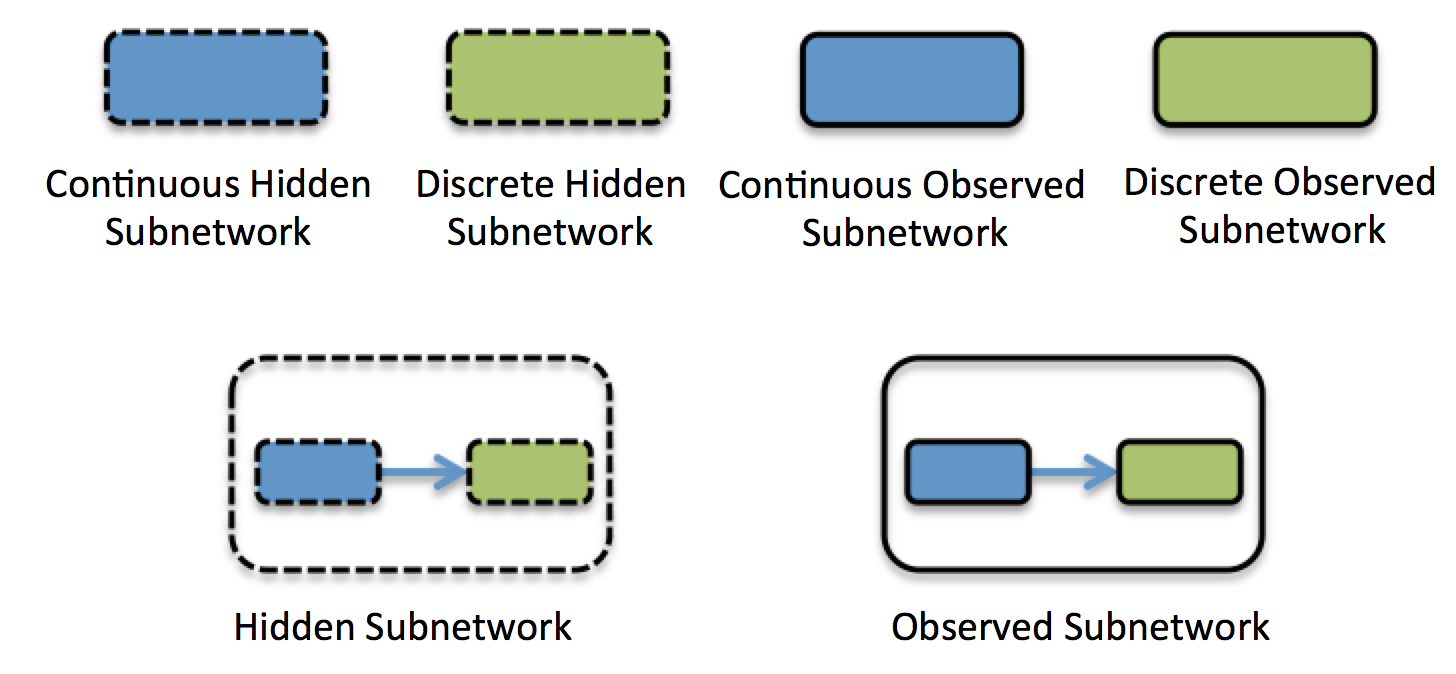
\includegraphics[scale=0.4]{./figures/ModelClass0}
\caption{\label{Figure:ModelClass:Notation} Graphical Notation}
\end{center}
\end{figure}

We present now the models of the three use-cases but using this previously introduced notation. This reinterpretation of the models presented in Section \ref{Section:PreliminaryModels} using these high-level descriptors is made in order to identify the commonalities between all the presented models. 

\subsubsection*{Daimler Model Class}

Daimler's model were visually described in Figures \ref{Figure:daimlerLEdynGeneric}  and \ref{Figure:daimlerreldyn}. As commented in Section \ref{Section:DaimlerDynamic}, one the main issues of these current models is that they contain discrete children with continuous parents and do not fall in the conditional linear Gaussian family \cite{JensenNielsen2007}. We adopt here the same solution pursed in \cite{kasper2012object} which consists on the discretization of these nodes. In that way, the general structure of Daimler's models would be the one plotted in Figure \ref{Figure:DaimlerModelClass}, where do not have any more discrete children with continuous parents which allows for a standard parametrization \cite{JensenNielsen2007}. 

\begin{figure}
\begin{center}
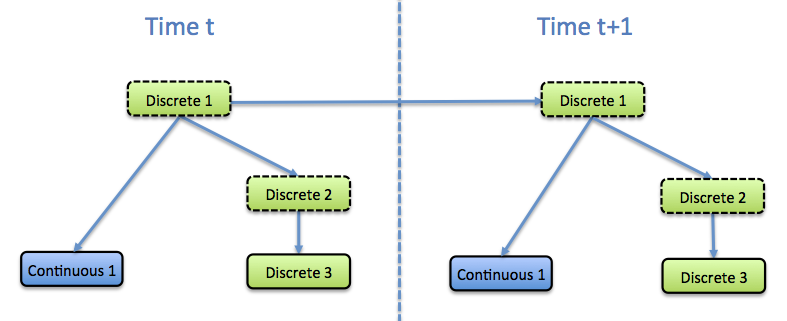
\includegraphics[scale=0.4]{./figures/DaimlerModelClass}
\caption{\label{Figure:DaimlerModelClass} Daimler Model Class}
\end{center}
\end{figure}

This general model is structured as a two-time slices dynamic Bayesian network \cite{JensenNielsen2007}. The static model which is repeated through the time is composed by three elements: a set of hidden discrete nodes on top; and two observed sub-networks, one continuous and one discrete, which directly depends of the hidden sub-network. This dynamic BN is only temporally connected through the hidden sub-network.  In consequence, the future and past time slices of our dynamic BN are conditionally independent given the hidden sub-network corresponding to the present time. Additionally, inside a time slice, the observed continuous and discrete sub-networks are also conditionally independent given the hidden-subnetwork.

We also have more structure that can be exploited during inference and which is not reflected in this meta-network. Specifically, we have that the hidden and observed sub-networks have a poly-tree structure \cite{JensenNielsen2007}. Then, the static BN as well as the dynamic BN both have poly-tree structure and this can be exploited during inference. 



\subsubsection*{Verdande Model Class}

Verdande's models were visually described in Figures ?, ? and ? for the three application scenerios of the Verdande use-case (see Section \ref{Section:VerdandeModels}).
Figure \ref{Figure:VerdandeModelClass} visually describes the high-level model that subsumes the models
of the three application scenarios. If we keep the subnetworks ``Discrete 2'', ``Continuous 1'' and ``Continuous 2'' we have the switching Kalman filter model of application scenario 1 (see Section ?). If we keep ``Continuous 1'', ``Discrete 3'' and ``Continuous 2'' we obtain the model for application scenario 2 (see Section ?). Finally, the model for application scenario 3 is obtained by keeping ``Discrete 1'', ``Discrete 2'' and ``Continuous 2'' (see Section ?).  

\begin{figure}
\begin{center}
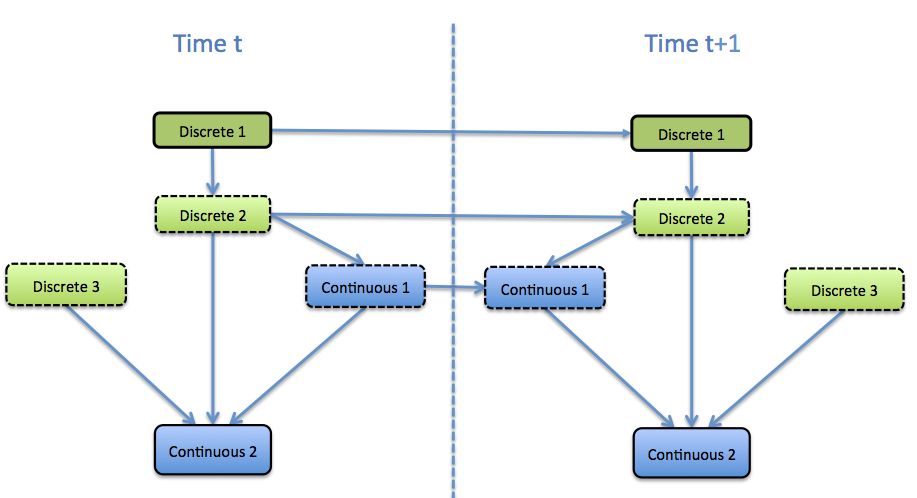
\includegraphics[scale=0.4]{./figures/VerdandeModelClass}
\caption{\label{Figure:VerdandeModelClass} Verdande Model Class}
\end{center}
\end{figure}

Similarly to the Daimler model, the general model is structured as a two-time slices dynamic Bayesian network \cite{JensenNielsen2007}. The static part which is repeated through the time is composed by 5 sub-networks: two observed components, one discrete temporally connected on the top and one continuous at the bottom; and three hidden components in the middle, one hidden discrete and one hidden continuous temporally connected, and one hidden discrete which is not temporally connected whose function is to account for the possible conditional dependencies of the observed continuous variables.  

In opposite to Daimler,  this model does not have a poly-tree structure that can be exploited during inference. 

\subsubsection*{Caja Mar Model Class}

%\begin{figure}
%\begin{center}
%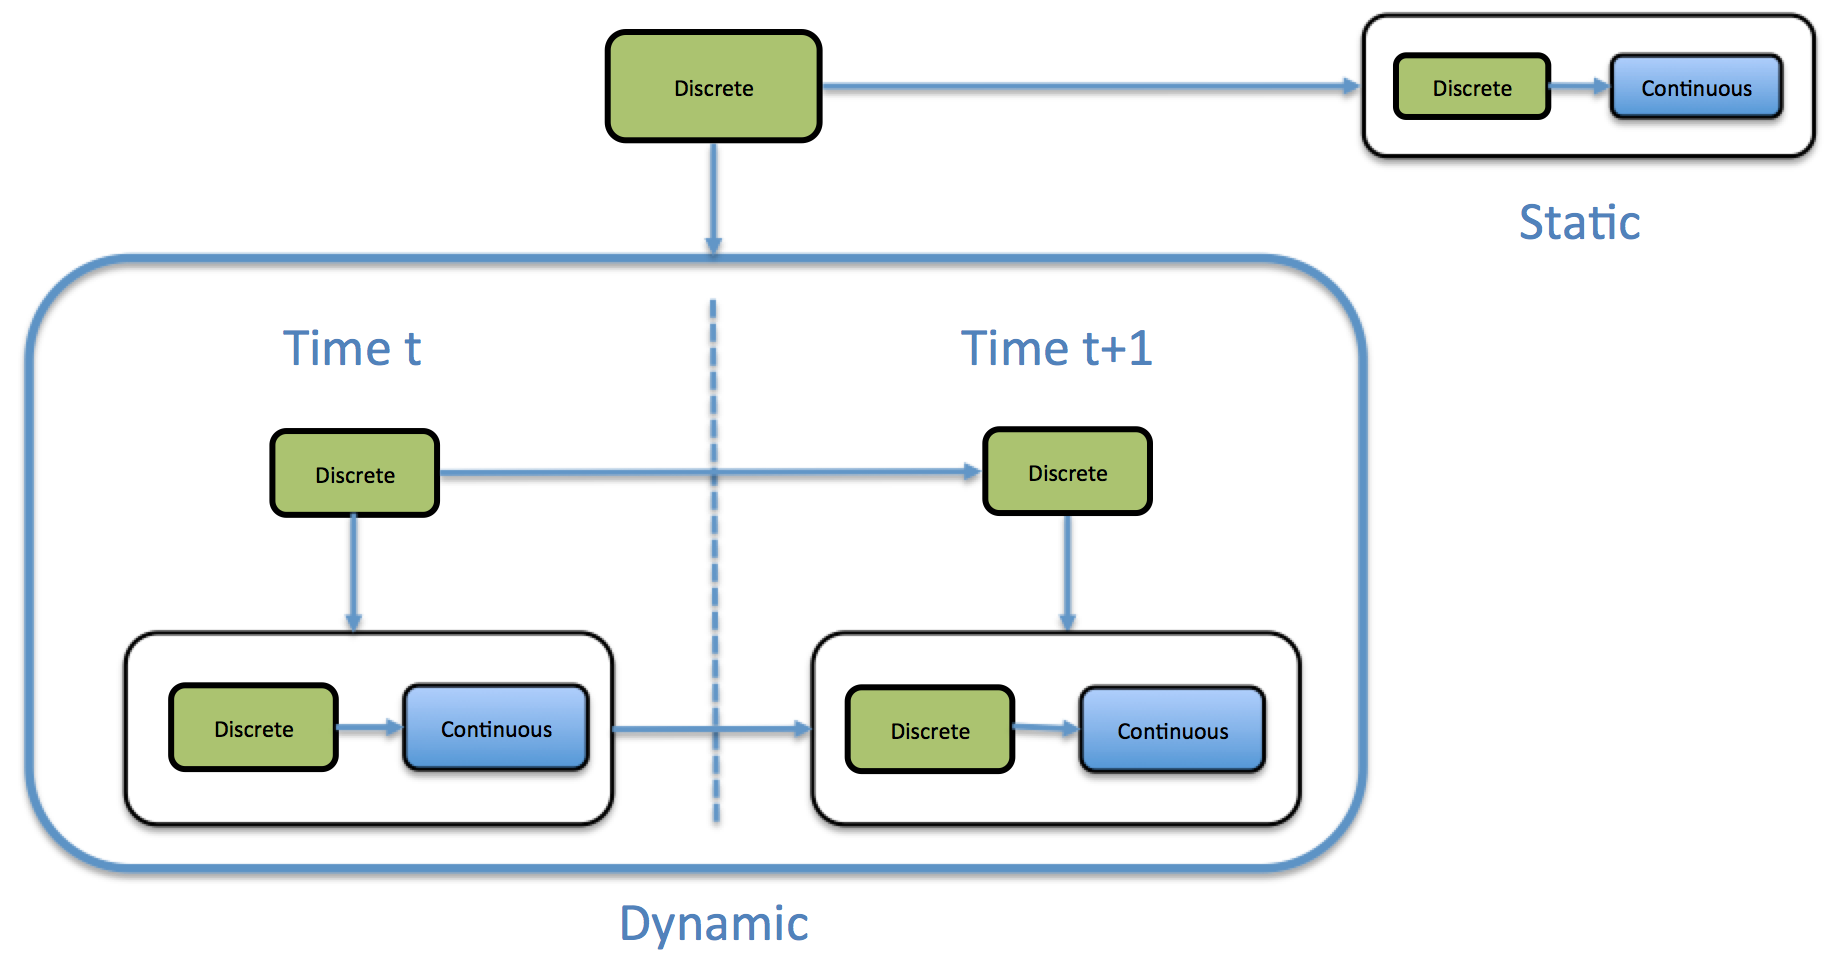
\includegraphics[scale=0.4]{./figures/CajaMarModelClass}
%\caption{\label{Figure:CajaMarModelClass} CajaMar Model Class}
%\end{center}
%\end{figure}



\subsection{AMIDST Model Class}




%\begin{figure}
%\begin{center}
%\caption{\label{Figure:AMIDSTModelClass} CajaMar Model Class}
%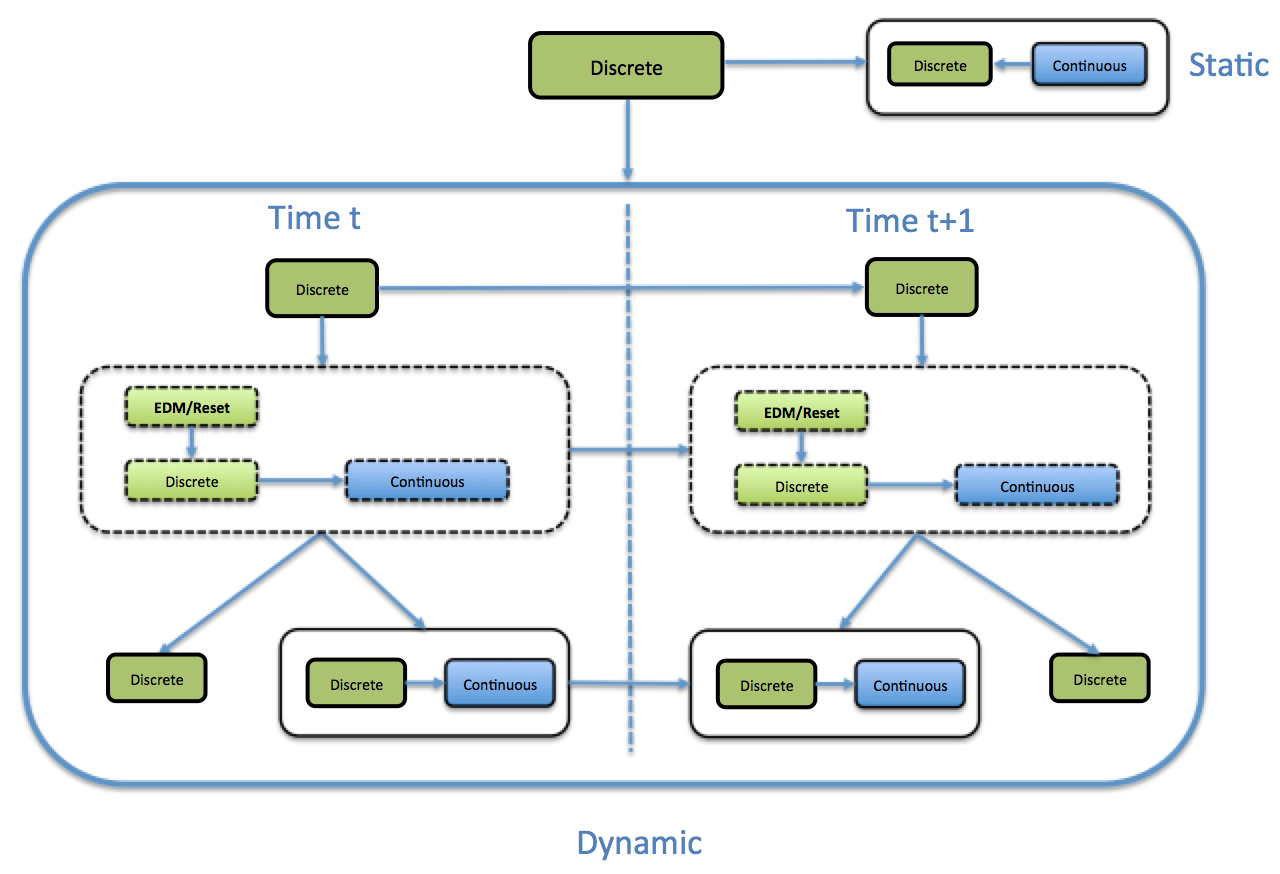
\includegraphics[scale=0.7]{./figures/AMIDSTModelClass}
%\end{center}
%\end{figure}

%\section{Ongoing and future work}

Is is important at this stage to emphasize that this is an ongoing project research and a better understanding of the faced problems and/or future applications might reveal that some elements of this modelling framework need to be refined. As already commented,  we still have to work on inference and learning algorithms that make these models applicable to scenarios dealing with massive data streams. These developments might also has an impact in the current framework, as well as the time and space complexity of the resulting models.

On the other hand, this modelling framework has to provide solutions which achieve levels of performance (e.g. prediction accuracy) which were previously specified in the requirement analysis \cite{Fer14b}.  The analysis of evaluation results obtained by the implemented model, might be another factor that can impact the final specification of this framework. For example, we are now assuming a first-order Markov assumption. One could easily envision the possibility of going to higher order Markov assumptions if the tests reveal that this first-order assumption severely limits the modelling capacities of this framework in some of the application scenarios. 

These refinements of the dynamic model are part of task 2.2. Additionally, we are exploring how to take advantage of certain conditional independences that may arise in the data at a particular time. If appropriately identified, they could be exploited in bounded time horizon models to maintain a fixed efficient time window without loosing expressive power.

All these analysis will be included in deliverable 2.2.



\bibliographystyle{splncs}
\bibliography{biblio}

%\appendix


%\section{Formal framework for requirements elicitation}
%\label{sec:form-fram-requ}
%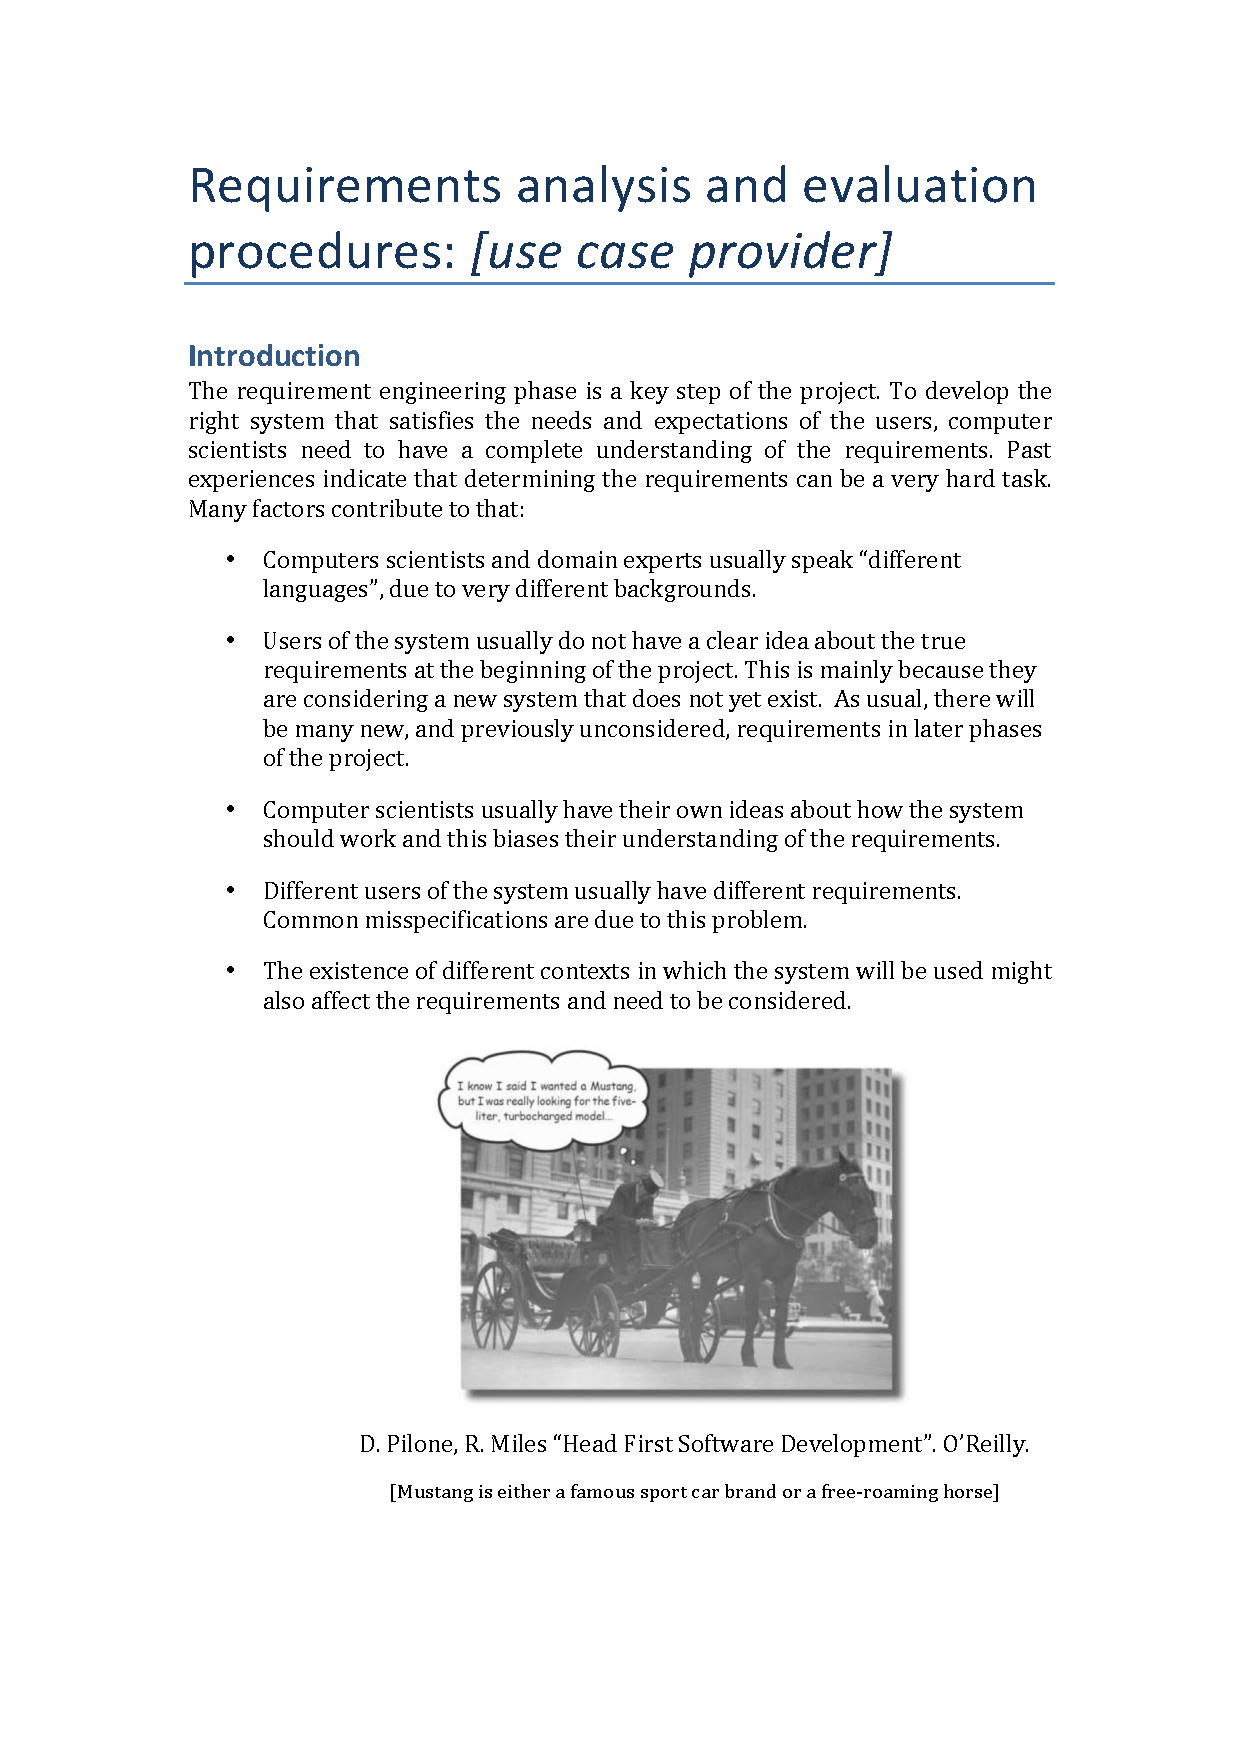
\includepdf[offset=0 1cm,scale=0.85,pages={-},pagecommand={\pagestyle{fancy}}]{appendixA1.pdf}
%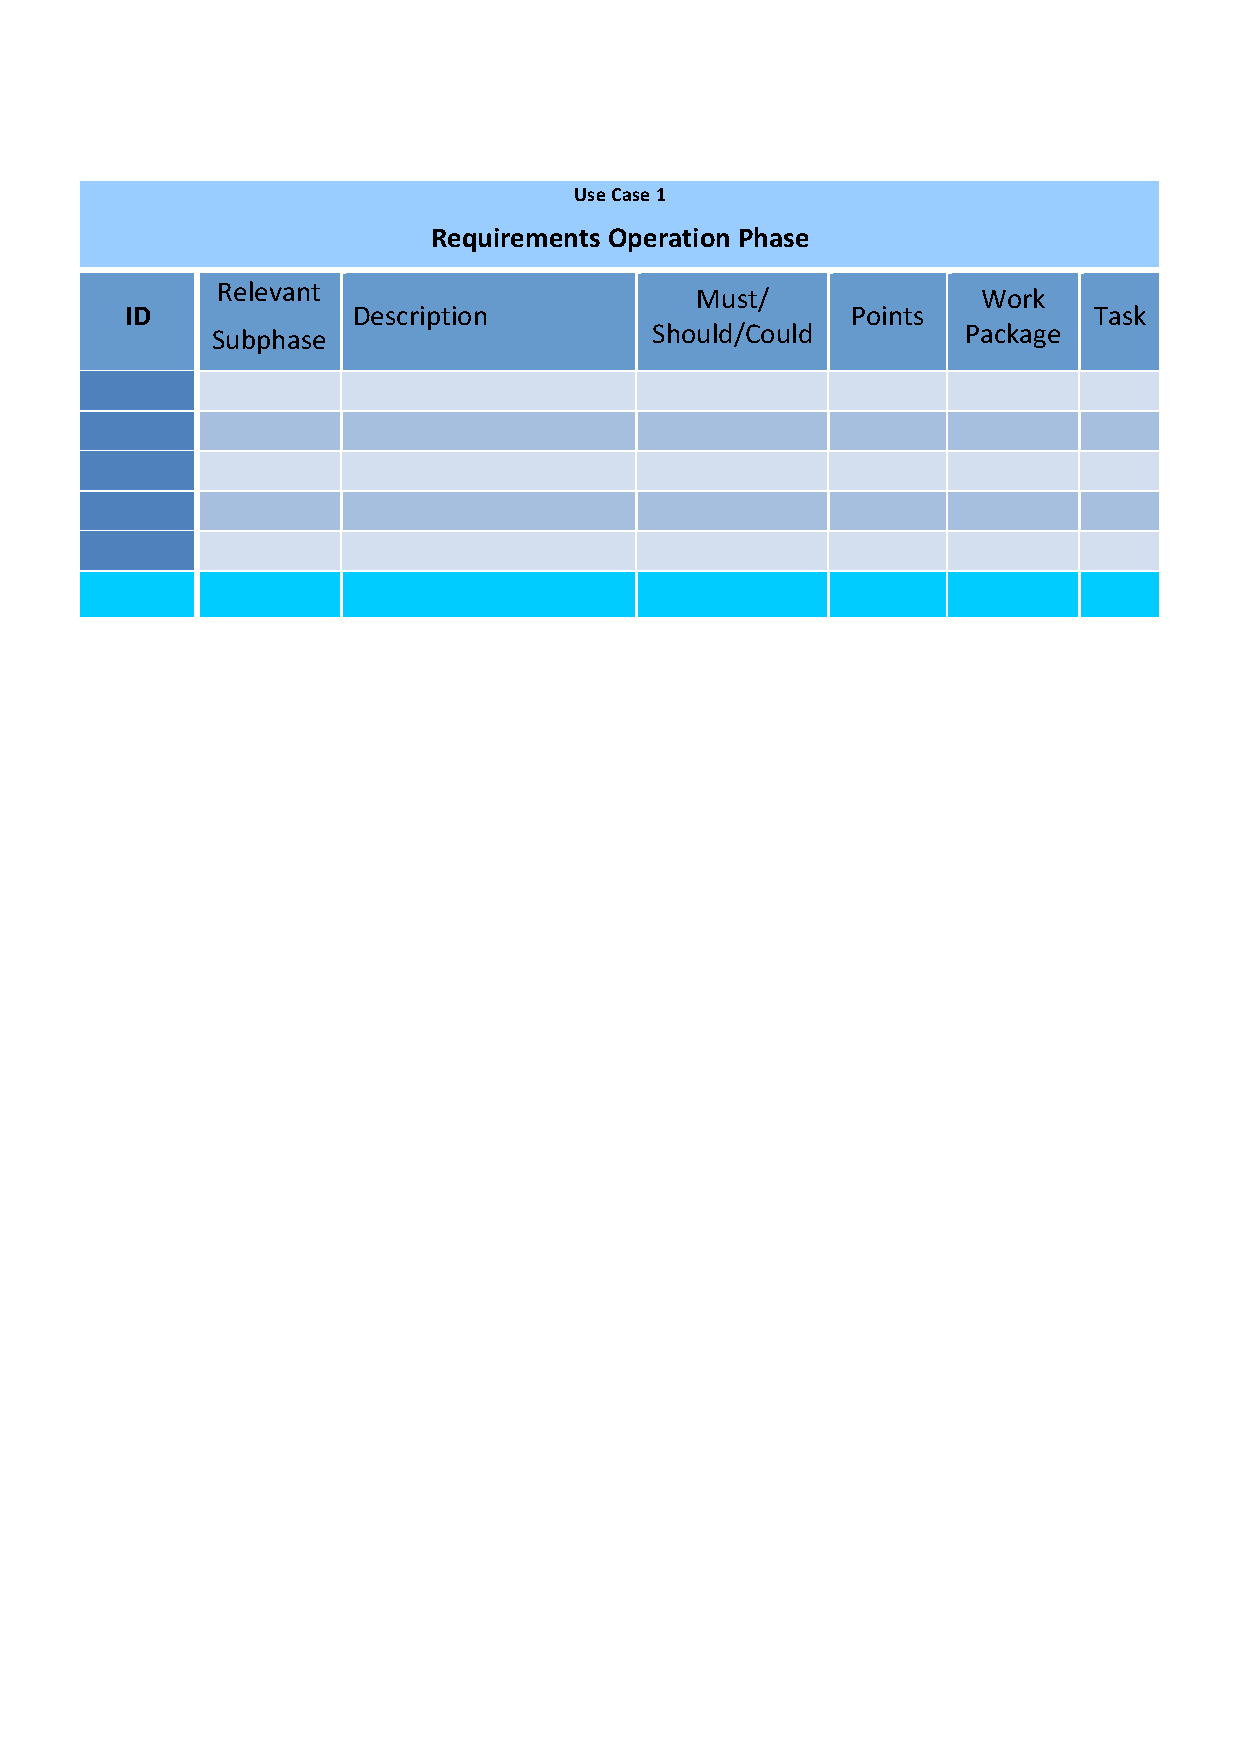
\includepdf[offset=0 1cm,scale=0.85,pages={-},pagecommand={\pagestyle{fancy}}]{appendixA2.pdf}
%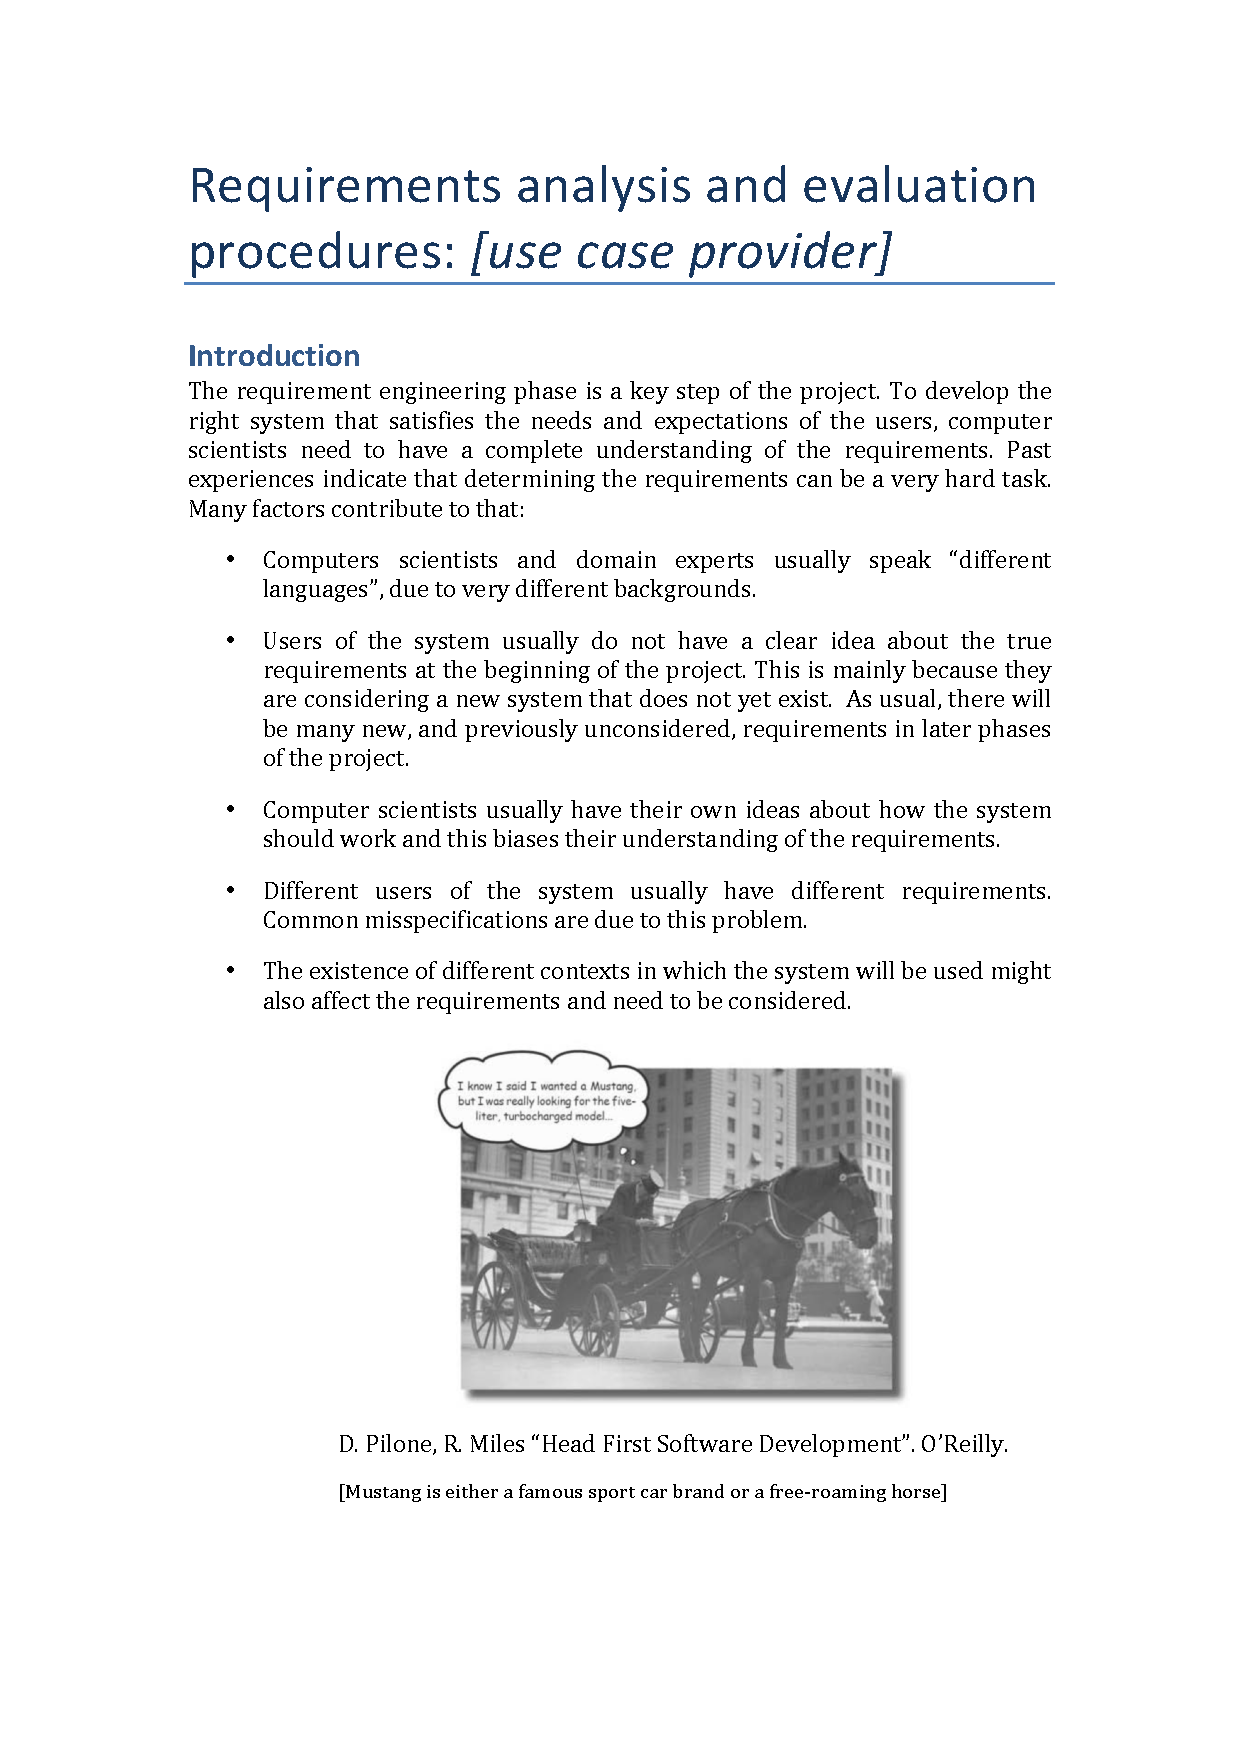
\includepdf[offset=0 1cm,scale=0.85,pages={-},pagecommand={\pagestyle{fancy}}]{appendixA_reformat.pdf}


\end{document}  